\chapter{Galois 理论}

\section{基本定义}

在前一章中，我们证明了域 $F$ 的一个有限扩张的存在性，这个扩张含有给定多项式 $f(x)$ 的所有根，其中 $f(x)$ 的系数属于 $F$。Galois 理论（以 Évariste Galois，1811--1832 命名）的主要思想，是考察 $f(x)$ 的根的置换群同它的分裂域的代数结构之间的关系。这个联系由下一节的基本定理给出。它可以看作数学中一个重要思想的又一个（极其优美的）应用：一个（在我们这里是代数的）对象作用在另一个对象上，会给出关于二者的结构信息。

本节中我们引入所关心对象的术语和基本性质。令 $K$ 为一个域。

\noindent\textbf{定义.}
\begin{enumerate}[label=(\arabic*)]
\item $K$ 到它自身的一个同构称为 $K$ 的一个\emph{自同构}。$K$ 的自同构全体记为 $\operatorname{Aut}(K)$。若 $a\in K$，我们将把 $\sigma(a)$ 记作 $\sigma a$。
\item 自同构 $\sigma\in\operatorname{Aut}(K)$ 称为\emph{固定}元素 $a\in K$，如果 $\sigma a=a$。如果 $F$ 是 $K$ 的一个子集（例如一个子域），则称自同构 $\sigma$ \emph{固定} $F$，如果它固定 $F$ 的所有元素，即对所有 $a\in F$ 都有 $\sigma a=a$。
\end{enumerate}

注意，任何域至少有一个自同构，即恒等映射，记为 $1$，有时称为平凡自同构。域 $K$ 的素域由 $1\in K$ 生成，并且由于任意自同构 $\sigma$ 都把 $1$ 送到 $1$（也把 $0$ 送到 $0$），即 $\sigma(1)=1$，所以对素域中的所有 $a$ 都有 $\sigma a=a$。因此，域 $K$ 的任意自同构都固定它的素子域。特别地，我们看到 $\mathbb Q$ 和 $\mathbb F_p$ 只有平凡自同构：
\[
\operatorname{Aut}(\mathbb Q)=\{1\},\qquad \operatorname{Aut}(\mathbb F_p)=\{1\}.
\]

\noindent\textbf{定义.} 设 $K/F$ 是域扩张。记 $\operatorname{Aut}(K/F)$ 为 $K$ 的所有固定 $F$ 的自同构的集合。

注意，如果 $F$ 是 $K$ 的素子域，则 $\operatorname{Aut}(K)=\operatorname{Aut}(K/F)$，因为 $K$ 的每个自同构都自动固定 $F$。

如果 $\sigma$ 和 $\tau$ 是 $K$ 的自同构，则复合 $\sigma\tau$（以及复合 $\tau\sigma$，它未必相同）是有定义的，并且仍然是 $K$ 的自同构。

\noindent\textbf{命题 1.} $\operatorname{Aut}(K)$ 在复合下是一个群，并且 $\operatorname{Aut}(K/F)$ 是一个子群。

\begin{proof}
显然 $\operatorname{Aut}(K)$ 是一个群。如果 $\sigma$ 和 $\tau$ 是固定 $F$ 的 $K$ 的自同构，则 $\sigma\tau$ 和 $\sigma^{-1}$ 在 $F$ 上也都是恒等映射，这说明 $\operatorname{Aut}(K/F)$ 是子群。
\end{proof}

下面的命题对于确定代数扩张的自同构极为有用。

\noindent\textbf{命题 2.} 设 $K/F$ 是一个域扩张，并设 $\alpha\in K$ 在 $F$ 上代数。则对任意 $\sigma\in\operatorname{Aut}(K/F)$，$\sigma\alpha$ 是 $\alpha$ 在 $F$ 上的极小多项式的一个根；也就是说，$\operatorname{Aut}(K/F)$ 置换不可约多项式的根。等价地，任何系数在 $F$ 中且以 $\alpha$ 为根的多项式，也以 $\sigma\alpha$ 为根。

\begin{proof}
设 $\alpha$ 满足方程
\[
\alpha^n+a_{n-1}\alpha^{n-1}+\cdots+a_1\alpha+a_0=0,
\]
其中 $a_0,a_1,\ldots,a_{n-1}$ 是 $F$ 的元素。施以自同构 $\sigma$，得到（利用 $\sigma$ 是加法同态）
\[
\sigma(\alpha^n)+\sigma(a_{n-1}\alpha^{n-1})+\cdots+\sigma(a_1\alpha)+\sigma(a_0)=\sigma(0)=0.
\]
再利用 $\sigma$ 也是乘法同态，这变为
\[
(\sigma(\alpha))^n+\sigma(a_{n-1})(\sigma(\alpha))^{n-1}+\cdots+
\sigma(a_1)\sigma(\alpha)+\sigma(a_0)=0.
\]
由假设，$\sigma$ 固定 $F$ 的所有元素，所以 $\sigma(a_i)=a_i$，$i=0,1,\ldots,n-1$。因此
\[
(\sigma\alpha)^n+a_{n-1}(\sigma\alpha)^{n-1}+\cdots+a_1(\sigma\alpha)+a_0=0.
\]
这正是说 $\sigma\alpha$ 是 $F$ 上同一个多项式的根。命题得证。
\end{proof}

\paragraph{例}
\begin{enumerate}[label=(\arabic*)]
\item 令 $K=\mathbb Q(\sqrt2)$。如果 $\tau\in\operatorname{Aut}(\mathbb Q(\sqrt2))=\operatorname{Aut}(\mathbb Q(\sqrt2)/\mathbb Q)$，则 $\tau(\sqrt2)=\pm\sqrt2$，因为这是 $\sqrt2$ 的极小多项式的两个根。由于 $\tau$ 固定 $\mathbb Q$，这完全确定了 $\tau$：
\[
\tau(a+b\sqrt2)=a\pm b\sqrt2.
\]
映射 $\sqrt2\mapsto\sqrt2$ 只是 $\mathbb Q(\sqrt2)$ 的恒等自同构 $1$。映射
\[
\sigma:\sqrt2\mapsto-\sqrt2
\]
是推论 13.7 后的例 2 中考虑的同构。因此
\[
\operatorname{Aut}(\mathbb Q(\sqrt2))=\operatorname{Aut}(\mathbb Q(\sqrt2)/\mathbb Q)=\{1,\sigma\}
\]
是由 $\sigma$ 生成的 $2$ 阶循环群。

\item 令 $K=\mathbb Q(\sqrt[3]{2})$。如前所述，如果 $\tau\in\operatorname{Aut}(K/\mathbb Q)$，则 $\tau$ 完全由它在 $\sqrt[3]{2}$ 上的作用确定，因为
\[
\tau(a+b\sqrt[3]{2}+c(\sqrt[3]{2})^2)=a+b\tau\sqrt[3]{2}+c(\tau\sqrt[3]{2})^2.
\]
由于 $\tau\sqrt[3]{2}$ 必须是 $x^3-2$ 的根，而此方程的另外两个根不属于 $K$（回忆这个多项式的分裂域在 $\mathbb Q$ 上次数为 $6$），唯一可能是 $\tau\sqrt[3]{2}=\sqrt[3]{2}$，即 $\tau=1$。因此
\[
\operatorname{Aut}(\mathbb Q(\sqrt[3]{2})/\mathbb Q)=1
\]
是平凡群。
\end{enumerate}

一般地，如果 $K$ 在 $F$ 上由某个元素集合生成，那么 $\operatorname{Aut}(K/F)$ 中的任意自同构 $\sigma$ 完全由它在这些生成元上的作用决定。如果 $K/F$ 有限，那么 $K$ 在 $F$ 上由有限多个代数元素生成，所以由命题可知，固定 $F$ 的 $K$ 的自同构数目有限，即 $\operatorname{Aut}(K/F)$ 是有限群。特别地，有限扩张的自同构可以看作有限多个方程的根的置换（然而并非每个置换都给出自同构，如上面的例 2 所说明）。正是对方程根的置换的研究，把 Galois 引向了我们正在描述的理论。

我们已经把一个群 $\operatorname{Aut}(K/F)$，即固定 $F$ 的 $K$ 的自同构群，与每个域扩张 $K/F$（等价地，与 $K$ 的子域 $F$）联系起来。也可以反过来，从一个自同构群联系到一个域扩张。

\noindent\textbf{命题 3.} 设 $H\leq \operatorname{Aut}(K)$ 是 $K$ 的自同构群的一个子群。那么 $K$ 中被 $H$ 的所有元素固定的元素集合 $F$ 是 $K$ 的一个子域。

\begin{proof}
令 $h\in H$，并令 $a,b\in F$。于是由定义 $h(a)=a$、$h(b)=b$，所以
\[
h(a\pm b)=h(a)\pm h(b)=a\pm b,
\]
\[
h(ab)=h(a)h(b)=ab,
\]
并且
\[
h(a^{-1})=h(a)^{-1}=a^{-1}.
\]
因此 $F$ 封闭，故为 $K$ 的子域。
\end{proof}

注意，在这个命题中，$H$ 实际上是 $\operatorname{Aut}(K)$ 的一个子群并不重要——$K$ 中被 $\operatorname{Aut}(K)$ 的一个子集的所有元素固定的元素集合也仍是 $K$ 的一个子域。

\noindent\textbf{定义.} 如果 $H$ 是 $K$ 的自同构群的一个子群，则 $K$ 中被 $H$ 的所有元素固定的子域称为 $H$ 的\emph{固定域}。

\noindent\textbf{命题 4.} 上面定义的由域到群、由群到域的对应是反包含的，即
\begin{enumerate}[label=(\arabic*)]
\item 如果 $F_1\subseteq F_2\subseteq K$ 是 $K$ 的两个子域，则
\[
\operatorname{Aut}(K/F_2)\leq \operatorname{Aut}(K/F_1),
\]
并且
\item 如果 $H_1\leq H_2\leq \operatorname{Aut}(K)$ 是两个自同构子群，其相应固定域分别为 $F_1$ 和 $F_2$，则 $F_2\subseteq F_1$。
\end{enumerate}

\begin{proof}
固定 $F_2$ 的任意 $K$ 的自同构也固定它的子域 $F_1$，这给出 (1)。第二个断言类似证明。
\end{proof}

\paragraph{例}
\begin{enumerate}[label=(\arabic*)]
\item 设 $K=\mathbb Q(\sqrt2)$，如上例 1。则 $\operatorname{Aut}(\mathbb Q(\sqrt2))=\operatorname{Aut}(\mathbb Q(\sqrt2)/\mathbb Q)=\{1,\sigma\}$ 的固定域是 $\mathbb Q(\sqrt2)$ 中满足
\[
\sigma(a+b\sqrt2)=a+b\sqrt2
\]
的元素集合，因为每个元素都被恒等自同构固定。这就是方程
\[
a-b\sqrt2=a+b\sqrt2,
\]
它等价于 $b=0$，所以 $\operatorname{Aut}(\mathbb Q(\sqrt2)/\mathbb Q)$ 的固定域就是 $\mathbb Q$。

\item 现在设 $K=\mathbb Q(\sqrt[3]{2})$，如上例 2。在此情形中 $\operatorname{Aut}(K)=1$，所以 $K$ 的每个元素都被固定，即 $\operatorname{Aut}(\mathbb Q(\sqrt[3]{2})/\mathbb Q)$ 的固定域是 $\mathbb Q(\sqrt[3]{2})$。
\end{enumerate}

给定 $K$ 的一个子域 $F$，对应的群是固定 $F$ 的 $K$ 的自同构集合。给定 $K$ 的一个自同构群，则通过取这些自同构的固定域来定义相应的扩张。在上面的第一个例子中，从 $\mathbb Q(\sqrt2)$ 的子域 $\mathbb Q$ 出发，得到群 $\{1,\sigma\}$；再从群 $\{1,\sigma\}$ 出发，又得到子域 $\mathbb Q$，所以二者之间存在一种“对偶”。然而在第二个例子中，从 $\mathbb Q(\sqrt[3]{2})$ 的子域 $\mathbb Q$ 出发，只得到平凡群；再从平凡群出发，得到整个域 $\mathbb Q(\sqrt[3]{2})$。

考察这两个例子提示我们：在第二个例子中，自同构“不够多”，不能迫使固定域为 $\mathbb Q$，而只能得到整个 $\mathbb Q(\sqrt[3]{2})$。这又似乎是因为 $x^3-2$ 的其他根，也就是自同构下 $\sqrt[3]{2}$ 的唯一可能像，并不是 $\mathbb Q(\sqrt[3]{2})$ 的元素。（不过即使它们属于该域，我们也还需要检查由此定义的附加映射是否真的是自同构。）现在我们精确地定义带有“足够多”自同构的域（这将导向 Galois 扩张的定义）。正如甚至从这两个例子就可能猜到的那样（我们将在下一节证明），这些域与分裂域有关。

我们首先考察分裂域情形中自同构群的大小。设 $F$ 是一个域，并设 $E$ 是 $F$ 上 $f(x)\in F[x]$ 的分裂域。主要工具是关于同构延拓存在性的定理 13.27，它断言：$F$ 与 $F'$ 的任意同构 $\varphi:F\xrightarrow{\sim}F'$ 都能延拓为同构 $\sigma:E\xrightarrow{\sim}E'$，其中 $E'$ 是 $f'(x)=\varphi(f(x))\in F'[x]$ 的分裂域。

我们现在用对 $[E:F]$ 的归纳证明，这样的延拓数目至多为 $[E:F]$，并且如果 $f(x)$ 在 $F$ 上可分，则等号成立。如果 $[E:F]=1$，则 $E=F$、$E'=F'$、$\sigma=\varphi$，延拓的数目为 $1$。如果 $[E:F]>1$，那么 $f(x)$ 至少有一个次数 $>1$ 的不可约因子 $p(x)$，并有 $f'(x)$ 的相应不可约因子 $p'(x)$。令 $\alpha$ 为 $p(x)$ 的一个固定根。如果 $\sigma$ 是 $\varphi$ 到 $E$ 的任意延拓，那么 $\sigma$ 限制在 $E$ 的子域 $F(\alpha)$ 上，是 $F(\alpha)$ 到 $E'$ 的某个子域的同构 $\tau$。同构 $\tau$ 完全由它在 $\alpha$ 上的作用，即由 $\tau\alpha$，决定，因为 $\alpha$ 在 $F$ 上生成 $F(\alpha)$。正如在命题 2 中一样，我们看到 $\tau\alpha$ 必须是 $p'(x)$ 的某个根 $\beta$。于是有图
\[
\begin{array}{ccccc}
\sigma:& E & \longrightarrow & E'& \\
& | && |& \\
\tau:& F(\alpha)& \longrightarrow & F'(\beta)& \\
& | && |& \\
\varphi:& F & \longrightarrow & F'& .
\end{array}
\]
反过来，对 $p'(x)$ 的任意根 $\beta$，都存在给出这种图的延拓 $\tau$ 和 $\sigma$（这就是定理 13.8 和定理 13.27）。因此，为了计算延拓 $\sigma$ 的数目，只需要计算这种图的可能数目。

$\varphi$ 到同构 $\tau$ 的延拓数等于 $p'(x)$ 的不同根的数目。由于 $p(x)$ 和 $p'(x)$ 的次数都等于 $[F(\alpha):F]$，我们看到 $\varphi$ 到 $\tau$ 的延拓数至多为 $[F(\alpha):F]$；如果 $p(x)$ 的根互异，则等号成立。

由于 $E$ 也是 $f(x)$ 在 $F(\alpha)$ 上的分裂域，$E'$ 是 $f'(x)$ 在 $F'(\beta)$ 上的分裂域，并且 $[E:F(\alpha)]<[E:F]$，我们可以把归纳假设应用于这些域扩张。由归纳可知，$\tau$ 到 $\sigma$ 的延拓数至多为 $[E:F(\alpha)]$；如果 $f(x)$ 的根互异，则等号成立。

由
\[
[E:F]=[E:F(\alpha)][F(\alpha):F]
\]
可知，$\varphi$ 到 $\sigma$ 的延拓数至多为 $[E:F]$。如果 $p(x)$ 和 $f(x)$ 都有互异根，则等号成立；这等价于 $f(x)$ 有互异根，因为 $p(x)$ 是 $f(x)$ 的因子。归纳证明完成。

在特殊情形 $F=F'$ 且 $\varphi$ 是恒等映射时，有 $f(x)=f'(x)$ 且 $E=E'$，于是 $E$ 到 $E'$ 的、限制到 $F$ 上为 $\varphi$ 的同构，正是固定 $F$ 的 $E$ 的自同构。我们把这表述如下：

\noindent\textbf{命题 5.} 设 $E$ 是多项式 $f(x)\in F[x]$ 在 $F$ 上的分裂域。则
\[
|\operatorname{Aut}(E/F)|\leq [E:F],
\]
如果 $f(x)$ 在 $F$ 上可分，则等号成立。

\paragraph{注记：} 虽然我们主要关心的是计算固定 $F$ 的 $E$ 的自同构（即上面 $F=F'$、$\varphi=1$ 的情形），但是仍然必须考虑更一般的 $\varphi$（以及不同的域 $F'$），因为证明中的归纳步骤涉及同一个多项式 $p(x)$ 的两个根对应的域 $F(\alpha)$ 与 $F(\beta)$。

可以修改上面的证明，更一般地证明对任意有限扩张 $K/F$ 都有 $|\operatorname{Aut}(K/F)|\leq [K:F]$（我们将在下一节从稍微不同的观点证明这一点）。这给出具有“足够多”自同构的域扩张的概念。

\noindent\textbf{定义.} 设 $K/F$ 是有限扩张。如果 $|\operatorname{Aut}(K/F)|=[K:F]$，则称 $K$ 在 $F$ 上是 \emph{Galois} 的，并称 $K/F$ 是一个 \emph{Galois 扩张}。如果 $K/F$ 是 Galois 的，则自同构群 $\operatorname{Aut}(K/F)$ 称为 $K/F$ 的 \emph{Galois 群}，记为 $\operatorname{Gal}(K/F)$。

\paragraph{注记：} 对任意 $K/F$，扩张 $K/F$ 的 Galois 群有时被定义为自同构群 $\operatorname{Aut}(K/F)$。我们采用上面的定义，是为了使记号 $\operatorname{Gal}(K/F)$ 强调扩张 $K/F$ 有最大可能数目的自同构。

\noindent\textbf{推论 6.} 如果 $K$ 是可分多项式 $f(x)$ 在 $F$ 上的分裂域，则 $K/F$ 是 Galois 的。

我们将在下一节看到其逆命题也为真，这将完全刻画 Galois 扩张。

还要注意，推论 6 蕴含任意多项式在 $\mathbb Q$ 上的分裂域都是 Galois 的，因为 $f(x)$ 的分裂域显然与 $f(x)$ 的不可约因子的乘积（即去掉重因子后得到的多项式）的分裂域相同，而后者是可分的（推论 13.34）。

\noindent\textbf{定义.} 如果 $f(x)$ 是 $F$ 上的可分多项式，则 $f(x)$ 在 $F$ 上的 \emph{Galois 群}是 $f(x)$ 的分裂域在 $F$ 上的 Galois 群。

\paragraph{例}
\begin{enumerate}[label=(\arabic*)]
\item 扩张 $\mathbb Q(\sqrt2)/\mathbb Q$ 是 Galois 的，其 Galois 群为
\[
\operatorname{Gal}(\mathbb Q(\sqrt2)/\mathbb Q)=\{1,\sigma\}\cong \mathbb Z/2\mathbb Z,
\]
其中 $\sigma$ 是自同构
\[
\sigma: \mathbb Q(\sqrt2)\longrightarrow \mathbb Q(\sqrt2),\qquad
 a+b\sqrt2\longmapsto a-b\sqrt2.
\]

\item 更一般地，任意特征不为 $2$ 的域 $F$ 的二次扩张 $K$ 都是 Galois 的。这来自推论 13.13 后关于二次扩张的讨论，该讨论说明 $F$ 的任意 $2$ 次扩张 $K$（当 $F$ 的特征不为 $2$ 时）具有形式 $F(\sqrt D)$，因而是 $x^2-D$ 的分裂域（因为若 $\sqrt D\in K$，则 $-\sqrt D\in K$）。

\item 扩张 $\mathbb Q(\sqrt[3]{2})/\mathbb Q$ 不是 Galois 的，因为它的自同构群只有 $1$ 个元素。

\item 扩张 $\mathbb Q(\sqrt2,\sqrt3)$ 在 $\mathbb Q$ 上是 Galois 的，因为它是多项式 $(x^2-2)(x^2-3)$ 的分裂域。任意自同构 $\sigma$ 完全由它在生成元 $\sqrt2$ 和 $\sqrt3$ 上的作用决定，而这两个元素必须分别被送到 $\pm\sqrt2$ 和 $\pm\sqrt3$。因此自同构唯一可能为映射
\[
\begin{array}{c|c|c|c}
\sqrt2\mapsto\sqrt2 & \sqrt2\mapsto-\sqrt2 & \sqrt2\mapsto\sqrt2 & \sqrt2\mapsto-\sqrt2\\
\sqrt3\mapsto\sqrt3 & \sqrt3\mapsto\sqrt3 & \sqrt3\mapsto-\sqrt3 & \sqrt3\mapsto-\sqrt3
\end{array}
\]
由于 Galois 群阶为 $4$，所有这些元素事实上都是 $\mathbb Q(\sqrt2,\sqrt3)$ 在 $\mathbb Q$ 上的自同构。

定义自同构 $\sigma$ 和 $\tau$ 为
\[
\sigma:\left\{
\begin{array}{l}
\sqrt2\mapsto-\sqrt2,\\
\sqrt3\mapsto\sqrt3,
\end{array}\right.
\qquad
\tau:\left\{
\begin{array}{l}
\sqrt2\mapsto\sqrt2,\\
\sqrt3\mapsto-\sqrt3,
\end{array}\right.
\]
或者更明确地，定义为
\[
\sigma: a+b\sqrt2+c\sqrt3+d\sqrt6\longmapsto a-b\sqrt2+c\sqrt3-d\sqrt6
\]
和
\[
\tau: a+b\sqrt2+c\sqrt3+d\sqrt6\longmapsto a+b\sqrt2-c\sqrt3-d\sqrt6
\]
（因为例如
\[
\sigma(\sqrt6)=\sigma(\sqrt2\sqrt3)=\sigma(\sqrt2)\sigma(\sqrt3)=(-\sqrt2)(\sqrt3)=-\sqrt6
\]
）。
于是 $\sigma^2(\sqrt2)=\sigma(\sigma\sqrt2)=\sigma(-\sqrt2)=\sqrt2$，并且显然 $\sigma^2(\sqrt3)=\sqrt3$。因此 $\sigma^2=1$ 是恒等自同构。类似地，$\tau^2=1$。自同构 $\sigma\tau$ 可直接计算：
\[
\sigma\tau(\sqrt2)=\sigma(\tau(\sqrt2))=\sigma(\sqrt2)=-\sqrt2
\]
且
\[
\sigma\tau(\sqrt3)=\sigma(\tau(\sqrt3))=\sigma(-\sqrt3)=-\sqrt3.
\]
因此 $\sigma\tau$ 是 Galois 群中剩下的非平凡自同构。由于这个自同构显然在 Galois 群中也有阶 $2$，我们有
\[
\operatorname{Gal}(\mathbb Q(\sqrt2,\sqrt3)/\mathbb Q)=\{1,\sigma,\tau,\sigma\tau\},
\]
即 Galois 群同构于 Klein 四元群。

与 $\operatorname{Gal}(\mathbb Q(\sqrt2,\sqrt3)/\mathbb Q)$ 的每个子群相联系的是 $\mathbb Q(\sqrt2,\sqrt3)$ 的相应固定子域。例如，与 $\{1,\sigma\tau\}$ 相应的子域是被映射
\[
\sigma\tau:a+b\sqrt2+c\sqrt3+d\sqrt6\longmapsto a-b\sqrt2-c\sqrt3+d\sqrt6
\]
固定的元素集合，这就是元素 $a+d\sqrt6$ 的集合，即域 $\mathbb Q(\sqrt6)$。类似地可以确定 Galois 群的其他子群的固定域：
\[
\begin{array}{c|c}
\text{子群} & \text{固定域}\\ \hline
\{1\} & \mathbb Q(\sqrt2,\sqrt3)\\
\{1,\sigma\} & \mathbb Q(\sqrt3)\\
\{1,\sigma\tau\} & \mathbb Q(\sqrt6)\\
\{1,\tau\} & \mathbb Q(\sqrt2)\\
\{1,\sigma,\tau,\sigma\tau\} & \mathbb Q
\end{array}
\]

\item $x^3-2$ 在 $\mathbb Q$ 上的分裂域是 $6$ 次 Galois 扩张。这个方程的根为
\[
\sqrt[3]{2},\quad \rho\sqrt[3]{2},\quad \rho^2\sqrt[3]{2},
\]
其中
\[
\rho=\frac{-1+\sqrt{-3}}{2}
\]
是一个本原三次单位根。因此分裂域可写为 $\mathbb Q(\sqrt[3]{2},\rho\sqrt[3]{2})$。任意自同构把这两个元素各自送到 $x^3-2$ 的某个根，给出 $9$ 种可能；但由于 Galois 群阶为 $6$，并非每个这样的映射都是域的自同构。

为了确定 Galois 群，我们使用一组更方便的生成元，即 $\sqrt[3]{2}$ 和 $\rho$。任意自同构 $\sigma$ 把 $\sqrt[3]{2}$ 送到 $\sqrt[3]{2}$、$\rho\sqrt[3]{2}$、$\rho^2\sqrt[3]{2}$ 之一，并把 $\rho$ 送到
\[
\rho\quad\text{或}\quad \rho^2=\frac{-1-\sqrt{-3}}{2},
\]
因为它们是分圆多项式 $\Phi_3(x)=x^2+x+1$ 的根。由于 $\sigma$ 完全由它在这两个元素上的作用决定，这只给出 $6$ 种可能，因而每一种可能事实上都是自同构。为了明确给出这些自同构，令 $\sigma$ 和 $\tau$ 为
\[
\sigma:\left\{
\begin{array}{l}
\sqrt[3]{2}\mapsto \rho\sqrt[3]{2},\\
\rho\mapsto \rho,
\end{array}\right.
\qquad
\tau:\left\{
\begin{array}{l}
\sqrt[3]{2}\mapsto \sqrt[3]{2},\\
\rho\mapsto \rho^2=-1-\rho.
\end{array}\right.
\]
与前面一样，这些映射可以在 $\mathbb Q(\sqrt[3]{2},\rho)$ 的元素上明确给出，而这些元素是基
\[
\{1,\sqrt[3]{2},(\sqrt[3]{2})^2,\rho,\rho\sqrt[3]{2},\rho(\sqrt[3]{2})^2\}
\]
的线性组合。例如
\[
\sigma(\rho\sqrt[3]{2})=(\rho)(\rho\sqrt[3]{2})=\rho^2\sqrt[3]{2}=(-1-\rho)\sqrt[3]{2}
=-\sqrt[3]{2}-\rho\sqrt[3]{2},
\]
并且可以类似地确定 $\sigma$ 在其他基元素上的作用。这给出
\[
\begin{aligned}
\sigma:&\ a+b\sqrt[3]{2}+c\sqrt[3]{4}+d\rho+e\rho\sqrt[3]{2}+f\rho\sqrt[3]{4} \\
&\longmapsto
 a-e\sqrt[3]{2}+(f-c)\sqrt[3]{4}+d\rho+(b-e)\rho\sqrt[3]{2}-c\rho\sqrt[3]{4}.
\end{aligned}
\tag{14.1}
\]
Galois 群的其他元素是
\[
1:\left\{
\begin{array}{l}
\sqrt[3]{2}\mapsto\sqrt[3]{2},\\
\rho\mapsto\rho,
\end{array}\right.
\qquad
\sigma^2:\left\{
\begin{array}{l}
\sqrt[3]{2}\mapsto\rho^2\sqrt[3]{2},\\
\rho\mapsto\rho,
\end{array}\right.
\]
计算 $\sigma\tau$ 得到
\[
\sigma\tau:\left\{
\begin{array}{l}
\sqrt[3]{2}\mapsto \sqrt[3]{2}\mapsto \rho\sqrt[3]{2},\\
\rho\mapsto \rho^2\mapsto \rho^2,
\end{array}\right.
\]
即
\[
\sigma\tau:\left\{
\begin{array}{l}
\sqrt[3]{2}\mapsto \rho\sqrt[3]{2},\\
\rho\mapsto \rho^2.
\end{array}\right.
\]
所以 $\sigma\tau=\tau\sigma^2$。类似地可算得 $\sigma^3=\tau^2=1$。因此
\[
\operatorname{Gal}(\mathbb Q(\sqrt[3]{2},\rho)/\mathbb Q)=\langle \sigma,\tau
angle\cong S_3
\]
是 $3$ 个字母上的对称群。或者（并且计算更少地）说，由于
\[
G=\operatorname{Gal}(\mathbb Q(\sqrt[3]{2},\rho)/\mathbb Q)
\]
作为 $x^3-2$ 的 $3$ 个根的置换来作用，$G$ 是 $S_3$ 的一个子群，所以既然它的阶为 $6$，就必须是 $S_3$。上面的计算明确地识别了 $G$ 中的自同构，并给出 $G$ 与 $S_3$ 的一个显式同构。

和前面的例子一样，我们可以确定 Galois 群任意子群的固定域。例如，考虑由 $\sigma$ 生成的子群 $\{1,\sigma,\sigma^2\}$ 的固定域。它们正是被 $\sigma$ 固定的元素（见等式 (14.1) 中的显式公式），因为如果一个元素被 $\sigma$ 固定，那么也被 $\sigma^2$ 固定。（一般地，某个子群的固定域就是被该子群的一组生成元固定的域。）被 $\sigma$ 固定的元素是满足
\[
a=a,\\qquad b=-e,
\qquad c=f-c,
\qquad d=d,
\qquad e=b-e,
\qquad f=-c
\]
的元素，这等价于 $b=c=f=e=0$。因此 $\{1,\sigma,\sigma^2\}$ 的固定域是 $\mathbb Q(\rho)$。

\paragraph{注记：} 这个例子说明，在由生成元的作用确定 Galois 群时必须谨慎。如上所述，并不是每个把 $\sqrt[3]{2}$ 和 $\rho\sqrt[3]{2}$ 送到 $x^3-2$ 的根的映射，都产生域的自同构（例如，映射
\[
\sqrt[3]{2}\mapsto \rho\sqrt[3]{2},\qquad
\rho\sqrt[3]{2}\mapsto \rho\sqrt[3]{2}
\]
显然不可能是自同构，因为它显然不是单射）。关键在于生成元之间可能存在（有时非常微妙的）代数关系，而这些关系必须被自同构保持。例如，这里的两个生成元之商是 $\rho$，它在上面的映射下被送到 $1$，而不是 $\rho$ 的极小多项式的根。换句话说，这些生成元之商满足一个二次方程，而该映射不保持这一性质。

另一个（不那么平凡的）例子，可与第 2 节中关于 $x^8-2$ 的分裂域的讨论比较。

\item 如例 3 中所述，域 $\mathbb Q(\sqrt[4]{2})$ 在 $\mathbb Q$ 上不是 Galois 的，因为任意自同构都由它把 $\sqrt[4]{2}$ 送到何处决定，而在四种可能 $\{\pm\sqrt[4]{2},\pm i\sqrt[4]{2}\}$ 中，只有两个是该域的元素（两个实根）。

注意我们有
\[
\begin{array}{ccccc}
\mathbb Q & \subset & \mathbb Q(\sqrt2) & \subset & \mathbb Q(\sqrt[4]{2})\\
& 2 && 2 &
\end{array}
\]
其中 $\mathbb Q(\sqrt2)/\mathbb Q$ 和 $\mathbb Q(\sqrt[4]{2})/\mathbb Q(\sqrt2)$ 都由例 2 是 Galois 扩张，因为二者都是二次扩张。这说明一个 Galois 扩张的 Galois 扩张未必是 Galois 的。

\item 推论 6 表明，命题 13.37 之后构造的有限域扩张 $\mathbb F_{p^n}/\mathbb F_p$ 是 Galois 的，因为 $\mathbb F_{p^n}$ 是可分多项式 $x^{p^n}-x$ 在 $\mathbb F_p$ 上的分裂域。由此可知，这个扩张的自同构群阶为 $n$。命题 13.35 中的单射同态
\[
\sigma:\mathbb F_{p^n}\longrightarrow \mathbb F_{p^n},\qquad \alpha\longmapsto \alpha^p
\]
在此情形中是满射，因为 $\mathbb F_{p^n}$ 是有限的，所以它是同构。这给出 $\mathbb F_{p^n}$ 的一个自同构，称为 \emph{Frobenius 自同构}，我们记为 $\sigma_p$。迭代 $\sigma_p$，有
\[
\sigma_p^2(\alpha)=\sigma_p(\sigma_p(\alpha))=(\alpha^p)^p=\alpha^{p^2}.
\]
类似地，
\[
\sigma_p^i(\alpha)=\alpha^{p^i},\qquad i=0,1,2,\ldots
\]
由于 $\alpha^{p^n}=\alpha$，我们看到 $\sigma_p^n=1$ 是恒等自同构。$\sigma_p$ 的更低正幂不可能为恒等，因为这将意味着对某个 $i<n$，所有 $\alpha\in\mathbb F_{p^n}$ 都满足 $\alpha^{p^i}=\alpha$，这是不可能的，因为这个方程只有 $p^i$ 个根。由此可知 $\sigma_p$ 在 Galois 群中阶为 $n$，也就是说 $\operatorname{Gal}(\mathbb F_{p^n}/\mathbb F_p)$ 是 $n$ 阶循环群，以 Frobenius 自同构 $\sigma_p$ 为生成元。

\item 第 13.5 节中考虑的不可分扩张 $\mathbb F_2(x)$ 在 $\mathbb F_2(t)$ 上（其中 $x^2-t=0$）不是 Galois 的。这个二次扩张的任意自同构由它在 $x$ 上的作用决定，而 $x$ 必须被送到方程 $X^2-t$ 的一个根。我们已经看到这个方程只有一个根（重数为 $2$），因为我们在特征 $2$ 的域中。因此这个扩张只有平凡自同构。注意，$\mathbb F_2(x)$ 是 $X^2-t$ 在 $\mathbb F_2(t)$ 上的分裂域，所以这个例子说明推论 6 中的可分性条件是必要的。
\end{enumerate}

\subsection*{练习}

\begin{enumerate}[label=\arabic*.]
\item
\begin{enumerate}[label=(\alph*)]
\item 证明：如果域 $K$ 在 $F$ 上由元素 $\alpha_1,\ldots,\alpha_n$ 生成，那么固定 $F$ 的 $K$ 的自同构 $\sigma$ 由 $\sigma(\alpha_1),\ldots,\sigma(\alpha_n)$ 唯一决定。特别地，证明一个自同构固定 $K$ 当且仅当它固定 $K$ 的一组生成元。
\item 设 $G\leq \operatorname{Gal}(K/F)$ 是扩张 $K/F$ 的 Galois 群的一个子群，并设 $\sigma_1,\ldots,\sigma_k$ 是 $G$ 的生成元。证明子域 $E/F$ 被 $G$ 固定当且仅当它被生成元 $\sigma_1,\ldots,\sigma_k$ 固定。
\end{enumerate}

\item 令 $\tau$ 为映射 $\tau:\mathbb C\to\mathbb C$，定义为 $\tau(a+bi)=a-bi$（复共轭）。证明 $\tau$ 是 $\mathbb C$ 的自同构。

\item 求复共轭在 $\mathbb C$ 上的固定域。

\item 证明 $\mathbb Q(\sqrt2)$ 与 $\mathbb Q(\sqrt3)$ 不同构。

\item 明确确定扩张 $\mathbb Q(\sqrt[4]{2})/\mathbb Q(\sqrt2)$ 的自同构。

\item 设 $k$ 是域。
\begin{enumerate}[label=(\alph*)]
\item 证明：对固定的 $a,b\in k$、$a\neq0$，由
\[
\varphi(f(t))=f(at+b)
\]
定义的映射 $\varphi:k[t]\to k[t]$ 是 $k[t]$ 的一个自同构，并且在 $k$ 上为恒等。
\item 反过来，设 $\varphi$ 是 $k[t]$ 的一个自同构，并且在 $k$ 上为恒等。证明存在 $a,b\in k$ 且 $a\neq0$，使得 $\varphi(f(t))=f(at+b)$，如 (a) 中所述。
\end{enumerate}

\item 本练习确定 $\operatorname{Aut}(\mathbb R/\mathbb Q)$。
\begin{enumerate}[label=(\alph*)]
\item 证明任意 $\sigma\in\operatorname{Aut}(\mathbb R/\mathbb Q)$ 把平方送到平方，并把正实数送到正实数。推出对任意 $a,b\in\mathbb R$，若 $a<b$，则 $\sigma a<\sigma b$。
\item 证明若
\[
-\frac1m<a-b<\frac1m
\]
则
\[
-\frac1m<\sigma a-\sigma b<\frac1m
\]
对每个正整数 $m$ 成立。推出 $\sigma$ 是 $\mathbb R$ 上的连续映射。
\item 证明任何在 $\mathbb Q$ 上为恒等的 $\mathbb R$ 上连续映射都是恒等映射，因此 $\operatorname{Aut}(\mathbb R/\mathbb Q)=1$。
\end{enumerate}

\item 证明固定 $k$ 的有理函数域 $k(t)$ 的自同构，恰好是由
\[
t\longmapsto \frac{at+b}{ct+d}
\]
确定的分式线性变换，其中 $a,b,c,d\in k$ 且 $ad-bc\neq0$（于是 $f(t)\in k(t)$ 被送到
\[
f\left(\frac{at+b}{ct+d}\right)
\]
）（参见第 13.2 节练习 18）。

\item 求 $k(t)$ 的自同构 $t\mapsto t+1$ 的固定域。

\item 设 $K$ 是域 $F$ 的一个扩张。令 $\varphi:K\to K'$ 是 $K$ 与域 $K'$ 的一个同构，它把 $F$ 映到 $K'$ 的子域 $F'$。证明映射
\[
\sigma\longmapsto \varphi\sigma\varphi^{-1}
\]
定义一个群同构
\[
\operatorname{Aut}(K/F)\cong \operatorname{Aut}(K'/F').
\]
\end{enumerate}

\section{Galois 理论基本定理}

在上一节考虑的 Galois 扩张 $\operatorname{Gal}(\mathbb Q(\sqrt2,\sqrt3)/\mathbb Q)$ 中，Galois 群的子群图与相应固定域的图之间有很强的相似性：
\[
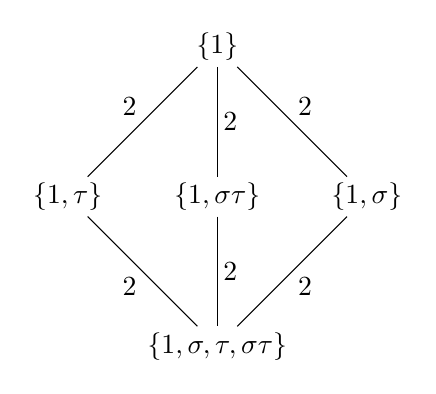
\begin{tikzpicture}[scale=0.95, baseline=(current bounding box.center), every node/.style={inner sep=2pt}]
\node (top) at (0,2) {$\{1\}$};
\node (l) at (-2,0) {$\{1,\tau\}$};
\node (m) at (0,0) {$\{1,\sigma\tau\}$};
\node (r) at (2,0) {$\{1,\sigma\}$};
\node (bot) at (0,-2) {$\{1,\sigma,\tau,\sigma\tau\}$};
\draw (top)-- node[above left] {$2$} (l);
\draw (top)-- node[right] {$2$} (m);
\draw (top)-- node[above right] {$2$} (r);
\draw (l)-- node[below left] {$2$} (bot);
\draw (m)-- node[right] {$2$} (bot);
\draw (r)-- node[below right] {$2$} (bot);
\end{tikzpicture}
\]
以及相应固定域的图
\[
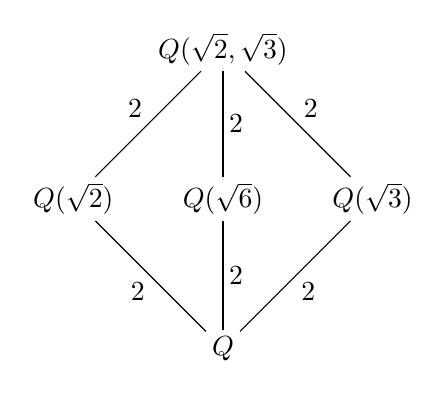
\begin{tikzpicture}[scale=0.95, baseline=(current bounding box.center), every node/.style={inner sep=2pt}]
\node (top) at (0,2) {$\mathbb Q(\sqrt2,\sqrt3)$};
\node (l) at (-2,0) {$\mathbb Q(\sqrt2)$};
\node (m) at (0,0) {$\mathbb Q(\sqrt6)$};
\node (r) at (2,0) {$\mathbb Q(\sqrt3)$};
\node (bot) at (0,-2) {$\mathbb Q$};
\draw (top)-- node[above left] {$2$} (l);
\draw (top)-- node[right] {$2$} (m);
\draw (top)-- node[above right] {$2$} (r);
\draw (l)-- node[below left] {$2$} (bot);
\draw (m)-- node[right] {$2$} (bot);
\draw (r)-- node[below right] {$2$} (bot);
\end{tikzpicture}
\]
（由于这种对应的反包含性质，我们已经把子群格倒置过来）。注意，这也是该扩张的所有已知子域的图，并且在这个情形中，每个子域本身也是 $\mathbb Q$ 上的 Galois 扩张。

类似地，Galois 群的子群图
\[
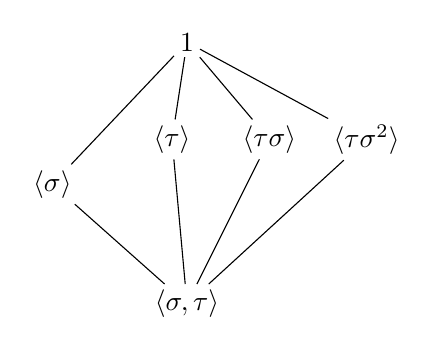
\begin{tikzpicture}[scale=0.95, baseline=(current bounding box.center), every node/.style={inner sep=2pt}]
\node (top) at (0,2.1) {$1$};
\node (a) at (-1.8,0.2) {$\langle\sigma\rangle$};
\node (t) at (-0.2,0.8) {$\langle\tau\rangle$};
\node (ta) at (1.1,0.8) {$\langle\tau\sigma\rangle$};
\node (ta2) at (2.4,0.8) {$\langle\tau\sigma^2\rangle$};
\node (bot) at (0,-1.4) {$\langle\sigma,\tau\rangle$};
\draw (top)--(a);
\draw (top)--(t);
\draw (top)--(ta);
\draw (top)--(ta2);
\draw (a)--(bot);
\draw (t)--(bot);
\draw (ta)--(bot);
\draw (ta2)--(bot);
\end{tikzpicture}
\]
与 $x^3-2$ 的分裂域的已知子域图也有很强的相似性：
\[
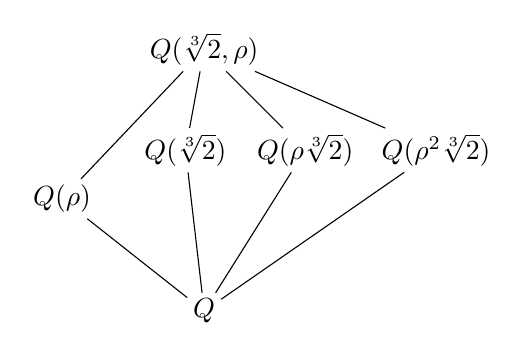
\begin{tikzpicture}[scale=0.95, baseline=(current bounding box.center), every node/.style={inner sep=2pt}]
\node (top) at (0,2.1) {$\mathbb Q(\sqrt[3]{2},\rho)$};
\node (rho) at (-1.9,0.1) {$\mathbb Q(\rho)$};
\node (a) at (-0.25,0.75) {$\mathbb Q(\sqrt[3]{2})$};
\node (b) at (1.35,0.75) {$\mathbb Q(\rho\sqrt[3]{2})$};
\node (c) at (3.1,0.75) {$\mathbb Q(\rho^2\sqrt[3]{2})$};
\node (bot) at (0,-1.4) {$\mathbb Q$};
\draw (top)--(rho);
\draw (top)--(a);
\draw (top)--(b);
\draw (top)--(c);
\draw (rho)--(bot);
\draw (a)--(bot);
\draw (b)--(bot);
\draw (c)--(bot);
\end{tikzpicture}
\]
第二个图中的子域正是第一个图中子群的固定域。注意，在这对图中，只有由 $\sigma$ 生成的子群 $\langle\sigma\rangle$ 是 $S_3$ 中的正规子群，而且子域 $\mathbb Q(\rho)$ 是唯一在 $\mathbb Q$ 上 Galois 的子域。

Galois 理论基本定理断言，在上面两个例子中观察到的关系不是偶然的，并且对任意 Galois 扩张都成立。在证明它之前，我们先发展一些关于群的特征的预备结果；域自同构将给出这种特征的特殊例子。

\noindent\textbf{定义.} 群 $G$ 的一个取值于域 $L$ 中的\emph{特征}\footnote{这是线性特征的定义。更一般的特征将在第 18 章中研究。} $\chi$ 是从 $G$ 到 $L$ 的乘法群的同态：
\[
\chi:G\longrightarrow L^\times,
\]
即对所有 $g_1,g_2\in G$，有 $\chi(g_1g_2)=\chi(g_1)\chi(g_2)$，并且对所有 $g\in G$，$\chi(g)$ 是 $L$ 的一个非零元素。

\noindent\textbf{定义.} $G$ 的特征 $\chi_1,\chi_2,\ldots,\chi_n$ 称为在 $L$ 上\emph{线性无关}，如果它们作为 $G$ 上的函数线性无关；也就是说，不存在作为函数在 $G$ 上成立的非平凡关系
\begin{equation}
 a_1\chi_1+a_2\chi_2+\cdots+a_n\chi_n=0
 \qquad(a_1,\ldots,a_n\in L\text{ 不全为 }0),
\tag{14.2}
\end{equation}
即对所有 $g\in G$，都有 $a_1\chi_1(g)+a_2\chi_2(g)+\cdots+a_n\chi_n(g)=0$。

\noindent\textbf{定理 7（特征的线性无关性）.} 如果 $\chi_1,\chi_2,\ldots,\chi_n$ 是 $G$ 的互异特征，取值于 $L$，那么它们在 $L$ 上线性无关。

\begin{proof}
设这些特征线性相关。在所有如 (14.2) 的线性相关关系中，选取一个非零系数个数 $m$ 最少的关系。必要时重新编号，可设这 $m$ 个非零系数为 $a_1,a_2,\ldots,a_m$：
\[
 a_1\chi_1+a_2\chi_2+\cdots+a_m\chi_m=0.
\]
于是对任意 $g\in G$，有
\begin{equation}
 a_1\chi_1(g)+a_2\chi_2(g)+\cdots+a_m\chi_m(g)=0.
\tag{14.3}
\end{equation}
取 $g_0\in G$ 使得 $\chi_1(g_0)\neq\chi_m(g_0)$（这样的 $g_0$ 存在，因为 $\chi_1\neq\chi_m$）。由于 (14.3) 对 $G$ 的每个元素成立，特别地有
\[
 a_1\chi_1(g_0g)+a_2\chi_2(g_0g)+\cdots+a_m\chi_m(g_0g)=0,
\]
即
\begin{equation}
 a_1\chi_1(g_0)\chi_1(g)+a_2\chi_2(g_0)\chi_2(g)+\cdots+a_m\chi_m(g_0)\chi_m(g)=0.
\tag{14.4}
\end{equation}
把方程 (14.3) 乘以 $\chi_m(g_0)$，再从方程 (14.4) 中相减，得到
\[
\begin{aligned}
&[\chi_m(g_0)-\chi_1(g_0)]a_1\chi_1(g)+[\chi_m(g_0)-\chi_2(g_0)]a_2\chi_2(g)+\cdots\\
&\qquad +[\chi_m(g_0)-\chi_{m-1}(g_0)]a_{m-1}\chi_{m-1}(g)=0,
\end{aligned}
\]
这对所有 $g\in G$ 成立。但是第一个系数非零，于是这给出了一个非零系数更少的关系，矛盾。
\end{proof}

现在考虑域 $K$ 到域 $L$ 中的一个单同态 $\sigma$，称为 $K$ 到 $L$ 中的一个\emph{嵌入}。特别地，$\sigma$ 是乘法群 $G=K^\times$ 到乘法群 $L^\times$ 的同态，因此 $\sigma$ 可以看作 $K^\times$ 上取值于 $L$ 的一个特征。还要注意，这个特征包含了把 $\sigma$ 仅仅看作 $K$ 上函数时所有有用的取值信息，因为 $K^\times$ 中没有考虑的 $K$ 的唯一点是 $0$，而我们知道 $\sigma$ 把 $0$ 送到 $0$。

\noindent\textbf{推论 8.} 如果 $\sigma_1,\sigma_2,\ldots,\sigma_n$ 是域 $K$ 到域 $L$ 中的互异嵌入，那么它们作为 $K$ 上的函数线性无关。特别地，域 $K$ 的互异自同构作为 $K$ 上的函数线性无关。

下面我们用推论 8 来证明域 $K$ 的自同构群的子群阶数与其固定域上的扩张次数之间的基本关系。

\noindent\textbf{定理 9.} 设 $G=\{\sigma_1=1,\sigma_2,\ldots,\sigma_n\}$ 是域 $K$ 的自同构群的一个子群，令 $F$ 为固定域。那么
\[
[K:F]=n=|G|.
\]

\begin{proof}
先设 $n>[K:F]$，并令 $\omega_1,\omega_2,\ldots,\omega_m$ 是 $K$ 在 $F$ 上的一组基（$m=[K:F]$）。则方程组
\[
\begin{array}{rcl}
\sigma_1(\omega_1)x_1+\sigma_2(\omega_1)x_2+\cdots+\sigma_n(\omega_1)x_n&=&0,\\
\vdots&&\\
\sigma_1(\omega_m)x_1+\sigma_2(\omega_m)x_2+\cdots+\sigma_n(\omega_m)x_n&=&0
\end{array}
\]
是 $m$ 个方程、$n$ 个未知数 $x_1,x_2,\ldots,x_n$ 的方程组。由于未知数多于方程数，它在 $K$ 中有非平凡解 $\beta_1,\beta_2,\ldots,\beta_n$。

令 $a_1,a_2,\ldots,a_m$ 是 $F$ 中任意 $m$ 个元素。按照定义，$F$ 被 $\sigma_1,\ldots,\sigma_n$ 固定，所以这些元素中的每一个都被每个 $\sigma_i$ 固定，即 $\sigma_i(a_j)=a_j$，$i=1,2,\ldots,n$，$j=1,2,\ldots,m$。将上面的第一个方程乘以 $a_1$，第二个方程乘以 $a_2$，依次直到最后一个方程乘以 $a_m$，得到
\[
\begin{array}{rcl}
\sigma_1(a_1\omega_1)\beta_1+\sigma_2(a_1\omega_1)\beta_2+\cdots+\sigma_n(a_1\omega_1)\beta_n&=&0,\\
\vdots&&\\
\sigma_1(a_m\omega_m)\beta_1+\sigma_2(a_m\omega_m)\beta_2+\cdots+\sigma_n(a_m\omega_m)\beta_n&=&0.
\end{array}
\]
把这些方程相加，就看到存在 $K$ 中不全为零的元素 $\beta_1,\ldots,\beta_n$，使得
\[
\sigma_1(a_1\omega_1+\cdots+a_m\omega_m)\beta_1+\cdots+
\sigma_n(a_1\omega_1+\cdots+a_m\omega_m)\beta_n=0
\]
对 $F$ 中所有 $a_1,\ldots,a_m$ 都成立。由于 $\omega_1,\ldots,\omega_m$ 是 $K$ 的 $F$-基，$K$ 的任意元素 $a$ 都可写成 $a_1\omega_1+\cdots+a_m\omega_m$，所以上式意味着
\[
\sigma_1(a)\beta_1+\cdots+\sigma_n(a)\beta_n=0
\]
对所有 $a\in K$ 成立。这就是说互异自同构 $\sigma_1,\ldots,\sigma_n$ 在 $K$ 上线性相关，与推论 8 矛盾。

我们已经证明 $n\leq [K:F]$。注意，到目前为止我们还没有用到 $\sigma_1,\sigma_2,\ldots,\sigma_n$ 是一个群的元素这一事实。

现在设 $n<[K:F]$。那么 $K$ 中存在多于 $n$ 个在 $F$ 上线性无关的元素，设为 $\alpha_1,
\ldots,\alpha_{n+1}$。方程组
\begin{equation}
\sigma_i(\alpha_1)x_1+\sigma_i(\alpha_2)x_2+\cdots+\sigma_i(\alpha_{n+1})x_{n+1}=0,
\qquad i=1,2,\ldots,n,
\tag{14.5}
\end{equation}
有 $n$ 个方程和 $n+1$ 个未知数 $x_1,
\ldots,x_{n+1}$，因此在 $K$ 中有一个解 $\beta_1,
\ldots,\beta_{n+1}$，其中并非所有 $\beta_i$ 都为 $0$。如果解中的所有元素 $\beta_1,
\ldots,\beta_{n+1}$ 都属于 $F$，那么第一个方程（回忆 $\sigma_1=1$ 是恒等自同构）就与 $\alpha_1,
\alpha_2,
\ldots,
\alpha_{n+1}$ 在 $F$ 上线性无关矛盾。因此至少有一个 $\beta_i$ 不属于 $F$。

在 (14.5) 的所有非平凡解 $(\beta_1,
\ldots,
\beta_{n+1})$ 中，选取非零 $\beta_i$ 个数 $r$ 最少的一个。必要时重新编号，可设 $\beta_1,
\ldots,
\beta_r$ 非零。把方程除以 $\beta_r$，还可以假设 $\beta_r=1$。我们已经看到 $\beta_1,
\ldots,
\beta_{r-1},1$ 中至少有一个不属于 $F$（这特别说明 $r>1$），设 $\beta_1\notin F$。于是方程组写作
\begin{equation}
\sigma_1(\alpha_1)\beta_1+\cdots+\sigma_1(\alpha_{r-1})\beta_{r-1}+\sigma_1(\alpha_r)=0,
\tag{14.6}
\end{equation}
或更简略地写为
\begin{equation}
\sigma_i(\alpha_1)\beta_1+\cdots+\sigma_i(\alpha_{r-1})\beta_{r-1}+\sigma_i(\alpha_r)=0,
\qquad i=1,2,\ldots,n.
\tag{14.7}
\end{equation}
由于 $\beta_1\notin F$，存在一个自同构 $\sigma_{k_0}$（$k_0\in\{1,2,
\ldots,n\}$），使得 $\sigma_{k_0}\beta_1\neq\beta_1$。若对 (14.6) 中的方程施以自同构 $\sigma_{k_0}$，得到方程组
\begin{equation}
\sigma_{k_0}\sigma_j(\alpha_1)\sigma_{k_0}(\beta_1)+\cdots+
\sigma_{k_0}\sigma_j(\alpha_{r-1})\sigma_{k_0}(\beta_{r-1})+
\sigma_{k_0}\sigma_j(\alpha_r)=0,
\tag{14.8}
\end{equation}
其中 $j=1,2,
\ldots,n$。但是元素
\[
\sigma_{k_0}\sigma_1,
\sigma_{k_0}\sigma_2,
\ldots,
\sigma_{k_0}\sigma_n
\]
与元素
\[
\sigma_1,
\sigma_2,
\ldots,
\sigma_n
\]
相同，只是顺序可能不同，因为这些元素组成一个群。换句话说，若由 $\sigma_{k_0}\sigma_j=\sigma_i$ 定义指标 $i$，则 $i$ 和 $j$ 都遍历集合 $\{1,2,
\ldots,n\}$。于是 (14.8) 中的方程可写为
\begin{equation}
\sigma_i(\alpha_1)\sigma_{k_0}(\beta_1)+\cdots+
\sigma_i(\alpha_{r-1})\sigma_{k_0}(\beta_{r-1})+
\sigma_i(\alpha_r)=0.
\tag{14.8'}
\end{equation}
现在从 (14.7) 中的方程减去 (14.8') 中的方程，得到方程组
\[
\sigma_i(\alpha_1)(\beta_1-\sigma_{k_0}\beta_1)+\cdots+
\sigma_i(\alpha_{r-1})(\beta_{r-1}-\sigma_{k_0}\beta_{r-1})=0
\]
对 $i=1,2,
\ldots,n$ 成立。但这是方程组 (14.5) 的一个解，并且
\[
 x_1=\beta_1-\sigma_{k_0}(\beta_1)\neq0
\]
（由 $k_0$ 的选择），因此它是非平凡的，同时非零 $x_i$ 的个数少于 $r$。这给出矛盾，从而证明完成。
\end{proof}

这个结果的第一个应用，是证明命题 5 中的不等式对任意有限扩张 $K/F$ 都成立。

\noindent\textbf{推论 10.} 设 $K/F$ 是任意有限扩张。则
\[
|\operatorname{Aut}(K/F)|\leq [K:F],
\]
且等号成立当且仅当 $F$ 是 $\operatorname{Aut}(K/F)$ 的固定域。换言之，$K/F$ 是 Galois 扩张，当且仅当 $F$ 是 $\operatorname{Aut}(K/F)$ 的固定域。

\begin{proof}
令 $F_1$ 为 $\operatorname{Aut}(K/F)$ 的固定域，于是
\[
F\subseteq F_1\subseteq K.
\]
由定理 9，$[K:F_1]=|\operatorname{Aut}(K/F)|$。因此
\[
[K:F]=|\operatorname{Aut}(K/F)|[F_1:F],
\]
这证明了推论。
\end{proof}

\noindent\textbf{推论 11.} 设 $G$ 是域 $K$ 的自同构群的一个有限子群，令 $F$ 为它的固定域。那么固定 $F$ 的 $K$ 的每个自同构都属于 $G$，即
\[
\operatorname{Aut}(K/F)=G,
\]
从而 $K/F$ 是 Galois 扩张，并且 Galois 群为 $G$。

\begin{proof}
按照定义，$F$ 被 $G$ 的所有元素固定，所以 $G\leq\operatorname{Aut}(K/F)$（问题在于是否还有不在 $G$ 中的固定 $F$ 的 $K$ 的自同构，即这个包含是否为真包含）。因此 $|G|\leq|\operatorname{Aut}(K/F)|$。由定理 9，$|G|=[K:F]$，由前一推论，$|\operatorname{Aut}(K/F)|\leq [K:F]$。这给出
\[
[K:F]=|G|\leq |\operatorname{Aut}(K/F)|\leq [K:F],
\]
所以处处取等号，推论得证。
\end{proof}

\noindent\textbf{推论 12.} 如果 $G_1\neq G_2$ 是域 $K$ 的自同构群的两个互异有限子群，那么它们的固定域也互异。

\begin{proof}
设 $F_1$ 为 $G_1$ 的固定域，$F_2$ 为 $G_2$ 的固定域。若 $F_1=F_2$，则按照定义 $F_1$ 被 $G_2$ 固定。由前一推论，任意固定 $F_1$ 的自同构都属于 $G_1$，所以 $G_2\leq G_1$。同理 $G_1\leq G_2$，因此 $G_1=G_2$。
\end{proof}

由以上推论可见，对 $\operatorname{Aut}(K)$ 的互异有限子群取固定域，给出 $K$ 的互异子域，而且 $K$ 在这些子域上都是 Galois 的。此外，扩张次数由子群的阶给出。我们已经在上面对域 $K=\mathbb Q(\sqrt2,\sqrt3)$ 与 $K=\mathbb Q(\sqrt[3]{2},\rho)$ 明确看到了这一点。基本定理的一部分断言，这些就是 $K$ 的所有子域。

下一个结果给出命题 5 的逆命题，并刻画 Galois 扩张。

\noindent\textbf{定理 13.} 扩张 $K/F$ 是 Galois 的，当且仅当 $K$ 是 $F$ 上某个可分多项式的分裂域。进一步地，如果这是成立的，那么系数在 $F$ 中且在 $K$ 中有一个根的每个不可约多项式都是可分的，并且它的所有根都在 $K$ 中（因此特别地，$K/F$ 是可分扩张）。

\begin{proof}
命题 5 已经证明了一个可分多项式的分裂域是 Galois 的。

现在证明如果 $K/F$ 是 Galois，则 $F[x]$ 中每个在 $K$ 中有根的不可约多项式 $p(x)$ 都在 $K$ 中完全分裂。令 $G=\operatorname{Gal}(K/F)$。设 $\alpha\in K$ 是 $p(x)$ 的一个根，并考虑元素
\begin{equation}
\alpha,\sigma_2(\alpha),\ldots,\sigma_n(\alpha)\in K,
\tag{14.9}
\end{equation}
其中 $\{1,\sigma_2,\ldots,\sigma_n\}$ 是 $\operatorname{Gal}(K/F)$ 的元素。令
\[
\alpha,\alpha_2,\ldots,\alpha_r
\]
表示 (14.9) 中的互异元素。若 $\tau\in G$，则因为 $G$ 是群，元素
\[
\{\tau,\tau\sigma_2,\ldots,\tau\sigma_n\}
\]
与元素 $\{1,\sigma_2,\ldots,\sigma_n\}$ 相同，只是顺序可能不同。因此，把 $\tau\in G$ 作用到 (14.9) 中的元素上只是置换这些元素，特别地，把 $\tau$ 作用到 $\alpha,\alpha_2,\alpha_3,
\ldots,
\alpha_r$ 上也只是置换这些元素。于是多项式
\[
f(x)=(x-\alpha)(x-\alpha_2)\cdots(x-\alpha_r)
\]
的系数被 $G$ 的所有元素固定，因为 $G$ 的元素只是置换这些因子。因此这些系数属于 $G$ 的固定域；由推论 10，这个固定域就是 $F$。于是 $f(x)\in F[x]$。

由于 $p(x)$ 不可约并且以 $\alpha$ 为根，$p(x)$ 是 $\alpha$ 在 $F$ 上的极小多项式，因此它整除任何一个系数在 $F$ 中且以 $\alpha$ 为根的多项式（这是命题 13.9）。于是 $p(x)$ 在 $F[x]$ 中整除 $f(x)$；另一方面，由命题 2，$f(x)$ 显然在 $K[x]$ 中整除 $p(x)$。所以
\[
p(x)=f(x).
\]
特别地，这说明 $p(x)$ 是可分的，并且它的所有根都属于 $K$（事实上它们就在元素 $\alpha,
\sigma_2\alpha,
\ldots,
\sigma_n\alpha$ 之中），这证明了定理的最后一个陈述。

为了完成证明，设 $K/F$ 是 Galois 的，令 $\omega_1,\omega_2,
\ldots,
\omega_n$ 是 $K/F$ 的一组基。设 $p_i(x)$ 为 $\omega_i$ 在 $F$ 上的极小多项式，$i=1,2,
\ldots,n$。由刚刚证明的结果，$p_i(x)$ 是可分的，并且它的所有根都在 $K$ 中。令 $g(x)$ 为乘积 $p_1(x)\cdots p_n(x)$ 去掉所有重因子后得到的多项式（“无平方部分”）。那么这两个多项式的分裂域相同，并且这个分裂域就是 $K$（所有根都在 $K$ 中，所以 $K$ 含有分裂域；而 $\omega_1,
\omega_2,
\ldots,
\omega_n$ 都在这些根之中，所以分裂域含有 $K$）。因此 $K$ 是可分多项式 $g(x)$ 的分裂域。
\end{proof}

\noindent\textbf{定义.} 设 $K/F$ 是 Galois 扩张。若 $\alpha\in K$，则 $\sigma\alpha$（其中 $\sigma\in\operatorname{Gal}(K/F)$）称为 $\alpha$ 在 $F$ 上的\emph{共轭}（或 Galois 共轭）。如果 $E$ 是 $K$ 的一个含 $F$ 的子域，则域 $\sigma(E)$ 称为 $E$ 在 $F$ 上的\emph{共轭域}。

定理的证明表明，在 Galois 扩张 $K/F$ 中，任意元素 $\alpha\in K$ 在 $F$ 上的极小多项式的其他根，恰好是 $\alpha$ 在 $K/F$ 的 Galois 群作用下的互异共轭。

这个定理的第二个陈述还说明，如果我们能够找到哪怕一个 $F$ 上不可约多项式，它在 $K$ 中有一个根但不是所有根都在 $K$ 中，那么 $K$ 就不是 $F$ 上的 Galois 扩张。这以很强的意义证明了先前例子中关于 Galois 扩张的直觉：Galois 扩张是具有“足够多”不可约多项式根的扩张（即，如果它含有一个根，就含有所有根）。

最后注意，我们现在已经有了 Galois 扩张 $K/F$ 的四种刻画：
\begin{enumerate}[label=(\arabic*)]
\item $F$ 上可分多项式的分裂域；
\item $F$ 恰好是被 $\operatorname{Aut}(K/F)$ 固定的元素集合的域（一般而言，固定域可能大于 $F$）；
\item 满足 $[K:F]=|\operatorname{Aut}(K/F)|$ 的域（原始定义）；
\item 有限、正规且可分的扩张。
\end{enumerate}

\noindent\textbf{定理 14（Galois 理论基本定理）.} 设 $K/F$ 是 Galois 扩张，并令 $G=\operatorname{Gal}(K/F)$。那么存在一个双射
\[
\left\{\begin{array}{c}
\text{含 }F\text{ 的 }K\text{ 的}\text{子域 }E
\end{array}\right\}
\longleftrightarrow
\left\{\begin{array}{c}
G\text{ 的}\text{子群 }H
\end{array}\right\}
\]
由对应
\[
E\longmapsto \{G\text{ 中固定 }E\text{ 的元素}\},
\qquad
H\longmapsto H\text{ 的固定域}
\]
给出，并且这两个对应互为逆。在此对应下：
\begin{enumerate}[label=(\arabic*)]
\item （反包含）若 $E_1,E_2$ 分别对应 $H_1,H_2$，则 $E_1\subseteq E_2$ 当且仅当 $H_2\subseteq H_1$。
\item $[K:E]=|H|$，并且 $[E:F]=|G:H|$，即 $H$ 在 $G$ 中的指数：
\[
\begin{array}{c}
K\\[-2mm]
|\,|H|\\[-1mm]
E\\[-2mm]
|\,|G:H|\\[-1mm]
F.
\end{array}
\]
\item $K/E$ 总是 Galois 的，其 Galois 群为
\[
\operatorname{Gal}(K/E)=H.
\]
\item $E$ 在 $F$ 上是 Galois 的，当且仅当 $H$ 是 $G$ 的正规子群。若是这种情形，则 Galois 群同构于商群
\[
\operatorname{Gal}(E/F)\cong G/H.
\]
更一般地，即使 $H$ 未必在 $G$ 中正规，固定 $F$ 的 $E$ 的同构（到含有 $K$ 的一个固定代数闭包中）与 $G$ 中陪集 $\{\sigma H\}$ 一一对应。
\item 若 $E_1,E_2$ 分别对应 $H_1,H_2$，则交 $E_1\cap E_2$ 对应由 $H_1,H_2$ 生成的群 $\langle H_1,H_2\rangle$，而复合域 $E_1E_2$ 对应交 $H_1\cap H_2$。因此，含 $F$ 的 $K$ 的子域格与 $G$ 的子群格是“对偶的”（一个格图就是另一个格图上下倒置）。
\end{enumerate}

\begin{proof}
给定 $G$ 的任意子群 $H$，由推论 12，我们得到唯一的固定域 $E=K^H$。这说明上述从右到左的对应是单射。

如果 $K$ 是可分多项式 $f(x)\in F[x]$ 的分裂域，那么对 $K$ 的任意含 $F$ 的子域 $E$，也可以把 $f(x)$ 看作 $E[x]$ 中的元素。于是 $K$ 也是 $f(x)$ 在 $E$ 上的分裂域，所以扩张 $K/E$ 是 Galois 的。由推论 10，$E$ 是 $\operatorname{Aut}(K/E)\leq G$ 的固定域，这说明含 $F$ 的 $K$ 的每个子域都作为 $G$ 的某个子群的固定域出现。因此上述从右到左的对应是满射，从而是双射。这两个对应互为逆，因为由推论 10，固定 $E$ 的自同构正是 $\operatorname{Aut}(K/E)$。

我们已经在命题 4 中看到 Galois 对应是反包含的，这给出 (1)。

若 $E=K^H$ 是 $H$ 的固定域，则定理 9 给出 $[K:E]=|H|$，并且 $[K:F]=|G|$。两式相除得到 $[E:F]=|G:H|$，这证明 (2)。

推论 11 立即给出 (3)。

设 $E=K^H$ 是子群 $H$ 的固定域。每个 $\sigma\in G=\operatorname{Gal}(K/F)$ 限制到 $E$ 上，给出 $E$ 与 $K$ 的子域 $\sigma(E)$ 之间的一个嵌入 $\sigma|_E$。反过来，令
\[
\tau:E\xrightarrow{\sim}\tau(E)\subseteq \overline F
\]
是 $E$（到包含 $K$ 的一个固定代数闭包 $\overline F$ 中）的任意固定 $F$ 的嵌入。那么事实上 $\tau(E)$ 包含在 $K$ 中：若 $\alpha\in E$ 的 $F$ 上极小多项式为 $m_\alpha(x)$，则 $\tau(\alpha)$ 是 $m_\alpha(x)$ 的另一个根，而由定理 13，$K$ 包含所有这些根。如上，$K$ 是 $f(x)$ 在 $E$ 上的分裂域，因而也是 $\tau f(x)$（这与 $f(x)$ 相同，因为 $f(x)$ 的系数在 $F$ 中）在 $\tau(E)$ 上的分裂域。定理 13.27 关于延拓同构的结果于是说明我们可以把 $\tau$ 延拓为一个同构 $\sigma$：
\[
\begin{array}{ccc}
K&\xrightarrow{\sigma}&K\\
\cup&&\cup\\[-1mm]
E&\xrightarrow{\tau}&\tau(E).
\end{array}
\]
由于 $\tau$ 固定 $F$，所以 $\sigma$ 也固定 $F$。因此 $E$ 的每个固定 $F$ 的嵌入都是某个固定 $F$ 的 $K$ 的自同构 $\sigma$ 限制到 $E$ 上所得，换句话说，每个这样的嵌入都具有 $\sigma|_E$ 的形式，其中 $\sigma\in G$。

两个自同构 $\sigma,
\sigma'\in G$ 限制到 $E$ 上给出同一个嵌入，当且仅当 $\sigma^{-1}\sigma'$ 在 $E$ 上是恒等映射。但这时 $\sigma^{-1}\sigma'\in H$（即 $\sigma'\in\sigma H$），因为由 (3)，固定 $E$ 的 $K$ 的自同构正是 $H$ 中的元素。因此 $E$ 的互异嵌入与 $G$ 中的陪集 $\sigma H$ 双射。特别地，
\[
|\operatorname{Emb}(E/F)|=[G:H]=[E:F],
\]
其中 $\operatorname{Emb}(E/F)$ 表示固定 $F$ 的 $E$ 的嵌入（到一个固定代数闭包中）的集合。注意 $\operatorname{Emb}(E/F)$ 包含自同构集合 $\operatorname{Aut}(E/F)$。

扩张 $E/F$ 是 Galois 的，当且仅当 $|\operatorname{Aut}(E/F)|=[E:F]$。由上式，这当且仅当 $E$ 的每个嵌入实际上都是 $E$ 的自同构，即当且仅当对每个 $\sigma\in G$ 都有 $\sigma(E)=E$。

若 $\sigma\in G$，则固定域 $\sigma(E)$ 的 $G$ 的子群为 $\sigma H\sigma^{-1}$，即
\[
\sigma(E)=K^{\sigma H\sigma^{-1}}.
\]
为了看出这一点，注意若 $\sigma a\in\sigma(E)$，则
\[
(\sigma h\sigma^{-1})(\sigma a)=\sigma(ha)=\sigma a,
\qquad h\in H,
\]
因为 $h$ 固定 $a\in E$；这说明 $\sigma H\sigma^{-1}$ 固定 $\sigma(E)$。固定 $\sigma(E)$ 的群的阶等于 $K$ 在 $\sigma(E)$ 上的次数。这个次数等于 $K$ 在 $E$ 上的次数，因为这两个域同构；因此等于 $H$ 的阶。于是 $\sigma H\sigma^{-1}$ 正是固定 $\sigma(E)$ 的群，因为我们已经证明了包含关系并且二者阶数相同。

由于已经证明的 Galois 对应是双射，包含 $F$ 的 $K$ 的两个子域相等当且仅当它们在 $G$ 中的固定子群相等。因此，对所有 $\sigma\in G$ 都有 $\sigma(E)=E$，当且仅当对所有 $\sigma\in G$ 都有 $\sigma H\sigma^{-1}=H$，换句话说，$E$ 在 $F$ 上 Galois 当且仅当 $H$ 是 $G$ 的正规子群。

我们已经把 $E$ 在 $F$ 上的嵌入识别为 $G$ 中 $H$ 的陪集集合，并且当 $H$ 在 $G$ 中正规时看到这些嵌入都是自同构。由自同构复合所定义的群运算可知，在这种情形中，陪集群 $G/H$ 被识别为 Galois 扩张 $E/F$ 的自同构群。因此，当 $H$ 正规于 $G$ 时，$G/H\cong\operatorname{Gal}(E/F)$，这完成了 (4) 的证明。

设 $H_1$ 是固定子域 $E_1$ 的 $G$ 中元素组成的子群，$H_2$ 是固定子域 $E_2$ 的 $G$ 中元素组成的子群。$H_1\cap H_2$ 中任意元素同时固定 $E_1$ 和 $E_2$，因而固定复合域 $E_1E_2$ 中的每个元素，因为这个域中的元素由 $E_1$ 与 $E_2$ 中元素经代数运算得到。反过来，如果自同构 $\sigma$ 固定复合域 $E_1E_2$，则特别地 $\sigma$ 固定 $E_1$，即 $\sigma\in H_1$；并且 $\sigma$ 固定 $E_2$，即 $\sigma\in H_2$，所以 $\sigma\in H_1\cap H_2$。这证明复合域 $E_1E_2$ 对应交 $H_1\cap H_2$。类似地，交 $E_1\cap E_2$ 对应由 $H_1$ 与 $H_2$ 生成的群 $\langle H_1,H_2\rangle$。定理得证。
\end{proof}

\paragraph{例（$\mathbb Q(\sqrt2,\sqrt3)$ 与 $\mathbb Q(\sqrt[3]{2},\rho)$）}
我们已经在本节开头看到了这个定理的例子。现在我们看到，先前给出的域 $\mathbb Q(\sqrt2,\sqrt3)$ 与 $\mathbb Q(\sqrt[3]{2},\rho)$ 的子域图，确实列出了这两个域的所有子域。

由于 Klein 四元群的每个子群都是正规子群，$\mathbb Q(\sqrt2,\sqrt3)$ 的所有子域都是 $\mathbb Q$ 上的 Galois 扩张。

类似地，由于 $S_3$ 的唯一非平凡正规子群是 $3$ 阶子群，我们看到 $K=\mathbb Q(\sqrt[3]{2},\rho)$ 的子域中只有 $\mathbb Q(\rho)$ 在 $\mathbb Q$ 上是 Galois 的，其 Galois 群同构于 $S_3/\langle\sigma\rangle$，即 $2$ 阶循环群。例如，$\mathbb Q(\rho)$ 的非平凡自同构由把 $\langle\sigma\rangle$ 的非平凡陪集中的任意元素（比如 $\tau$）限制到 $\mathbb Q(\rho)$ 上诱导出来。这一点可由先前给出的这些自同构的显式描述看出：陪集中的每个元素 $\tau,\tau\sigma,\tau\sigma^2$ 都把 $\rho$ 映到 $\rho^2$。$\operatorname{Gal}(K/\mathbb Q)$ 的元素限制到那些（非 Galois 的）三次子域上，一般不给出这些域的自同构，而是给出这些域之间的同构，这与定理 (4) 一致。

\paragraph{例（$\mathbb Q(\sqrt2+\sqrt3)$）}
考虑域 $\mathbb Q(\sqrt2+\sqrt3)$。它显然是 Galois 扩张 $\mathbb Q(\sqrt2,\sqrt3)$ 的一个子域。因此，$\sqrt2+\sqrt3$ 在 $\mathbb Q$ 上的极小多项式的其他根，就是 $\sqrt2+\sqrt3$ 在 Galois 群作用下的互异共轭。这些共轭是
\[
\pm\sqrt2\pm\sqrt3,
\]
它们显然互异。因此极小多项式为
\[
[x-(\sqrt2+\sqrt3)][x-(\sqrt2-\sqrt3)][x-(-\sqrt2+\sqrt3)][x-(-\sqrt2-\sqrt3)],
\]
快速计算得这个多项式为 $x^4-10x^2+1$。于是这个多项式不可约，并且
\[
\mathbb Q(\sqrt2,\sqrt3)=\mathbb Q(\sqrt2+\sqrt3),
\]
这可由次数考虑得到，也可由如下事实得到：在 $\{1,\sigma,\tau,\sigma\tau\}$ 中，只有自同构 $1$ 固定 $\sqrt2+\sqrt3$，所以这个域的固定群同 $\mathbb Q(\sqrt2,\sqrt3)$ 的固定群相同。

\paragraph{例（$x^8-2$ 的分裂域）}
$x^8-2$ 在 $\mathbb Q$ 上的分裂域由 $\theta=\sqrt[8]{2}$（任取一个固定的 $8$ 次根，例如实根）和一个本原 $8$ 次单位根 $\zeta=\zeta_8$ 生成。回忆第 13.6 节，
\[
\mathbb Q(\zeta)=\mathbb Q(i,\sqrt2).
\]
由于 $\theta^4=\sqrt2$，我们看到分裂域由 $\theta$ 与 $i$ 生成。子域 $\mathbb Q(\theta)$ 在 $\mathbb Q$ 上次数为 $8$（因为 $x^8-2$ 由 Eisenstein 判别法不可约），并且这个域中的所有元素都是实数。因此 $i\notin\mathbb Q(\theta)$；又因为 $i$ 至多生成这个域的一个二次扩张，分裂域
\[
\mathbb Q(\sqrt[8]{2},\zeta)=\mathbb Q(\sqrt[8]{2},i)
\]
在 $\mathbb Q$ 上次数为 $16$。

Galois 群由它在生成元 $\theta$ 和 $i$ 上的作用决定，这给出可能性
\[
\theta\longmapsto \zeta^a\theta,
\qquad
 i\longmapsto \pm i,
\qquad a=0,1,2,\ldots,7.
\]
由于我们已经看到该扩张次数为 $16$，而这样的映射至多有 $16$ 种可能，故事实上上面每一种映射都是 $\mathbb Q(\sqrt[8]{2},i)$ 在 $\mathbb Q$ 上的一个自同构。

定义两个自同构
\[
\sigma:\begin{cases}
\theta\longmapsto \zeta\theta,\\
i\longmapsto i,
\end{cases}
\qquad
\tau:\begin{cases}
\theta\longmapsto \theta,\\
i\longmapsto -i,
\end{cases}
\]
其中 $\tau$ 是由复共轭诱导的映射。由于
\[
\zeta=\zeta_8=\frac{\sqrt2}{2}+i\frac{\sqrt2}{2}=\frac12(1+i)\sqrt2
\]
并且 $\theta^4=\sqrt2$，我们可以从下面图 1 中 $\zeta$ 的幂的显式表达式轻易计算出 $\zeta$ 的像。

\begin{center}
\begin{tikzpicture}[scale=1.35, baseline=(current bounding box.center)]
\draw[->] (-1.35,0)--(1.35,0);
\draw[->] (0,-1.35)--(0,1.35) node[above] {$i$};
\draw (0,0) circle (1);
\foreach \ang/\lab in {0/{$1$},45/{$\zeta$},90/{$i$},135/{$\zeta^3$},180/{$-1$},225/{$\zeta^5$},270/{$-i$},315/{$\zeta^7$}}
  \node at (\ang:1.22) {\lab};
\fill (0,0) circle (0.01);
\node at (0,-1.65) {图 1};
\end{tikzpicture}
\end{center}

利用这些显式值，我们发现
\[
\sigma:\begin{cases}
\theta\longmapsto \zeta\theta,\\
i\longmapsto i,\\
\zeta\longmapsto -\zeta=\zeta^5.
\end{cases}
\]
注意，我们还关心元素 $\zeta$ 上的作用，是因为在计算自同构的复合时需要它；例如，在计算
\[
\sigma^2(\theta)=\sigma(\zeta\theta)=\sigma(\zeta)\sigma(\theta)=(-\zeta)(\zeta\theta)=-\zeta^2\theta=-i\theta
\]
时就需要它。

我们同样可以计算出如下自同构：
\[
\begin{array}{c@{\quad}c}
\sigma:\begin{cases}\theta\mapsto\zeta\theta\\ i\mapsto i\\ \zeta\mapsto\zeta^5\end{cases}
&
\tau\sigma:\begin{cases}\theta\mapsto\zeta^7\theta\\ i\mapsto -i\\ \zeta\mapsto\zeta^3\end{cases}\\[5mm]
\sigma^2:\begin{cases}\theta\mapsto -i\theta\\ i\mapsto i\\ \zeta\mapsto\zeta\end{cases}
&
\tau\sigma^2:\begin{cases}\theta\mapsto i\theta\\ i\mapsto -i\\ \zeta\mapsto -\zeta\end{cases}\\[5mm]
\sigma^3:\begin{cases}\theta\mapsto\zeta^7\theta\\ i\mapsto i\\ \zeta\mapsto\zeta^5\end{cases}
&
\tau\sigma^3:\begin{cases}\theta\mapsto\zeta\theta\\ i\mapsto -i\\ \zeta\mapsto\zeta^3\end{cases}\\[5mm]
\sigma^4:\begin{cases}\theta\mapsto-\theta\\ i\mapsto i\\ \zeta\mapsto\zeta\end{cases}
&
\tau\sigma^4:\begin{cases}\theta\mapsto-\theta\\ i\mapsto -i\\ \zeta\mapsto-\zeta\end{cases}\\[5mm]
\sigma^5:\begin{cases}\theta\mapsto\zeta^5\theta\\ i\mapsto i\\ \zeta\mapsto\zeta^5\end{cases}
&
\tau\sigma^5:\begin{cases}\theta\mapsto\zeta^3\theta\\ i\mapsto -i\\ \zeta\mapsto\zeta^3\end{cases}\\[5mm]
\sigma^6:\begin{cases}\theta\mapsto i\theta\\ i\mapsto i\\ \zeta\mapsto\zeta\end{cases}
&
\tau\sigma^6:\begin{cases}\theta\mapsto-i\theta\\ i\mapsto -i\\ \zeta\mapsto-\zeta\end{cases}\\[5mm]
\sigma^7:\begin{cases}\theta\mapsto\zeta^3\theta\\ i\mapsto i\\ \zeta\mapsto-\zeta\end{cases}
&
\tau\sigma^7:\begin{cases}\theta\mapsto\zeta^5\theta\\ i\mapsto -i\\ \zeta\mapsto\zeta^3\end{cases}.
\end{array}
\]
由于这些元素（连同 $1$ 与 $\tau$）穷尽了所有可能性，它们就是 Galois 群。特别地，我们看到 $\sigma$ 与 $\tau$ 生成 Galois 群。为了确定这些元素满足的关系，首先显然有 $\tau^2=1$ 和 $(\sigma^4)^2=1$，所以
\[
\sigma^8=\tau^2=1.
\]
另外，计算得
\[
\sigma\tau:\begin{cases}
\theta\longmapsto\zeta\theta,\\
i\longmapsto -i,\\
\zeta\longmapsto\zeta^3,
\end{cases}
\]
所以
\[
\sigma\tau=\tau\sigma^3.
\]
不难证明这些关系完全定义了这个群，即
\[
\operatorname{Gal}(\mathbb Q(\sqrt[8]{2},i)/\mathbb Q)
=\langle\sigma,\tau\mid \sigma^8=\tau^2=1,\ \sigma\tau=\tau\sigma^3\rangle.
\]
这样的群称为\emph{拟二面体群}（回忆 $16$ 阶二面体群会满足关系 $\sigma\tau=\tau\sigma^7$，而不是 $\sigma\tau=\tau\sigma^3$），并且它是 $S_8$ 的子群，因为 Galois 群是 $x^8-2$ 的 $8$ 个根的置换群的一个子群。

这个例子再次说明，从生成元的作用确定 Galois 群时必须小心。上面我们先计算了 Galois 扩张的次数，以确定 Galois 群中的元素个数。如果我们直接从原生成元 $\theta=\sqrt[8]{2}$ 与 $\zeta=\zeta_8$ 出发，可能会（错误地）断定 Galois 群中共有 $32$ 个元素，因为第一个生成元可被送到 $x^8-2$ 的任意 $8$ 个根之一，而第二个生成元可被送到其极小多项式 $\Phi_4(x)=x^4+1$ 的任意 $4$ 个可能根之一。问题如前所述，在于这些选择并不独立。这里的原因由代数关系
\[
\theta^4=\sqrt2=\zeta+\zeta^7
\]
给出，它说明不能独立指定 $\theta$ 与 $\zeta$ 的像——它们的像必须仍然满足这个代数关系。这个关系或许足够微妙，可以作为一个警告：不要轻率地断言某些映射是自同构。我们还要指出，一般而言必须给出映射是自同构的理由。例如可以使用扩张定理，或者像这里一样使用次数考虑。

确定这个群 $G$ 的子群格是一个直接的问题。其格如下：
\[
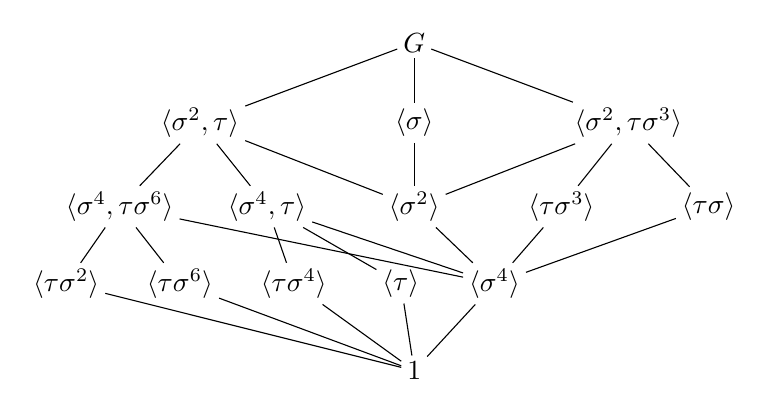
\begin{tikzpicture}[scale=0.85, baseline=(current bounding box.center), every node/.style={inner sep=2pt}]
\node (G) at (0,4.2) {$G$};
\node (a2t) at (-3.2,3.0) {$\langle\sigma^2,\tau\rangle$};
\node (a) at (0,3.0) {$\langle\sigma\rangle$};
\node (a2ta3) at (3.2,3.0) {$\langle\sigma^2,\tau\sigma^3\rangle$};
\node (a4ta6) at (-4.4,1.75) {$\langle\sigma^4,\tau\sigma^6\rangle$};
\node (a4t) at (-2.2,1.75) {$\langle\sigma^4,\tau\rangle$};
\node (a2) at (0,1.75) {$\langle\sigma^2\rangle$};
\node (ta3) at (2.2,1.75) {$\langle\tau\sigma^3\rangle$};
\node (ta) at (4.4,1.75) {$\langle\tau\sigma\rangle$};
\node (ta2) at (-5.2,0.6) {$\langle\tau\sigma^2\rangle$};
\node (ta6) at (-3.5,0.6) {$\langle\tau\sigma^6\rangle$};
\node (ta4) at (-1.8,0.6) {$\langle\tau\sigma^4\rangle$};
\node (t) at (-0.2,0.6) {$\langle\tau\rangle$};
\node (a4) at (1.2,0.6) {$\langle\sigma^4\rangle$};
\node (one) at (0,-0.7) {$1$};
\foreach \x in {a2t,a,a2ta3}{\draw (G)--(\x);}
\draw (a2t)--(a4ta6); \draw (a2t)--(a4t); \draw (a2t)--(a2);
\draw (a)--(a2);
\draw (a2ta3)--(a2); \draw (a2ta3)--(ta3); \draw (a2ta3)--(ta);
\draw (a4ta6)--(ta2); \draw (a4ta6)--(ta6); \draw (a4ta6)--(a4);
\draw (a4t)--(ta4); \draw (a4t)--(t); \draw (a4t)--(a4);
\draw (a2)--(a4);
\draw (ta3)--(a4); \draw (ta)--(a4);
\foreach \x in {ta2,ta6,ta4,t,a4}{\draw (\x)--(one);}
\end{tikzpicture}
\]

利用基本定理中 (2)——即在 $\mathbb Q$ 上的扩张次数等于固定子群的指数——对上面许多子群确定相应子域（根据基本定理，这给出了 $\mathbb Q(\sqrt[8]{2},i)$ 的所有子域）是相当简单的。于是只需找出一个具有正确次数、并被相应子群固定的子域。还要记住，如果一个子域被某个子群的生成元固定，那么它就被该子群固定。例如，从自同构 $\sigma$ 的显式描述可见，$\mathbb Q(i)$ 被 $\sigma$ 生成的群固定。由于这是指数为 $2$ 的子群，而 $\mathbb Q(i)$ 在 $\mathbb Q$ 上次数为 $2$，它必定就是全部固定域。上面大多数子群的固定域都可以这样简单地确定。

对右边的 $4$ 阶子群（即由 $\tau\sigma^3$ 与由 $\tau\sigma$ 生成的子群），也许不那么容易看出如何确定相应的固定域。对由 $\tau\sigma^3$ 生成的子群 $H$，可作如下处理：元素 $\theta^2=\sqrt[4]{2}$ 显然被 $\sigma^4$ 固定。由上面的图，$\sigma^4$ 是 $H$ 的一个指数为 $2$ 的正规子群，其陪集代表可取 $1,\tau\sigma^3$。考虑元素
\[
\alpha=(1+\tau\sigma^3)\theta^2=\theta^2+\tau\sigma^3\theta^2.
\]
那么 $\alpha$ 被 $\sigma^4$ 固定（我们在 $4$ 阶交换群 $H$ 中，所以 $\sigma^4$ 与 $1$、$\tau\sigma^3$ 交换，并且已经知道 $\theta^2$ 被 $\sigma^4$ 固定）。但是（这正是关键）$\alpha$ 也被 $\tau\sigma^3$ 固定：
\[
\tau\sigma^3\alpha=\tau\sigma^3(1+\tau\sigma^3)\theta^2=[\tau\sigma^3+(\tau\sigma^3)^2]\theta^2
=(\tau\sigma^3+\sigma^4)\theta^2,
\]
而最后这个表达式就是 $\alpha$，因为 $\sigma^4\theta^2=\theta^2$。因此 $\alpha$ 属于 $H$ 的固定域。显式地，
\[
\alpha=\sqrt[4]{2}+i\sqrt[4]{2}=(1+i)\sqrt[4]{2}.
\]
快速检查可见 $\alpha$ 不被自同构 $\sigma^2$ 固定，因此由上面的子群图可知，域 $\mathbb Q(\alpha)$ 的固定子群不可能大于 $H$，从而正是 $H$，这就给出了固定域。回忆一般地，如果 $E$ 是 $H$ 的固定域，那么 $\tau H\tau^{-1}$ 的固定域是 $\tau(E)$，这也给出了 $\langle\tau\sigma\rangle$ 的固定域。对 $H=\langle\tau\sigma^3\rangle$，有 $\tau H\tau^{-1}=\langle\tau\sigma\rangle$，其固定域由
\[
\tau(\alpha)=(1-i)\sqrt[4]{2}
\]
给出。

一般而言，人们试图确定被 Galois 群中给定子群 $H$ 固定的元素（参见练习，那里指出了上面的元素从何而来），并尝试生成足够大的域以得到全部固定域。在我们的情形中，我们能够用单个生成元做到这一点。稍后我们将看到，$\mathbb Q$ 的任意有限扩张都是单扩张，因此会有这种类型的单个生成元；不过一般而言可能难以直接产生它。

元素 $\alpha$ 是多项式
\[
x^4+8
\]
的根；这个多项式因此必定不可约，因为我们已经确定了它的一个根生成 $\mathbb Q$ 上次数为 $4$ 的扩张。

类似地，可以补全 $\mathbb Q(\sqrt[8]{2},i)$ 的子域图。为了强调它与上面子群图的关系，我们把它倒置过来（$\theta=\sqrt[8]{2}$）：
\[
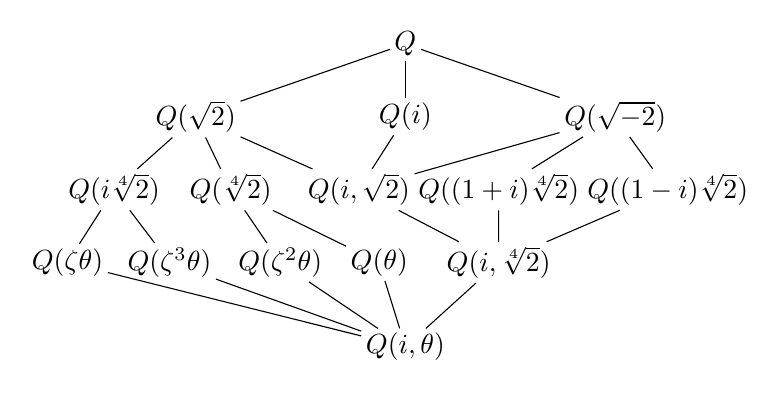
\begin{tikzpicture}[scale=0.74, baseline=(current bounding box.center), every node/.style={inner sep=1.5pt}]
\node (Q) at (0,4.4) {$\mathbb Q$};
\node (sqrt2) at (-3.6,3.15) {$\mathbb Q(\sqrt2)$};
\node (i) at (0,3.15) {$\mathbb Q(i)$};
\node (sqrtm2) at (3.6,3.15) {$\mathbb Q(\sqrt{-2})$};
\node (iq4) at (-5.0,1.9) {$\mathbb Q(i\sqrt[4]{2})$};
\node (q4) at (-3.0,1.9) {$\mathbb Q(\sqrt[4]{2})$};
\node (isqrt2) at (-0.8,1.9) {$\mathbb Q(i,\sqrt2)$};
\node (onep) at (1.6,1.9) {$\mathbb Q((1+i)\sqrt[4]{2})$};
\node (onem) at (4.5,1.9) {$\mathbb Q((1-i)\sqrt[4]{2})$};
\node (ztheta) at (-5.8,0.65) {$\mathbb Q(\zeta\theta)$};
\node (z3theta) at (-4.05,0.65) {$\mathbb Q(\zeta^3\theta)$};
\node (z2theta) at (-2.15,0.65) {$\mathbb Q(\zeta^2\theta)$};
\node (theta) at (-0.45,0.65) {$\mathbb Q(\theta)$};
\node (iq4full) at (1.6,0.65) {$\mathbb Q(i,\sqrt[4]{2})$};
\node (bottom) at (0,-0.8) {$\mathbb Q(i,\theta)$};
\draw (Q)--(sqrt2); \draw (Q)--(i); \draw (Q)--(sqrtm2);
\draw (sqrt2)--(iq4); \draw (sqrt2)--(q4); \draw (sqrt2)--(isqrt2);
\draw (i)--(isqrt2);
\draw (sqrtm2)--(isqrt2); \draw (sqrtm2)--(onep); \draw (sqrtm2)--(onem);
\draw (iq4)--(ztheta); \draw (iq4)--(z3theta); \draw (q4)--(z2theta); \draw (q4)--(theta); \draw (isqrt2)--(iq4full); \draw (onep)--(iq4full); \draw (onem)--(iq4full);
\foreach \x in {ztheta,z3theta,z2theta,theta,iq4full}{\draw (\x)--(bottom);}
\end{tikzpicture}
\]
注意，群 $\langle\sigma^4\rangle$ 是 $G$ 的正规子群（事实上是 $G$ 的中心），并且商群 $G/\langle\sigma^4\rangle\cong D_8$，所以相应固定域 $\mathbb Q(i,\sqrt[4]{2})$ 在 $\mathbb Q$ 上是 Galois 的，Galois 群为 $D_8$。由于它是 Galois 的，它是某个分裂域，显然是 $x^4-2$ 的分裂域。这个域的子域格于是立即由上面的格给出。

我们以这个 Galois 扩张的下列有趣方面结束这个例子。容易验证
\[
\langle\sigma^2,\tau\rangle\cong D_8,
\qquad
\langle\sigma\rangle\cong\mathbb Z/8\mathbb Z,
\qquad
\langle\sigma^2,\tau\sigma^3\rangle\cong Q_8,
\]
其中 $D_8$ 是 $8$ 阶二面体群，$Q_8$ 是 $8$ 阶四元数群。因此，域 $\mathbb Q(\sqrt[8]{2},i)$ 在它的三个二次子域
\[
\mathbb Q(\sqrt2),
\qquad
\mathbb Q(i),
\qquad
\mathbb Q(\sqrt{-2})
\]
上分别是次数为 $8$ 的 Galois 扩张，其 Galois 群分别为二面体群、循环群和四元数群。于是 $8$ 阶群的 $5$ 种可能类型中有三种（并且两个非交换的类型都）作为这个扩张中的 Galois 群出现。

我们将在下面各节考虑更多例子和应用。

\subsection*{练习}

\begin{enumerate}[label=\arabic*.]
\item 求元素 $\sqrt2+\sqrt5$ 在 $\mathbb Q$ 上的极小多项式。

\item 求元素 $1+\sqrt[3]{2}+\sqrt[3]{4}$ 在 $\mathbb Q$ 上的极小多项式。

\item 求 $(x^2-2)(x^2-3)(x^2-5)$ 的 Galois 群。求这个多项式的分裂域的所有子域。

\item 设 $p$ 为素数。求 $x^p-2$ 的 Galois 群的元素。

\item 证明：当 $p$ 为素数时，$x^p-2$ 的 Galois 群同构于矩阵群
\[
\left\{\begin{pmatrix}a&b\\0&1\end{pmatrix}\mid a,b\in\mathbb F_p,
\ a\neq0\right\}.
\]

\item 令 $K=\mathbb Q(\sqrt[8]{2},i)$，并令 $F_1=\mathbb Q(i)$、$F_2=\mathbb Q(\sqrt2)$、$F_3=\mathbb Q(\sqrt{-2})$。证明
\[
\operatorname{Gal}(K/F_1)\cong\mathbb Z_8,
\qquad
\operatorname{Gal}(K/F_2)\cong D_8,
\qquad
\operatorname{Gal}(K/F_3)\cong Q_8.
\]

\item 求 $x^8-2$ 的分裂域中所有在 $\mathbb Q$ 上 Galois 的子域。

\item 设 $K$ 是 $F$ 的一个次数为 $p^n$ 的 Galois 扩张，其中 $p$ 是素数且 $n\geq1$。证明在 $K$ 中存在 $F$ 的次数为 $p$ 和 $p^{n-1}$ 的 Galois 扩张。

\item 给出域 $F_1,F_2,F_3$ 的例子，使得 $\mathbb Q\subset F_1\subset F_2\subset F_3$，$[F_3:\mathbb Q]=8$，并且每个域都在其所有子域上是 Galois 的，唯一例外是 $F_2$ 不在 $\mathbb Q$ 上 Galois。

\item 求 $x^8-3$ 在 $\mathbb Q$ 上的分裂域的 Galois 群。

\item 设 $f(x)\in\mathbb Z[x]$ 是不可约四次多项式，并且它在 $\mathbb Q$ 上的分裂域的 Galois 群为 $S_4$（这样的四次多项式有很多，参见第 6 节）。令 $\theta$ 是 $f(x)$ 的一个根，并设 $K=\mathbb Q(\theta)$。证明 $K$ 是 $\mathbb Q$ 的次数为 $4$ 的扩张，并且没有真子域。是否存在次数为 $4$ 且没有真子域的 $\mathbb Q$ 的 Galois 扩张？

\item 求 $x^4-14x^2+9$ 在 $\mathbb Q$ 上的分裂域的 Galois 群。

\item 证明：如果某个三次多项式在 $\mathbb Q$ 上的分裂域的 Galois 群是 $3$ 阶循环群，那么该三次多项式的所有根都是实数。

\item 证明 $\mathbb Q(\sqrt{2+\sqrt2})$ 是一个循环四次域，即它是一个次数为 $4$ 且 Galois 群为循环群的 Galois 扩张。

\item （二二次扩张）设 $F$ 是一个特征不为 $2$ 的域。
\begin{enumerate}[label=(\alph*)]
\item 若 $K=F(\sqrt{D_1},\sqrt{D_2})$，其中 $D_1,D_2\in F$，并且 $D_1$、$D_2$、$D_1D_2$ 都不是 $F$ 中的平方，证明 $K/F$ 是 Galois 扩张，且 $\operatorname{Gal}(K/F)$ 同构于 Klein 四元群。
\item 反过来，设 $K/F$ 是 Galois 扩张，并且 $\operatorname{Gal}(K/F)$ 同构于 Klein 四元群。证明 $K=F(\sqrt{D_1},\sqrt{D_2})$，其中 $D_1,D_2\in F$，并且 $D_1$、$D_2$、$D_1D_2$ 都不是 $F$ 中的平方。
\end{enumerate}

\item
\begin{enumerate}[label=(\alph*)]
\item 证明 $x^4-2x^2-2$ 在 $\mathbb Q$ 上不可约。
\item 说明这个四次多项式的根为
\[
\alpha_1=\sqrt{1+\sqrt3},\quad
\alpha_2=\sqrt{1-\sqrt3},\quad
\alpha_3=-\sqrt{1+\sqrt3},\quad
\alpha_4=-\sqrt{1-\sqrt3}.
\]
\item 令 $K_1=\mathbb Q(\alpha_1)$、$K_2=\mathbb Q(\alpha_2)$。说明 $K_1\neq K_2$，且 $K_1\cap K_2=\mathbb Q(\sqrt3)=F$。
\item 证明 $K_1$、$K_2$ 和 $K_1K_2$ 都在 $F$ 上 Galois，并且 $\operatorname{Gal}(K_1K_2/F)$ 是 Klein 四元群。明确写出 $\operatorname{Gal}(K_1K_2/F)$ 的元素。确定 Galois 群的所有子群，并给出它们对应的含 $F$ 的 $K_1K_2$ 的固定子域。
\item 证明 $x^4-2x^2-2$ 在 $\mathbb Q$ 上的分裂域次数为 $8$，其 Galois 群为二面体群。
\end{enumerate}

下面两个练习指出了在给定域中构造子域元素的一种方法，并且在许多计算中相当有用。

\item 设 $K/F$ 是任意有限扩张，$\alpha\in K$。令 $L$ 是一个含有 $K$ 的 $F$ 的 Galois 扩张，并令 $H\leq\operatorname{Gal}(L/F)$ 是对应于 $K$ 的子群。定义 $\alpha$ 从 $K$ 到 $F$ 的\emph{范数}为
\[
N_{K/F}(\alpha)=\prod_\sigma \sigma(\alpha),
\]
其中乘积取遍 $K$ 到 $F$ 的一个代数闭包中的所有嵌入（所以由 Galois 理论基本定理，它取遍 $\operatorname{Gal}(L/F)$ 中 $H$ 的一组陪集代表）。这是 $\alpha$ 的 Galois 共轭的乘积。特别地，如果 $K/F$ 是 Galois 的，那么这是
\[
\prod_{\sigma\in\operatorname{Gal}(K/F)}\sigma(\alpha).
\]
\begin{enumerate}[label=(\alph*)]
\item 证明 $N_{K/F}(\alpha)\in F$。
\item 证明 $N_{K/F}(\alpha\beta)=N_{K/F}(\alpha)N_{K/F}(\beta)$，因此范数是从 $K$ 到 $F$ 的乘法映射。
\item 令 $K=F(\sqrt D)$ 是 $F$ 的一个二次扩张。说明
\[
N_{K/F}(a+b\sqrt D)=a^2-Db^2.
\]
\item 设
\[
m_\alpha(x)=x^d+a_{d-1}x^{d-1}+\cdots+a_1x+a_0\in F[x]
\]
是 $\alpha\in K$ 在 $F$ 上的极小多项式。令 $n=[K:F]$。证明 $d$ 整除 $n$，并且 $\alpha$ 的 $d$ 个互异 Galois 共轭在上面的乘积中都重复 $n/d$ 次，从而推出
\[
N_{K/F}(\alpha)=(-1)^n a_0^{n/d}.
\]
\end{enumerate}

\item 在前一题的记号下，定义 $\alpha$ 从 $K$ 到 $F$ 的\emph{迹}为
\[
\operatorname{Tr}_{K/F}(\alpha)=\sum_\sigma \sigma(\alpha),
\]
即 Galois 共轭的和。
\begin{enumerate}[label=(\alph*)]
\item 证明 $\operatorname{Tr}_{K/F}(\alpha)\in F$。
\item 证明
\[
\operatorname{Tr}_{K/F}(\alpha+\beta)=\operatorname{Tr}_{K/F}(\alpha)+\operatorname{Tr}_{K/F}(\beta),
\]
因此迹是从 $K$ 到 $F$ 的加法映射。
\item 令 $K=F(\sqrt D)$ 是 $F$ 的一个二次扩张。说明
\[
\operatorname{Tr}_{K/F}(a+b\sqrt D)=2a.
\]
\item 设 $m_\alpha(x)$ 如前一题所述。证明
\[
\operatorname{Tr}_{K/F}(\alpha)=-a_{d-1}.
\]
\end{enumerate}

\item 在前面各题的记号下，证明对基域 $F$ 中所有 $a$，有
\[
N_{K/F}(a\alpha)=a^nN_{K/F}(\alpha),
\qquad
\operatorname{Tr}_{K/F}(a\alpha)=a\operatorname{Tr}_{K/F}(\alpha).
\]
特别地，对所有 $a\in F$，证明
\[
N_{K/F}(a)=a^n,
\qquad
\operatorname{Tr}_{K/F}(a)=na.
\]

\item 在前面各题的记号下，更一般地证明
\[
\prod_\sigma (x-\sigma(\alpha))=(m_\alpha(x))^{n/d}.
\]

\item 利用特征的线性无关性证明：对任意 Galois 扩张 $K/F$，存在 $\alpha\in K$ 使得 $\operatorname{Tr}_{K/F}(\alpha)\neq0$。

\item 设 $K/F$ 是 Galois 扩张，$\sigma$ 是 Galois 群的一个元素。
\begin{enumerate}[label=(\alph*)]
\item 设 $\alpha\in K$ 具有形式
\[
\alpha=\frac{\beta}{\sigma\beta}
\]
其中 $0\neq\beta\in K$。证明 $N_{K/F}(\alpha)=1$。
\item 设 $\alpha\in K$ 具有形式
\[
\alpha=\beta-\sigma\beta
\]
其中 $\beta\in K$。证明 $\operatorname{Tr}_{K/F}(\alpha)=0$。
\end{enumerate}

下一题和后面的练习 26 建立 Hilbert 定理 90 的乘法形式与加法形式。这些是第一上同调群消失的例子，如第 17.3 节将讨论的那样。

\item （Hilbert 定理 90）设 $K$ 是 $F$ 的 Galois 扩张，其 Galois 群为由 $\sigma$ 生成的 $n$ 阶循环群。设 $\alpha\in K$ 满足 $N_{K/F}(\alpha)=1$。证明 $\alpha$ 具有形式
\[
\alpha=\frac{\beta}{\sigma\beta}
\]
其中 $0\neq\beta\in K$。[利用特征的线性无关性证明存在某个 $\theta\in K$ 使得
\[
\beta=\theta+\alpha\sigma(\theta)+(\alpha\sigma\alpha)\sigma^2(\theta)+\cdots+(
\alpha\sigma\alpha\cdots\sigma^{n-2}\alpha)\sigma^{n-1}(\theta)
\]
非零。利用 $\alpha$ 到 $F$ 的范数为 $1$ 这一事实计算 $\beta/\sigma\beta$。]

\item 证明 Pythagoras 方程 $a^2+b^2=1$ 的有理数解 $a,b\in\mathbb Q$ 具有形式
\[
a=\frac{s^2-t^2}{s^2+t^2},
\qquad
b=\frac{2st}{s^2+t^2}
\]
其中 $s,t\in\mathbb Q$；并由此说明任意整数边直角三角形的边长为
\[
(m^2-n^2,\ 2mn,\ m^2+n^2)
\]
其中 $m,n$ 是整数。[注意 $a^2+b^2=1$ 等价于 $N_{\mathbb Q(i)/\mathbb Q}(a+ib)=1$，然后把上面的 Hilbert 定理 90 用于 $\beta=s+it$。]

\item 将前一题推广，确定方程
\[
a^2+Db^2=1
\]
的所有有理数解，其中 $D\in\mathbb Z$，$D>0$，并且 $D$ 不是 $\mathbb Z$ 中的完全平方。

\item （加法 Hilbert 定理 90）设 $K$ 是 $F$ 的 Galois 扩张，其 Galois 群为由 $\sigma$ 生成的 $n$ 阶循环群。设 $\alpha\in K$ 满足 $\operatorname{Tr}_{K/F}(\alpha)=0$。证明 $\alpha$ 具有形式
\[
\alpha=\beta-\sigma\beta
\]
其中 $\beta\in K$。[由前一练习，取 $\theta\in K$ 满足 $\operatorname{Tr}_{K/F}(\theta)\neq0$，令
\[
\beta=\frac{1}{\operatorname{Tr}_{K/F}(\theta)}
\bigl[\alpha\sigma(\theta)+(\alpha+\sigma\alpha)\sigma^2(\theta)+\cdots+
(\alpha+\sigma\alpha+\cdots+\sigma^{n-2}\alpha)\sigma^{n-1}(\theta)\bigr]
\]
并计算 $\beta-\sigma\beta$。]

\item 令
\[
\alpha=\sqrt{(2+\sqrt2)(3+\sqrt3)}
\]
（为具体起见取正实平方根），并考虑扩张 $E=\mathbb Q(\alpha)$。
\begin{enumerate}[label=(\alph*)]
\item 说明 $\alpha^2=(2+\sqrt2)(3+\sqrt3)$ 不是 $F=\mathbb Q(\sqrt2,\sqrt3)$ 中的平方。[若 $\alpha^2=c^2$，$c\in F$，则对固定 $\mathbb Q(\sqrt2)$ 的自同构 $\varphi\in\operatorname{Gal}(F/\mathbb Q)$ 有
\[
\alpha\varphi(\alpha)=(2+\sqrt2)^2(6)=(c\varphi c)^2.
\]
由于 $c\varphi c=N_{F/\mathbb Q(\sqrt2)}(c)\in\mathbb Q(\sqrt2)$，推出这蕴含 $\sqrt6\in\mathbb Q(\sqrt2)$，矛盾。]
\item 由 (a) 推出 $[E:\mathbb Q]=8$。证明 $\alpha$ 在 $\mathbb Q$ 上的极小多项式的根是 $8$ 个元素
\[
\pm\sqrt{(2\pm\sqrt2)(3\pm\sqrt3)}.
\]
\item 令
\[
\beta=\sqrt{(2-\sqrt2)(3+\sqrt3)}.
\]
证明 $\alpha\beta=\sqrt2(3+\sqrt3)\in F$，因此 $\beta\in E$。类似地说明其他根也都属于 $E$，从而 $E$ 是 $\mathbb Q$ 的 Galois 扩张。说明 Galois 群的元素恰好是由把 $\alpha$ 映到 (b) 中八个元素之一所确定的映射。
\item 令 $\sigma\in\operatorname{Gal}(E/\mathbb Q)$ 为把 $\alpha$ 映到 $\beta$ 的自同构。说明由于 $\sigma(\alpha^2)=\beta^2$，有 $\sigma(\sqrt2)=-\sqrt2$ 且 $\sigma(\sqrt3)=\sqrt3$。由 $\alpha\beta=\sqrt2(3+\sqrt3)$ 推出 $\sigma(\alpha\beta)=-\alpha\beta$，从而 $\sigma(\beta)=-\alpha$。说明 $\sigma$ 是 $\operatorname{Gal}(E/\mathbb Q)$ 中的一个 $4$ 阶元素。
\item 类似地说明由
\[
\tau(\alpha)=\sqrt{(2+\sqrt2)(3-\sqrt3)}
\]
定义的映射 $\tau$ 是 $\operatorname{Gal}(E/\mathbb Q)$ 中的一个 $4$ 阶元素。证明 $\sigma$ 与 $\tau$ 生成 Galois 群，$\sigma^4=\tau^4=1$，$\sigma^2=\tau^2$，且 $\sigma\tau=\tau\sigma^3$。
\item 推出 $\operatorname{Gal}(E/\mathbb Q)\cong Q_8$，即 $8$ 阶四元数群。
\end{enumerate}

\item 设 $f(x)\in F[x]$ 是域 $F$ 上次数为 $n$ 的不可约多项式，$L$ 是 $f(x)$ 在 $F$ 上的分裂域，$\alpha$ 是 $f(x)$ 在 $L$ 中的一个根。若 $K$ 是 $F$ 的包含在 $L$ 中的任意 Galois 扩张，说明多项式 $f(x)$ 在 $K$ 上分解为 $m$ 个不可约多项式的乘积，每个不可约因子的次数为 $d$，其中
\[
m=[F(\alpha)\cap K:F],
\qquad
 d=[K(\alpha):K]
\]
（也参见第 4 节练习 4 中的推广）。[若 $H$ 是 $L/F$ 的 Galois 群中对应于 $K$ 的子群，则 $f(x)$ 在 $K$ 上的因子对应于 $H$ 在 $f(x)$ 的根上的轨道。然后使用第 4.1 节练习 9。]

\item 设 $k$ 是域，$k(t)$ 是变量 $t$ 中的有理函数域。定义 $k(t)$ 到自身的映射 $\sigma$ 与 $\tau$ 为
\[
\sigma f(t)=f\left(\frac{-1}{1-t}\right),
\qquad
\tau f(t)=f\left(\frac1t\right),
\qquad f(t)\in k(t).
\]
\begin{enumerate}[label=(\alph*)]
\item 证明 $\sigma$ 与 $\tau$ 是 $k(t)$ 的自同构（参见第 1 节练习 8），并且它们生成的群 $G=\langle\sigma,\tau\rangle$ 同构于 $S_3$。
\item 证明元素
\[
s=\frac{(t^2-t+1)^3}{t^2(t-1)^2}
\]
被 $G$ 的所有元素固定。
\item 证明 $k(s)$ 正是 $G$ 在 $k(t)$ 中的固定域。[计算扩张次数。]
\end{enumerate}

\item 证明前一题中由 $\tau$ 生成的自同构子群的固定域是
\[
k\left(t+\frac1t\right).
\]
证明由自同构 $\tau\sigma^2$（它把 $t$ 映到 $1-t$）生成的子群的固定域是 $k(t(1-t))$。求由 $\tau\sigma$ 生成的子群的固定域，以及由 $\sigma$ 生成的子群的固定域。

\item 设 $K$ 是 $F$ 的次数为 $n$ 的有限扩张。令 $\alpha$ 是 $K$ 的一个元素。
\begin{enumerate}[label=(\alph*)]
\item 证明 $\alpha$ 通过在 $K$ 上的左乘作用，给出 $K$ 的一个 $F$-线性变换 $T_\alpha$。
\item 证明 $\alpha$ 在 $F$ 上的极小多项式同线性变换 $T_\alpha$ 的极小多项式相同。
\item 证明迹 $\operatorname{Tr}_{K/F}(\alpha)$ 是由 $T_\alpha$ 定义的 $n\times n$ 矩阵的迹（这说明“迹”这个词的两种用法是一致的）。证明范数 $N_{K/F}(\alpha)$ 是 $T_\alpha$ 的行列式。
\end{enumerate}
\end{enumerate}

\section{有限域}

有限域 $\mathbb F$ 的特征为某个素数 $p$，因而是 $\mathbb F_p$ 上的一个有限维向量空间。如果维数为 $n$，即 $[\mathbb F:\mathbb F_p]=n$，则 $\mathbb F$ 恰有 $p^n$ 个元素。我们已经看到（在命题 13.37 之后），$\mathbb F$ 同构于多项式 $x^{p^n}-x$ 的分裂域，因此在同构意义下唯一。我们把阶为 $p^n$ 的有限域记为 $\mathbb F_{p^n}$。

域 $\mathbb F_{p^n}$ 在 $\mathbb F_p$ 上是 Galois 的，它的 Galois 群是由 Frobenius 自同构生成的 $n$ 阶循环群
\[
\operatorname{Gal}(\mathbb F_{p^n}/\mathbb F_p)=\langle \sigma_p\rangle\cong \mathbb Z/n\mathbb Z,
\]
其中
\[
\sigma_p(\alpha)=\alpha^p.
\]
这正是推论 6 后例 7 的内容。由基本定理，$\mathbb F_{p^n}$ 的每个子域对应于 $\mathbb Z/n\mathbb Z$ 的一个子群。因此，对 $n$ 的每个正因子 $d$，恰有一个在 $\mathbb F_p$ 上次数为 $d$ 的子域，即由阶为 $n/d$ 的子群 $\langle \sigma_p^d\rangle$ 固定的域，并且没有其他子域。这个域同构于 $\mathbb F_{p^d}$，即阶为 $p^d$ 的唯一有限域。

由于 Galois 群是 Abel 群，每个子群都是正规子群，所以每个子域 $\mathbb F_{p^d}$（其中 $d$ 是 $n$ 的一个因子）都在 $\mathbb F_p$ 上是 Galois 的（这也可由这些域本身就是分裂域这一事实直接看出）。此外，Galois 群 $\operatorname{Gal}(\mathbb F_{p^d}/\mathbb F_p)$ 由 $\sigma_p$ 在商群
\[
\operatorname{Gal}(\mathbb F_{p^n}/\mathbb F_p)/\langle \sigma_p^d\rangle
\]
中的像生成。如果仍把这个元素记作 $\sigma_p$，我们就重新得到扩张 $\mathbb F_{p^d}/\mathbb F_p$ 的 Frobenius 自同构。（不过要注意，$\sigma_p$ 在 $\operatorname{Gal}(\mathbb F_{p^n}/\mathbb F_p)$ 中阶为 $n$，而在 $\operatorname{Gal}(\mathbb F_{p^d}/\mathbb F_p)$ 中阶为 $d$。）

我们把这些结果概括为如下命题。

\noindent\textbf{命题 15.} 任意有限域都同构于某个 $\mathbb F_{p^n}$，其中 $p$ 是素数且 $n\geq 1$。域 $\mathbb F_{p^n}$ 是多项式 $x^{p^n}-x$ 在 $\mathbb F_p$ 上的分裂域，其 Galois 群是由 Frobenius 自同构 $\sigma_p$ 生成的 $n$ 阶循环群。$\mathbb F_{p^n}$ 的子域全都在 $\mathbb F_p$ 上是 Galois 的，并且同 $n$ 的因子 $d$ 一一对应；它们是域 $\mathbb F_{p^d}$，即 $\sigma_p^d$ 的固定域。

任意有限域的有限扩张的相应陈述，都是命题 15 的容易推论，并在练习中列出。

作为一个初等应用，我们得到整数多项式 $x^4+1\in\mathbb Z[x]$ 的如下结果。

\noindent\textbf{推论 16.} 不可约多项式 $x^4+1\in\mathbb Z[x]$ 模每个素数 $p$ 都可约。

\begin{proof}
考虑素数 $p$ 上的多项式 $x^4+1\in\mathbb F_p[x]$。如果 $p=2$，则 $x^4+1=(x+1)^4$，因此该多项式可约。现在假设 $p$ 为奇素数。由于 $p$ 模 $8$ 同余于 $1,3,5$ 或 $7$，而这些数的平方都模 $8$ 同余于 $1$，所以 $p^2-1$ 可被 $8$ 整除。因此 $x^{p^2-1}-1$ 可被 $x^8-1$ 整除。于是有整除关系
\[
x^4+1\mid x^8-1\mid x^{p^2-1}-1\mid x^{p^2}-x,
\]
这说明 $x^4+1$ 的所有根都是 $x^{p^2}-x$ 的根。（等价地，这些根被 Frobenius 自同构的平方 $\sigma_p^2$ 固定。）由于 $x^{p^2}-x$ 的根就是域 $\mathbb F_{p^2}$，由 $x^4+1$ 的任意一个根生成的扩张在 $\mathbb F_p$ 上的次数至多为 $2$，这意味着 $x^4+1$ 不可能在 $\mathbb F_p$ 上不可约。
\end{proof}

乘法群 $\mathbb F_{p^n}^{\times}$ 显然是一个域的乘法群的有限子群。由命题 9.18，它是循环群。如果 $\theta$ 是任意一个生成元，那么显然
\[
\mathbb F_{p^n}=\mathbb F_p(\theta).
\]
这证明了如下结果。

\noindent\textbf{命题 17.} 有限域 $\mathbb F_{p^n}$ 是单扩张。特别地，对每个 $n\geq 1$，在 $\mathbb F_p$ 上都存在次数为 $n$ 的不可约多项式。

上面我们已经把有限域 $\mathbb F_{p^n}$ 描述为多项式 $x^{p^n}-x$ 的分裂域。由前一命题，这个域也可以描述为 $\mathbb F_p[x]$ 的一个商，即由 $\theta$ 的极小多项式所定义的商。由于 $\theta$ 必然是 $x^{p^n}-x$ 的根，我们看到 $\theta$ 的极小多项式是 $x^{p^n}-x$ 的一个次数为 $n$ 的因子。

反过来，设 $p(x)$ 是任意一个次数为 $d$ 的不可约多项式，并且 $p(x)$ 整除 $x^{p^n}-x$。如果 $\alpha$ 是 $p(x)$ 的一个根，那么扩张 $\mathbb F_p(\alpha)$ 是 $\mathbb F_{p^n}$ 的一个次数为 $d$ 的子域。因此 $d$ 是 $n$ 的一个因子，并且由命题 15，这个扩张是 Galois 的（事实上就是扩张 $\mathbb F_{p^d}$），所以特别地，$p(x)$ 的所有根都包含在 $\mathbb F_p(\alpha)$ 中。

域 $\mathbb F_{p^n}$ 的元素正是 $x^{p^n}-x$ 的根。如果按照这些根在 $\mathbb F_p$ 上的极小多项式的次数 $d$，把这个多项式的因子 $x-\alpha$ 分组，就得到：

\noindent\textbf{命题 18.} 多项式 $x^{p^n}-x$ 正好是 $\mathbb F_p[x]$ 中所有不同的不可约多项式的乘积，其中这些不可约多项式的次数 $d$ 取遍 $n$ 的所有因子。

这个命题可以用来递归地产生 $\mathbb F_p$ 上的不可约多项式。例如，$\mathbb F_2$ 上的不可约二次多项式是
\[
\frac{x^4-x}{x(x-1)}
\]
的因子，于是得到唯一的多项式 $x^2+x+1$。类似地，这个域上的不可约三次多项式是
\[
\frac{x^8-x}{x(x-1)}=x^6+x^5+x^4+x^3+x^2+x+1
\]
的因子，它分解为两个三次多项式
\[
x^3+x+1\qquad\text{和}\qquad x^3+x^2+1.
\]
不可约四次多项式由 $x^{16}-x$ 除以 $x(x-1)$ 以及上面的不可约二次多项式 $x^2+x+1$ 后，再分解为不可约四次多项式而得：
\[
\frac{x^{16}-x}{x(x-1)(x^2+x+1)}
=(x^4+x^3+x^2+x+1)(x^4+x^3+1)(x^4+x+1).
\]

这给出了一种确定 $\mathbb F_p$ 上所有给定次数不可约多项式之乘积的方法。实践中，存在用于模 $p$ 分解多项式的有效算法，它们可以给出各个不可约多项式（见练习）。掌握不可约多项式之所以重要，是因为它们给出有限域 $\mathbb F_{p^n}$ 的一种便于显式计算的表示，即把它表示为商
\[
\mathbb F_p[x]/(f(x)),
\]
其中 $f(x)$ 是次数为 $n$ 的不可约多项式。

还要注意，由于有限域 $\mathbb F_{p^n}$ 在同构意义下唯一，$\mathbb F_p[x]$ 分别模任意两个次数为 $n$ 的不可约多项式所得的商域全都同构。如果 $f_1(x)$ 和 $f_2(x)$ 都是次数为 $n$ 的不可约多项式，那么 $f_2(x)$ 在域
\[
\mathbb F_{p^n}\cong \mathbb F_p[x]/(f_1(x))
\]
中完全分裂。如果把 $f_2(x)$ 的一个根记为 $\alpha(x)$（强调它在 $\mathbb F_p[x]/(f_1(x))$ 中是一个次数 $<n$ 的关于 $x$ 的多项式），则同构由
\[
\mathbb F_p[x]/(f_2(x))\longrightarrow \mathbb F_p[x]/(f_1(x)),
\qquad
x\longmapsto \alpha(x)
\]
给出（我们把第一个域中 $f_2(x)$ 的一个根映到第二个域中 $f_2(x)$ 的一个根）。例如，如果
\[
f_1(x)=x^4+x^3+1,
\qquad
f_2(x)=x^4+x+1
\]
是上面确定的 $\mathbb F_2$ 上两个不可约四次多项式，那么一个简单计算验证
\[
\alpha(x)=x^3+x^2
\]
是 $f_2(x)$ 在 $\mathbb F_{16}=\mathbb F_2[x]/(x^4+x^3+1)$ 中的一个根。于是有
\[
\mathbb F_2[x]/(x^4+x+1)\longrightarrow \mathbb F_2[x]/(x^4+x^3+1)\quad(\cong \mathbb F_{16}),
\qquad
x\longmapsto x^3+x^2.
\]

如果我们假定一个初等数论结果，就可以给出次数为 $n$ 的不可约多项式的个数公式。定义 Möbius $\mu$-函数为
\[
\mu(n)=
\begin{cases}
1, & n=1,\\
0, & \text{如果 } n \text{ 有平方因子},\\
(-1)^r, & \text{如果 } n \text{ 有 } r \text{ 个不同素因子}.
\end{cases}
\]
如果 $f(n)$ 是定义在所有正整数 $n$ 上的函数，并且
\[
F(n)=\sum_{d\mid n} f(d),\qquad n=1,2,\ldots,
\]
那么 Möbius 反演公式说，可以由 $F(n)$ 恢复 $f(n)$：
\[
f(n)=\sum_{d\mid n}\mu(d)F\left(\frac{n}{d}\right),\qquad n=1,2,\ldots.
\]
这是一个初等数论结果，我们在此直接采用。定义
\[
\psi(n)=\text{$\mathbb F_p[x]$ 中次数为 $n$ 的不可约多项式的个数}.
\]
在命题 18 中比较次数得到
\[
p^n=\sum_{d\mid n} d\psi(d).
\]
对 $f(n)=n\psi(n)$ 应用 Möbius 反演公式，得到
\[
n\psi(n)=\sum_{d\mid n}\mu(d)p^{n/d},
\]
从而给出 $\mathbb F_p$ 上次数为 $n$ 的不可约多项式的个数公式：
\[
\psi(n)=\frac1n\sum_{d\mid n}\mu(d)p^{n/d}.
\]
例如，在 $p=2,n=4$ 的情形中，
\[
\psi(4)=\frac14[\mu(1)2^4+\mu(2)2^2+\mu(4)2^1]
=\frac14(16-4+0)=3,
\]
与我们上面直接确定的结果一致。

我们已经看到
\[
\mathbb F_{p^m}\subseteq \mathbb F_{p^n}\quad\text{当且仅当}\quad m\mid n.
\]
特别地，给定任意两个有限域 $\mathbb F_{p^{n_1}}$ 和 $\mathbb F_{p^{n_2}}$，存在第三个有限域含有它们（的同构副本），即 $\mathbb F_{p^{n_1n_2}}$。这给出了这些域上的一个偏序，并允许我们考虑它们的并。由于这些域给出了 $\mathbb F_p$ 的全部有限扩张，我们看到所有 $\mathbb F_{p^n}$ 的并是 $\mathbb F_p$ 的一个代数闭包，在同构意义下唯一：
\[
\overline{\mathbb F_p}=\bigcup_{n\geq 1}\mathbb F_{p^n}.
\]
这给出了 $\mathbb F_p$ 的代数闭包的一个简单描述。

\subsection*{练习}

\begin{enumerate}
\item 在 $\mathbb Z[x]$ 和 $\mathbb F_2[x]$ 中把 $x^8-x$ 分解成不可约多项式的乘积。

\item 写出 $\mathbb F_4$ 和 $\mathbb F_9$ 的乘法表。

\item 证明代数闭域必定是无限域。

\item 构造含有 $16$ 个元素的有限域，并找出它的乘法群的一个生成元。有多少个这样的生成元？

\item 给出 $x^3-x+1$ 与 $x^3-x-1$ 在 $\mathbb F_3$ 上的分裂域之间的一个显式同构。

\item 设 $K=\mathbb Q(\theta)=\mathbb Q(\sqrt{D_1},\sqrt{D_2})$，其中 $D_1,D_2\in\mathbb Z$，是一个双二次扩张，并设
\[
\theta=a+b\sqrt{D_1}+c\sqrt{D_2}+d\sqrt{D_1D_2},
\]
其中 $a,b,c,d\in\mathbb Z$。证明 $\theta$ 在 $\mathbb Q$ 上的极小多项式 $m_\theta(x)$ 在 $\mathbb Q$ 上不可约且次数为 $4$，但模每个素数 $p$ 都可约。特别地，证明多项式 $x^4-10x^2+1$ 在 $\mathbb Z[x]$ 中不可约，但模每个素数都可约。[使用有限域上不存在双二次扩张这一事实。]

\item 证明对每个素数 $p$，$2,3,6$ 中至少有一个是 $\mathbb F_p$ 中的平方。推出多项式
\[
x^6-11x^4+36x^2-36=(x^2-2)(x^2-3)(x^2-6)
\]
模每个素数 $p$ 都有根，但在 $\mathbb Z$ 中没有根。

\item 确定多项式 $x^p-x-a$ 在 $\mathbb F_p$ 上的分裂域，其中 $a\neq 0$ 且 $a\in\mathbb F_p$。显式说明其 Galois 群是循环群。[证明 $\alpha\mapsto \alpha+1$ 是一个自同构。] 这样的扩张称为 Artin--Schreier 扩张（参见第 7 节练习 9）。

\item 令 $q=p^m$ 为素数 $p$ 的一个幂，并令 $\mathbb F_q=\mathbb F_{p^m}$ 为含有 $q$ 个元素的有限域。令 $\sigma_q=\sigma_p^m$ 为 Frobenius 自同构 $\sigma_p$ 的第 $m$ 次幂，称为 $q$-Frobenius 自同构。
\begin{enumerate}[label=(\alph*)]
\item 证明 $\sigma_q$ 固定 $\mathbb F_q$。
\item 证明 $\mathbb F_q$ 的任意次数为 $n$ 的有限扩张都是 $x^{q^n}-x$ 在 $\mathbb F_q$ 上的分裂域，因此在同构意义下唯一。
\item 证明 $\mathbb F_q$ 的任意次数为 $n$ 的有限扩张都是循环扩张，并以 $\sigma_q$ 为生成元。
\item 证明 $\mathbb F_q$ 的唯一次数为 $n$ 的扩张的子域与 $n$ 的因子 $d$ 一一对应。
\end{enumerate}

\item 证明 $n$ 整除 $\varphi(p^n-1)$。[观察 $\varphi(p^n-1)$ 是一个阶为 $p^n-1$ 的循环群的自同构群的阶。]

\item 证明 $x^{p^n}-x+1$ 只有在 $n=1$ 或 $n=p=2$ 时才可能在 $\mathbb F_p$ 上不可约。[注意如果 $\alpha$ 是一个根，则对任意 $a\in\mathbb F_{p^n}$，$\alpha+a$ 也是根。证明这蕴含 $\mathbb F_p(\alpha)$ 含有 $\mathbb F_{p^n}$，且 $[\mathbb F_p(\alpha):\mathbb F_{p^n}]=p$。]

\paragraph{Berlekamp 分解算法.} 下面的练习概述 Berlekamp 分解算法，用于分解 $\mathbb F_p[x]$ 中的多项式。这个算法的效率基于用 Euclidean 算法在 $\mathbb F_p[x]$ 中计算最大公因子的效率，以及用矩阵行化简算法解线性方程组的效率。

令 $f(x)\in\mathbb F_p[x]$ 是次数为 $n$ 的首一多项式，并设
\[
f(x)=p_1(x)p_2(x)\cdots p_k(x),
\]
其中 $p_1(x),p_2(x),\ldots,p_k(x)$ 是 $\mathbb F_p[x]$ 中不同的首一不可约多项式的幂。

\item 证明为了把 $f(x)$ 写成 $\mathbb F_p[x]$ 中不可约多项式的乘积，只要确定因子 $p_1(x),\ldots,p_k(x)$ 即可。[如果 $p(x)=q(x)^N\in\mathbb F_p[x]$，其中 $q(x)$ 是首一不可约多项式，说明可通过检查 $p$ 次幂并与导数计算最大公因子来确定 $q(x)$。]

\item 令 $g(x)\in\mathbb F_p[x]$ 为任意次数 $<n$ 的多项式。记 $R(h(x))$ 为 $h(x)$ 除以 $f(x)$ 后的余式。证明下面条件等价：
\begin{enumerate}[label=(\alph*)]
\item $R(g(x^p))=g(x)$。
\item $f(x)$ 整除
\[
[g(x)-0][g(x)-1]\cdots[g(x)-(p-1)].
\]
[使用 $g(x^p)=g(x)^p$ 以及 $x^p-x$ 在 $\mathbb F_p[x]$ 中的分解。]
\item 对 $i=1,2,\ldots,k$，$p_i(x)$ 整除 (b) 中的乘积。
\item 对每个 $i=1,2,\ldots,k$，存在 $s_i\in\mathbb F_p$ 使得 $p_i(x)$ 整除 $g(x)-s_i$，即
\[
g(x)=s_i\pmod{p_i(x)}.
\]
\end{enumerate}

\item 证明满足前一练习中等价条件的次数 $<n$ 的多项式 $g(x)$ 构成 $\mathbb F_p$ 上一个维数为 $k$ 的向量空间 $V$。[使用中国剩余定理处理 13(d) 中 $s_i$ 的 $p^k$ 种可能选择。]

\item 设
\[
g(x)=b_0+b_1x+\cdots+b_{n-1}x^{n-1}\in V.
\]
对 $j=0,1,\ldots,n-1$，令
\[
R(x^{jp})=a_{0,j}+a_{1,j}x+\cdots+a_{n-1,j}x^{n-1},
\]
并令 $A$ 为 $n\times n$ 矩阵
\[
A=\begin{pmatrix}
a_{0,0}&a_{0,1}&\cdots&a_{0,n-1}\\
a_{1,0}&a_{1,1}&\cdots&a_{1,n-1}\\
\vdots&\vdots& &\vdots\\
a_{n-1,0}&a_{n-1,1}&\cdots&a_{n-1,n-1}
\end{pmatrix}.
\]
证明练习 13 中条件 (a) 对 $g(x)\in V$ 来说等价于
\[
(A-I)B=0,
\tag{**}
\]
其中 $B$ 是以 $b_0,b_1,\ldots,b_{n-1}$ 为项的列矩阵。推出矩阵 $A-I$ 的秩为 $n-k$。注意，这已经足以判断 $f(x)$ 是否不可约，而无需实际确定因子。

\item 令 $g_1(x),g_2(x),\ldots,g_k(x)$ 为 (**) 的一组解基（也就是 $V$ 的一组基），其中可取 $g_1(x)=1$。从 $w(x)=f(x)$ 开始，对 $f(x)$ 已经算出的每个因子，计算最大公因子
\[
(w(x),g_i(x)-s),\qquad i=2,3,\ldots,k,\\quad s\in\mathbb F_p.
\]
注意由练习 13(d)，$f(x)$ 的每个因子 $p_i(x)$ 都整除某个这样的最大公因子。当已经确定了 $k$ 个两两互素的因子时，过程终止。

证明这个过程确实给出所有因子 $p_1(x),p_2(x),\ldots,p_k(x)$，也就是说，可以由这个过程分离出各个因子 $p_1(x),p_2(x),\ldots,p_k(x)$。证明如下：如果并非如此，则对两个因子，比如 $p_1(x)$ 与 $p_2(x)$，对每个 $i=1,2,\ldots,k$ 都存在 $s_i\in\mathbb F_p$，使得 $g_i(x)-s_i$ 同时被 $p_1(x)$ 和 $p_2(x)$ 整除。由中国剩余定理，选择 $g(x)\in V$ 满足
\[
g(x)=0\pmod{p_1(x)},\qquad g(x)=1\pmod{p_2(x)}.
\]
把 $g(x)=\sum_{i=1}^k c_i g_i(x)$ 写成 $V$ 的基的线性组合，并令 $s=\sum_{i=1}^k c_i s_i\in\mathbb F_p$。证明 $s=0\pmod{p_1(x)}$，从而 $s=0$；而 $s=1\pmod{p_2(x)}$，从而 $s=1$，矛盾。

\item 本练习按照前面练习概述的 Berlekamp 分解算法，确定
\[
f(x)=x^5+x^2+4x+6
\]
在 $\mathbb F_7[x]$ 中的分解。
\begin{enumerate}[label=(\alph*)]
\item 证明
\[
x^7=x^2+3x^3+6x^4\pmod{f(x)}.
\]
类似地计算 $x^{14},x^{21}$ 和 $x^{28}$ 模 $f(x)$（注意 $x^{14}$ 最容易通过把 $x^7$ 的结果平方再约化来计算，等等），并说明此时练习 15 中的矩阵 $A$ 为
\[
A=\begin{pmatrix}
0&6&0&4&2\\
0&0&3&0&2\\
0&1&6&3&1\\
0&3&4&3&1\\
0&6&1&4&1
\end{pmatrix}.
\]
\item 说明 $A-I$ 的简化行阶梯形矩阵为
\[
\begin{pmatrix}
1&0&0&6&6\\
0&1&0&1&0\\
0&0&1&1&6\\
0&0&0&0&0\\
0&0&0&0&0
\end{pmatrix}.
\]
推出 $k=2$（所以 $f(x)$ 正好是两个因子的乘积，每个因子都是不可约多项式的幂），并且 $g_1(x)=1$ 与
\[
g_2(x)=x^4+5x^3+x^2+x
\]
给出练习 15 中 (**) 的解空间的一组基。
\item 按照练习 16 中的过程，证明
\[
(f(x),g_2(x)-1)=x^2+3x+5=p_1(x),
\]
且 $f(x)/p_1(x)=x^3+4x^2+4x+4=p_2(x)$，这给出 $\mathbb F_7[x]$ 中整除 $f(x)$ 的不可约多项式的幂。说明这两个因子都不是 $\mathbb F_7[x]$ 中的 $7$ 次幂，并且每个都与它的导数互素，从而推出二者都是不可约多项式，得到 $f(x)$ 到不可约多项式的完整分解
\[
f(x)=(x^2+3x+5)(x^3+4x^2+4x+4)\in\mathbb F_7[x].
\]
\end{enumerate}
\end{enumerate}

\section{复合扩张与单扩张}

现在我们考虑同 Galois 扩张取复合的效果。第一个结果说明，把一个 Galois 扩张“上滑”仍得到一个 Galois 扩张。

\noindent\textbf{命题 19.} 设 $K/F$ 是 Galois 扩张，$F'/F$ 是任意扩张。则 $KF'/F'$ 是 Galois 扩张，其 Galois 群
\[
\operatorname{Gal}(KF'/F')\cong \operatorname{Gal}(K/K\cap F')
\]
同构于 $\operatorname{Gal}(K/F)$ 的一个子群。图示为：
\[
\begin{tikzpicture}[scale=1.0, baseline=(current bounding box.center), every node/.style={inner sep=2pt}]
\node (top) at (0,2.1) {$KF'$};
\node (left) at (-1.6,0.7) {$K$};
\node (right) at (1.6,0.7) {$F'$};
\node (mid) at (0,-0.8) {$K\cap F'$};
\node (bot) at (0,-2.1) {$F$};
\draw (top)--(left);
\draw (top)--(right);
\draw (left)--(mid);
\draw (right)--(mid);
\draw (mid)--(bot);
\end{tikzpicture}
\]

\begin{proof}
如果 $K/F$ 是 Galois 的，则 $K$ 是 $F[x]$ 中某个可分多项式 $f(x)$ 的分裂域。于是 $KF'/F'$ 是把 $f(x)$ 视作 $F'[x]$ 中多项式时的分裂域，因此这个扩张是 Galois 的。由于 $K/F$ 是 Galois 的，固定 $F$ 的 $K$ 的每个嵌入都是 $K$ 的自同构，所以映射
\[
\varphi:\operatorname{Gal}(KF'/F')\longrightarrow \operatorname{Gal}(K/F),
\qquad
\sigma\longmapsto \sigma|_K
\]
由把自同构 $\sigma$ 限制到子域 $K$ 来定义，并且是良定义的。它显然是同态，其核为
\[
\ker\varphi=\{\sigma\in\operatorname{Gal}(KF'/F')\mid \sigma|_K=1\}.
\]
由于 $\operatorname{Gal}(KF'/F')$ 中的元素在 $F'$ 上平凡，核中的元素在 $K$ 和 $F'$ 上都平凡，因此在它们的复合上也平凡，所以核只含恒等自同构。因此 $\varphi$ 是单射。

令 $H$ 表示 $\varphi$ 在 $\operatorname{Gal}(K/F)$ 中的像，令 $K_H$ 表示 $K$ 中对应的、含有 $F$ 的固定子域。由于 $H$ 中的每个元素都固定 $F'$，$K_H$ 含有 $K\cap F'$。另一方面，复合 $K_HF'$ 被 $\operatorname{Gal}(KF'/F')$ 固定（任意 $\sigma\in\operatorname{Gal}(KF'/F')$ 固定 $F'$，并且在 $K_H\subseteq K$ 上按它的限制 $\sigma|_K\in H$ 作用，而后者按定义固定 $K_H$）。由基本定理可知 $K_HF'=F'$，所以 $K_H\subseteq F'$，这给出反向包含 $K_H\subseteq K\cap F'$。因此 $K_H=K\cap F'$，再由基本定理得到 $H=\operatorname{Gal}(K/K\cap F')$，证明完成。
\end{proof}

\noindent\textbf{推论 20.} 设 $K/F$ 是 Galois 扩张，$F'/F$ 是任意有限扩张。则
\[
[KF':F]=\frac{[K:F][F':F]}{[K\cap F':F]}.
\]

\begin{proof}
这由命题以及等式 $[KF':F']=[K:K\cap F']$ 得出，而这个等式由命题中 Galois 群的阶给出。
\end{proof}

例子 $F=\mathbb Q$，$K=\mathbb Q(\sqrt[3]{2})$，$F'=\mathbb Q(\rho\sqrt[3]{2})$，其中 $\rho$ 是一个本原三次单位根，说明如果两个扩张中没有一个是 Galois 的，那么推论 20 的公式一般不成立。

\noindent\textbf{命题 21.} 令 $K_1$ 和 $K_2$ 为域 $F$ 的 Galois 扩张。则
\begin{enumerate}[label=(\arabic*)]
\item 交 $K_1\cap K_2$ 在 $F$ 上是 Galois 的；
\item 复合 $K_1K_2$ 在 $F$ 上是 Galois 的。其 Galois 群同构于直积
\[
\operatorname{Gal}(K_1/F)\times\operatorname{Gal}(K_2/F)
\]
的子群
\[
H=\{(\sigma,\tau)\mid \sigma|_{K_1\cap K_2}=\tau|_{K_1\cap K_2}\},
\]
也就是限制到交 $K_1\cap K_2$ 上相等的那些元素组成的子群。
\end{enumerate}
\[
\begin{tikzpicture}[scale=1.0, baseline=(current bounding box.center), every node/.style={inner sep=2pt}]
\node (top) at (0,2.0) {$K_1K_2$};
\node (left) at (-1.5,0.7) {$K_1$};
\node (right) at (1.5,0.7) {$K_2$};
\node (mid) at (0,-0.8) {$K_1\cap K_2$};
\node (bot) at (0,-2.1) {$F$};
\draw (top)--(left);
\draw (top)--(right);
\draw (left)--(mid);
\draw (right)--(mid);
\draw (mid)--(bot);
\end{tikzpicture}
\]

\begin{proof}
(1) 设 $p(x)$ 是 $F[x]$ 中一个不可约多项式，并且在 $K_1\cap K_2$ 中有一个根 $\alpha$。由于 $\alpha\in K_1$ 且 $K_1/F$ 是 Galois 的，$p(x)$ 的所有根都在 $K_1$ 中。同理，所有根都在 $K_2$ 中，因此 $p(x)$ 的所有根都在 $K_1\cap K_2$ 中。由定理 13 中的判别可以容易地推出 $K_1\cap K_2$ 是 Galois 的。

(2) 如果 $K_1$ 是可分多项式 $f_1(x)$ 的分裂域，而 $K_2$ 是可分多项式 $f_2(x)$ 的分裂域，那么复合就是多项式 $f_1(x)f_2(x)$ 的无平方因子部分的分裂域，因此在 $F$ 上是 Galois 的。

映射
\[
\varphi:\operatorname{Gal}(K_1K_2/F)\longrightarrow
\operatorname{Gal}(K_1/F)\times\operatorname{Gal}(K_2/F),
\qquad
\sigma\longmapsto (\sigma|_{K_1},\sigma|_{K_2})
\]
显然是同态。其核由同时在 $K_1$ 与 $K_2$ 上平凡的元素 $\sigma$ 组成，因此在复合上平凡，所以这个映射是单射。它的像位于子群 $H$ 中，因为
\[
(\sigma|_{K_1})|_{K_1\cap K_2}=\sigma|_{K_1\cap K_2}=(\sigma|_{K_2})|_{K_1\cap K_2}.
\]

子群 $H$ 的阶可以这样计算：对每个 $\sigma\in\operatorname{Gal}(K_1/F)$，有 $|\operatorname{Gal}(K_2/K_1\cap K_2)|$ 个 $\tau\in\operatorname{Gal}(K_2/F)$，其在 $K_1\cap K_2$ 上的限制等于 $\sigma|_{K_1\cap K_2}$。因此
\[
\begin{aligned}
|H|&=|\operatorname{Gal}(K_1/F)|\cdot |\operatorname{Gal}(K_2/K_1\cap K_2)|\\
&=|\operatorname{Gal}(K_1/F)|\frac{|\operatorname{Gal}(K_2/F)|}{|\operatorname{Gal}(K_1\cap K_2/F)|}.
\end{aligned}
\]
由推论 20 和上图可知，$H$ 与 $\operatorname{Gal}(K_1K_2/F)$ 的阶都等于
\[
[K_1K_2:F]=\frac{[K_1:F][K_2:F]}{[K_1\cap K_2:F]}.
\]
因此 $\varphi$ 的像恰好就是 $H$，证明完成。
\end{proof}

\noindent\textbf{推论 22.} 令 $K_1$ 和 $K_2$ 为域 $F$ 的 Galois 扩张，并且 $K_1\cap K_2=F$。则
\[
\operatorname{Gal}(K_1K_2/F)\cong \operatorname{Gal}(K_1/F)\times\operatorname{Gal}(K_2/F).
\]
反过来，如果 $K$ 在 $F$ 上是 Galois 的，且
\[
G=\operatorname{Gal}(K/F)=G_1\times G_2
\]
是两个子群 $G_1$ 和 $G_2$ 的直积，那么 $K$ 是 $F$ 的两个 Galois 扩张 $K_1$ 和 $K_2$ 的复合，并且 $K_1\cap K_2=F$。

\begin{proof}
第一部分立即由命题推出。对于第二部分，令 $K_1$ 为 $G_1\subset G$ 的固定域，令 $K_2$ 为 $G_2\subset G$ 的固定域。那么 $K_1\cap K_2$ 对应于子群 $G_1G_2$，在此情形中它就是整个 $G$，所以 $K_1\cap K_2=F$。复合 $K_1K_2$ 对应于子群 $G_1\cap G_2$，这里它是恒等子群，所以 $K_1K_2=K$，证明完成。
\end{proof}

\noindent\textbf{推论 23.} 令 $E/F$ 为任意有限可分扩张。则 $E$ 包含在某个在 $F$ 上 Galois 的扩张 $K$ 中，并且 $K$ 是极小的，意思是在 $K$ 的一个固定代数闭包中，任何含有 $E$ 的 $F$ 的 Galois 扩张都含有 $K$。

\begin{proof}
存在一个含有 $E$ 的 $F$ 的 Galois 扩张，例如取 $E$ 在 $F$ 上一组基的极小多项式的分裂域的复合（由于 $E$ 在 $F$ 上可分，这些多项式都是可分的）。于是所有含有 $E$ 的 $F$ 的 Galois 扩张的交就是这个域 $K$。
\end{proof}

\noindent\textbf{定义.} 前一推论中含有 $E$ 的 $F$ 的 Galois 扩张 $K$ 称为 $E$ 在 $F$ 上的 \emph{Galois 闭包}。

在 Galois 扩张中工作通常更简单（例如在按推论 20 计算次数时）。可分扩张的 Galois 闭包的存在性，经常可用来把计算化归为对 Galois 扩张的考虑。

回忆：如果 $K=F(\theta)$ 对某个元素 $\theta$ 成立，则称 $F$ 的扩张 $K$ 是\emph{单}的，在这种情形下 $\theta$ 称为 $K$ 的一个本原元。

\noindent\textbf{命题 24.} 令 $K/F$ 为有限扩张。则 $K=F(\theta)$ 当且仅当含有 $F$ 的 $K$ 的子域只有有限多个。

\begin{proof}
首先假设 $K=F(\theta)$ 是单的。令 $E$ 为 $K$ 的一个含有 $F$ 的子域：$F\subseteq E\subseteq K$。令 $f(x)\in F[x]$ 为 $\theta$ 在 $F$ 上的极小多项式，令 $g(x)\in E[x]$ 为 $\theta$ 在 $E$ 上的极小多项式。则 $g(x)$ 在 $E[x]$ 中整除 $f(x)$。令 $E'$ 为 $g(x)$ 的系数在 $F$ 上生成的域。那么 $E'\subseteq E$，并且显然 $\theta$ 在 $E'$ 上的极小多项式仍为 $g(x)$。于是
\[
[K:E]=\deg g(x)=[K:E']
\]
蕴含 $E=E'$。因此，含有 $F$ 的 $K$ 的子域是由 $f(x)$ 的首一因子的系数生成的子域，从而这种子域只有有限多个。

反过来，假设含有 $F$ 的 $K$ 的子域只有有限多个。如果 $F$ 是有限域，那么我们已经看到 $K$ 是一个单扩张（命题 17）。因此可以假设 $F$ 是无限的。因为 $K$ 在 $F$ 上有限生成，显然只需证明 $F(\alpha,\beta)$ 由一个元素生成。考虑子域
\[
F(\alpha+c\beta),\qquad c\in F.
\]
由于 $F$ 中 $c$ 有无限多个选择，而这种子域只有有限多个，存在 $F$ 中的 $c,c'$，$c\neq c'$，使得
\[
F(\alpha+c\beta)=F(\alpha+c'\beta).
\]
于是 $\alpha+c\beta$ 和 $\alpha+c'\beta$ 都属于 $F(\alpha+c\beta)$，取它们的差可知 $(c-c')\beta\in F(\alpha+c\beta)$。因此 $\beta\in F(\alpha+c\beta)$，于是也有 $\alpha\in F(\alpha+c\beta)$。所以
\[
F(\alpha,\beta)\subseteq F(\alpha+c\beta),
\]
而反向包含显然成立，于是
\[
F(\alpha,\beta)=F(\alpha+c\beta),
\]
证明完成。
\end{proof}

\noindent\textbf{定理 25（本原元定理）.} 如果 $K/F$ 是有限且可分的，则 $K/F$ 是单扩张。特别地，特征为 $0$ 的域的任意有限扩张都是单扩张。

\begin{proof}
令 $L$ 为 $K$ 在 $F$ 上的 Galois 闭包。则含有 $F$ 的 $K$ 的任意子域，都由基本定理对应于 Galois 群 $\operatorname{Gal}(L/F)$ 的一个子群。由于这样的子群只有有限多个，前一命题说明 $K/F$ 是单的。最后一句话则由特征为 $0$ 的域的任意有限扩张都是可分的推出。
\end{proof}

如命题的证明所表明的，一个扩张的本原元可以取为该扩张的生成元的一个简单线性组合。在 Galois 扩张的情形中，只需确定一个不被 Galois 群的任何非平凡元素固定的线性组合，因为此时由基本定理，这个线性组合不可能属于任何真子域。

\paragraph{例}
\begin{enumerate}[label=(\arabic*)]
\item 元素 $\sqrt2+\sqrt3$ 生成域 $\mathbb Q(\sqrt2,\sqrt3)$，正如我们已经看到的那样（它不被这个域的四个 Galois 自同构中的任何一个固定）。
\item 有理函数域 $\overline{\mathbb F}_p(x,y)$，其中变量 $x$ 与 $y$ 取系数于 $\mathbb F_p$ 的代数闭包 $\overline{\mathbb F}_p$，不是子域
\[
F=\overline{\mathbb F}_p(x^p,y^p)
\]
的一个单扩张。容易看出
\[
[\overline{\mathbb F}_p(x,y):\overline{\mathbb F}_p(x^p,y^p)]=p^2,
\]
并且子域
\[
F(x+cy),\qquad c\in\overline{\mathbb F}_p
\]
都在 $\overline{\mathbb F}_p(x^p,y^p)$ 上次数为 $p$（注意 $(x+cy)^p=x^p+c^py^p\in\overline{\mathbb F}_p(x^p,y^p)$）。如果其中任意两个子域相等，那么正如命题 24 的证明中一样，我们会得到
\[
\overline{\mathbb F}_p(x,y)=F(x+cy),
\]
这由次数考虑是不可能的。因此存在无限多个这样的子域，并且这个扩张不是单扩张。
\end{enumerate}

\subsection*{练习}
\begin{enumerate}[label=\arabic*.]
\item 求域 $\mathbb Q(\sqrt{1+\sqrt2})$ 在 $\mathbb Q$ 上的 Galois 闭包。

\item 找出 $\mathbb Q(\sqrt2,\sqrt3,\sqrt5)$ 在 $\mathbb Q$ 上的一个本原生成元。

\item 令 $F$ 为包含在 $\mathbb Q$ 上 $n\times n$ 矩阵环中的一个域。证明 $[F:\mathbb Q]\leq n$。（注意，由第 13.2 节练习 19，$\mathbb Q$ 上 $n\times n$ 矩阵环确实含有次数为 $n$ 的 $\mathbb Q$ 上域。）

\item 设 $f(x)\in F[x]$ 是域 $F$ 上次数为 $n$ 的不可约多项式，$L$ 为 $f(x)$ 在 $F$ 上的分裂域，$\alpha$ 为 $f(x)$ 在 $L$ 中的一个根。如果 $K$ 是 $F$ 的任意 Galois 扩张，证明 $f(x)$ 在 $K$ 上分解为 $m$ 个次数均为 $d$ 的不可约多项式的乘积，其中
\[
d=[K(\alpha):K]=[(L\cap K)(\alpha):L\cap K],
\]
并且
\[
m=n/d=[F(\alpha)\cap K:F].
\]
[先证明 $f(x)$ 在 $K$ 上的分解与它在 $L\cap K$ 上的分解相同。然后，若 $H$ 是 $L$ 在 $F$ 上的 Galois 群中对应于 $L\cap K$ 的子群，则 $f(x)$ 在 $L\cap K$ 上的因子对应于 $H$ 在 $f(x)$ 的根上的轨道。使用第 4.1 节练习 9。]

\item 令 $p$ 为素数，$F$ 为一个域。令 $K$ 为 $F$ 的一个 Galois 扩张，其 Galois 群是一个 $p$-群（即次数 $[K:F]$ 是 $p$ 的幂）。这样的扩张称为一个 $p$-扩张（注意，$p$-扩张按定义是 Galois 的）。
\begin{enumerate}[label=(\alph*)]
\item 设 $L$ 是 $K$ 的一个 $p$-扩张。证明 $L$ 在 $F$ 上的 Galois 闭包是 $F$ 的一个 $p$-扩张。
\item 举例说明：如果 $[K:F]$ 是 $p$ 的幂但 $K/F$ 不是 Galois 的，则 (a) 不必成立。
\end{enumerate}

\item 通过明确展示无限多个中间子域，证明 $\overline{\mathbb F}_p(x,y)/\overline{\mathbb F}_p(x^p,y^p)$ 不是单扩张。

\item 设 $F\subseteq K\subseteq L$，且 $\theta\in L$，其中 $p(x)=m_{\theta,F}(x)$。证明作为 $K$-代数，
\[
K\otimes_F F(\theta)\cong K[x]/(p(x)).
\]

\item 设 $K_1$ 与 $K_2$ 是域 $F$ 的两个代数扩张，它们都包含在特征为零的域 $L$ 中。证明 $F$-代数 $K_1\otimes_F K_2$ 没有非零幂零元。[使用前一练习。]
\end{enumerate}

\section{分圆扩张与 $\mathbb Q$ 上的 Abel 扩张}

我们已经确定，$n$ 次单位根的分圆域 $\mathbb Q(\zeta_n)$ 是 $\mathbb Q$ 的一个 Galois 扩张，其次数为 $\varphi(n)$，其中 $\varphi$ 表示 Euler $\varphi$-函数。这个域的任一自同构都由它在本原 $n$ 次单位根 $\zeta_n$ 上的作用唯一决定。这个元素必须被映到另一个本原 $n$ 次单位根（回忆这些根就是不可约分圆多项式 $\Phi_n(x)$ 的根）。因此
\[
\sigma(\zeta_n)=\zeta_n^a
\]
对某个整数 $a$ 成立，其中 $1\leq a<n$，且 $a$ 与 $n$ 互素。由于这样的整数 $a$ 恰有 $\varphi(n)$ 个，于是事实上这些映射中的每一个都确实是 $\mathbb Q(\zeta_n)$ 的一个自同构。还要注意，对任意与 $n$ 互素的整数 $a$，我们都可以用同一个公式定义 $\sigma_a$，并且 $\sigma_a$ 只依赖于 $a$ 模 $n$ 的剩余类。

\noindent\textbf{定理 26.} $n$ 次单位根的分圆域 $\mathbb Q(\zeta_n)$ 的 Galois 群同构于乘法群 $(\mathbb Z/n\mathbb Z)^\times$。这个同构明确由映射
\[
(\mathbb Z/n\mathbb Z)^\times\longrightarrow \operatorname{Gal}(\mathbb Q(\zeta_n)/\mathbb Q),
\qquad
 a\pmod n\longmapsto \sigma_a
\]
给出，其中 $\sigma_a$ 是由
\[
\sigma_a(\zeta_n)=\zeta_n^a
\]
定义的自同构。

\begin{proof}
上面的讨论表明，对任意 $a\pmod n$，$\sigma_a$ 都是一个自同构，所以此映射良定义。它是同态，因为
\[
(\sigma_a\sigma_b)(\zeta_n)=\sigma_a(\zeta_n^b)=(\zeta_n^a)^b=\zeta_n^{ab},
\]
这说明 $\sigma_a\sigma_b=\sigma_{ab}$。由上面的讨论，这个映射是双射，因为我们知道每个 Galois 自同构都形如 $\sigma_a$，其中 $a\pmod n$ 唯一确定。因此这个映射是同构。
\end{proof}

\paragraph{例}
\begin{enumerate}[label=(\arabic*)]
\item 域 $\mathbb Q(\zeta_5)$ 在 $\mathbb Q$ 上是 Galois 的，其 Galois 群
\[
(\mathbb Z/5\mathbb Z)^\times\cong \mathbb Z/4\mathbb Z.
\]
这是我们第一个次数为 $4$ 且 Galois 群为循环群的 $\mathbb Q$ 的 Galois 扩张例子。按照上面的记号，Galois 群的元素是 $\{\sigma_1=1,\sigma_2,\sigma_3,\sigma_4\}$。这个循环群的一个生成元是
\[
\sigma_2:\zeta_5\longmapsto \zeta_5^2
\]
（因为 $2$ 在 $(\mathbb Z/5\mathbb Z)^\times$ 中有阶 $4$）。

这里只有一个非平凡子域，它是 $\mathbb Q$ 的一个二次扩张，即子群 $\{1,\sigma_4=\sigma_{-1}\}$ 的固定域。这个子域中的一个元素由
\[
\alpha=\zeta_5+\sigma_{-1}\zeta_5=\zeta_5+\zeta_5^{-1}
\]
给出，因为这个元素显然被 $\sigma_{-1}$ 固定。元素 $\zeta_5$ 满足
\[
\zeta_5^4+\zeta_5^3+\zeta_5^2+\zeta_5+1=0.
\]
于是注意到
\[
\begin{aligned}
\alpha^2+\alpha-1
&=(\zeta_5^2+2+\zeta_5^{-2})+(\zeta_5+\zeta_5^{-1})-1\\
&=\zeta_5^2+2+\zeta_5^3+\zeta_5+\zeta_5^4-1=0.
\end{aligned}
\]
显式解出 $\alpha$，可知由 $\alpha$ 生成的 $\mathbb Q$ 的二次扩张就是 $\mathbb Q(\sqrt 5)$：
\[
\mathbb Q(\zeta_5+\zeta_5^{-1})=\mathbb Q(\sqrt 5).
\]
一般可以证明（这并不完全平凡）：若 $p$ 是奇素数，则域 $\mathbb Q(\zeta_p)$ 含有二次域 $\mathbb Q(\sqrt{\pm p})$，其中当 $p\equiv 1\pmod 4$ 时取正号，当 $p\equiv 3\pmod 4$ 时取负号（参见第 13.6 节中的练习）。

\item 对 $\mathbb Q(\zeta_{13})$，并且更一般地，对奇素数 $p$，我们可以像前一个例子那样为 $\mathbb Q(\zeta_p)$ 的任意子域构造一个本原元。$\mathbb Q(\zeta_p)$ 在 $\mathbb Q$ 上的一组基为
\[
1,\zeta_p,\zeta_p^2,\ldots,\zeta_p^{p-2}.
\]
由于
\[
\zeta_p^{p-1}+\zeta_p^{p-2}+\cdots+\zeta_p+1=0,
\]
我们看到这些元素
\[
\zeta_p,\zeta_p^2,\ldots,\zeta_p^{p-2},\zeta_p^{p-1}
\]
也构成一组基。选择这组基的原因在于，Galois 群 $\operatorname{Gal}(\mathbb Q(\zeta_p)/\mathbb Q)$ 中的任意 $\sigma$ 都只是置换这些基元素，因为它们正是本原 $p$ 次单位根。注意，正是在这一点上我们需要 $p$ 是素数；一般地，本原 $n$ 次单位根并不构成 $n$ 次单位根分圆域在 $\mathbb Q$ 上的一组基（例如，本原 $4$ 次单位根 $\pm i$ 就不是线性无关的）。

令 $H$ 为 $\mathbb Q(\zeta_p)$ 在 $\mathbb Q$ 上的 Galois 群的任意子群，并令
\[
\alpha_H=\sum_{\sigma\in H}\sigma\zeta_p, \tag{14.10}
\]
即 $\zeta_p$ 在 $H$ 的元素下的共轭之和。对任意 $\tau\in H$，当 $\sigma$ 遍历 $H$ 时，元素 $\tau\sigma$ 也遍历 $H$。因此 $\tau\alpha=\alpha$，所以 $\alpha$ 位于 $H$ 的固定域中。若现在 $\tau$ 不是 $H$ 的元素，那么 $\tau\alpha$ 是若干基元素之和（回忆这里任意自同构都置换这些基元素），其中一项是 $\tau(\zeta_p)$。若有 $\tau\alpha=\alpha$，则由于这些元素构成一组基，我们必须有 $\tau(\zeta_p)=\sigma(\zeta_p)$，其中 $\sigma\zeta_p$ 是式 (10) 中的一项。但这意味着 $\tau\sigma^{-1}=1$，因为这个自同构在 $\zeta_p$ 上是恒等的。于是 $\tau=\sigma\in H$，矛盾。这说明 $\alpha$ 不被任何不属于 $H$ 的自同构固定，所以 $\mathbb Q(\alpha)$ 正是 $H$ 的固定域。

作为一个具体例子，考虑 $\mathbb Q(\zeta_{13})$ 的子域；它们对应于
\[
(\mathbb Z/13\mathbb Z)^\times\cong \mathbb Z/12\mathbb Z
\]
的子群。这个循环群的一个生成元是自同构 $\sigma=\sigma_2$，它把 $\zeta_{13}$ 映到 $\zeta_{13}^2$。非平凡子群对应于 $12$ 的非平凡因子，因此分别有阶 $2,3,4,6$，其生成元分别为 $\sigma^6,\sigma^4,\sigma^3,\sigma^2$。对应的固定域在 $\mathbb Q$ 上的次数分别为 $6,4,3,2$。令 $\zeta=\zeta_{13}$，这些固定域的生成元由
\[
\zeta+\sigma^6\zeta=\zeta+\zeta^{26}=\zeta+\zeta^{-1},
\]
\[
\zeta+\sigma^4\zeta+\sigma^8\zeta=\zeta+\zeta^{24}+\zeta^{28}=\zeta+\zeta^3+\zeta^9,
\]
\[
\zeta+\sigma^3\zeta+\sigma^6\zeta+\sigma^9\zeta=\zeta+\zeta^8+\zeta^{12}+\zeta^5,
\]
以及
\[
\zeta+\sigma^2\zeta+\sigma^4\zeta+\sigma^6\zeta+\sigma^8\zeta+\sigma^{10}\zeta
=\zeta+\zeta^4+\zeta^3+\zeta^{12}+\zeta^9+\zeta^{10}
\]
给出。这个扩张的子域格如下：
\[
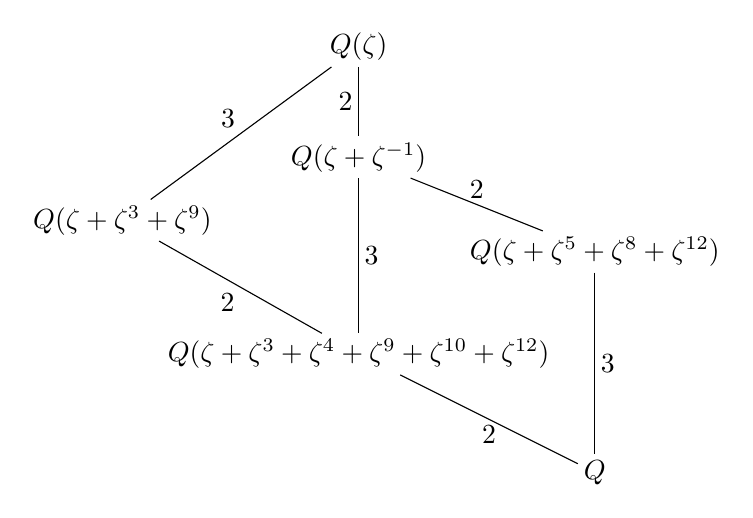
\begin{tikzpicture}[scale=1.0, every node/.style={inner sep=2pt}, baseline=(current bounding box.center)]
\node (top) at (0,3.6) {$\mathbb Q(\zeta)$};
\node (mid) at (0,2.2) {$\mathbb Q(\zeta+\zeta^{-1})$};
\node (left) at (-3.0,1.4) {$\mathbb Q(\zeta+\zeta^3+\zeta^9)$};
\node (right) at (3.0,1.0) {$\mathbb Q(\zeta+\zeta^5+\zeta^8+\zeta^{12})$};
\node (low) at (0,-0.3) {$\mathbb Q(\zeta+\zeta^3+\zeta^4+\zeta^9+\zeta^{10}+\zeta^{12})$};
\node (bot) at (3.0,-1.8) {$\mathbb Q$};
\draw (top)--node[left] {$2$} (mid);
\draw (top)--node[above left] {$3$} (left);
\draw (mid)--node[above] {$2$} (right);
\draw (mid)--node[right] {$3$} (low);
\draw (left)--node[below left] {$2$} (low);
\draw (right)--node[right] {$3$} (bot);
\draw (low)--node[below] {$2$} (bot);
\end{tikzpicture}
\]
式 (10) 中构造的元素以及它们的共轭称为 $\zeta$ 的\emph{周期}，它们在分圆域的算术研究中很有用。对它们的组合性质的研究称为\emph{分圆法}。
\end{enumerate}

设
\[
n=p_1^{a_1}p_2^{a_2}\cdots p_k^{a_k}
\]
是 $n$ 分解为互异素数幂的分解。由于
\[
\zeta_{p_2^{a_2}\cdots p_k^{a_k}}
\]
是一个本原 $p_1^{a_1}$ 次单位根，域 $K_1=\mathbb Q(\zeta_{p_1^{a_1}})$ 是 $\mathbb Q(\zeta_n)$ 的一个子域。类似地，每个域
\[
K_i=\mathbb Q(\zeta_{p_i^{a_i}}),\qquad i=1,2,\ldots,k
\]
都是 $\mathbb Q(\zeta_n)$ 的子域。这些域的复合含有乘积
\[
\zeta_{p_1^{a_1}}\zeta_{p_2^{a_2}}\cdots \zeta_{p_k^{a_k}},
\]
它是一个本原 $n$ 次单位根，因此复合域就是 $\mathbb Q(\zeta_n)$。由于扩张次数 $[K_i:\mathbb Q]$ 等于 $\varphi(p_i^{a_i})$，$i=1,2,\ldots,k$，并且
\[
\varphi(n)=\varphi(p_1^{a_1})\varphi(p_2^{a_2})\cdots\varphi(p_k^{a_k}),
\]
这些域 $K_i$ 的复合的次数正好是各 $K_i$ 的次数的乘积。由命题 21（以及从命题中两个域的情形到这里 $k$ 个域的简单归纳）可知所有这些域的交恰为 $\mathbb Q$。于是推论 22 表明 $\mathbb Q(\zeta_n)$ 的 Galois 群是这些子域 $K_i$ 在 $\mathbb Q$ 上的 Galois 群的直积。我们把这总结为下面的推论。

\noindent\textbf{推论 27.} 设
\[
n=p_1^{a_1}p_2^{a_2}\cdots p_k^{a_k}
\]
是正整数 $n$ 分解为互异素数幂的分解。则分圆域 $\mathbb Q(\zeta_{p_i^{a_i}})$，$i=1,2,\ldots,k$，只在域 $\mathbb Q$ 中相交，并且它们的复合是分圆域 $\mathbb Q(\zeta_n)$。我们有
\[
\operatorname{Gal}(\mathbb Q(\zeta_n)/\mathbb Q)
\cong
\operatorname{Gal}(\mathbb Q(\zeta_{p_1^{a_1}})/\mathbb Q)	imes
\operatorname{Gal}(\mathbb Q(\zeta_{p_2^{a_2}})/\mathbb Q)	imes\cdots\times
\operatorname{Gal}(\mathbb Q(\zeta_{p_k^{a_k}})/\mathbb Q),
\]
而在定理 26 的同构下，这就是中国剩余定理：
\[
(\mathbb Z/n\mathbb Z)^\times
\cong
(\mathbb Z/p_1^{a_1}\mathbb Z)^\times\times
(\mathbb Z/p_2^{a_2}\mathbb Z)^\times\times\cdots\times
(\mathbb Z/p_k^{a_k}\mathbb Z)^\times.
\]

\begin{proof}
唯一尚未证明的断言，是把 Galois 群的这个同构与中国剩余定理在群 $(\mathbb Z/n\mathbb Z)^\times$ 上的陈述相识别；这很简单，留给练习。
\end{proof}

由定理 26，Galois 群 $\operatorname{Gal}(\mathbb Q(\zeta_n)/\mathbb Q)$ 特别是一个 Abel 群。

\noindent\textbf{定义.} 扩张 $K/F$ 称为一个 \emph{Abel 扩张}，如果 $K/F$ 是 Galois 的，并且 $\operatorname{Gal}(K/F)$ 是一个 Abel 群。

由于 Abel 群的所有子群和商群仍然是 Abel 群，由 Galois 理论基本定理可知，一个 $F$ 的 Abel 扩张中任意包含 $F$ 的子域又是 $F$ 的 Abel 扩张。由上一节关于复合扩张的结果，我们还看到 Abel 扩张的复合仍然是 Abel 扩张（因为复合的 Galois 群同构于这些 Galois 群的直积的一个子群，因而是 Abel 群）。

判定哪些群可以作为 $\mathbb Q$ 的 Galois 扩张的 Galois 群，是一个开放问题。利用上面的结果，我们可以看到，每个 Abel 群都作为 $\mathbb Q$ 的某个扩张的 Galois 群出现；事实上，它作为某个分圆域的子域的 Galois 群出现。

令 $n=p_1p_2\cdots p_k$ 是互异素数的乘积。于是由中国剩余定理，
\[
(\mathbb Z/n\mathbb Z)^\times
\cong
(\mathbb Z/p_1\mathbb Z)^\times\times(\mathbb Z/p_2\mathbb Z)^\times\times\cdots\times(\mathbb Z/p_k\mathbb Z)^\times
\cong Z_{p_1-1}\times Z_{p_2-1}\times\cdots\times Z_{p_k-1}. \tag{14.11}
\]

现在设 $G$ 为任意有限 Abel 群。由有限生成 Abel 群基本定理，
\[
G\cong Z_{n_1}\times Z_{n_2}\times\cdots\times Z_{n_k}
\]
对某些整数 $n_1,n_2,\ldots,n_k$ 成立。我们把下列事实看作已知：给定任意整数 $m$，存在无穷多个素数 $p$ 满足 $p\equiv 1\pmod m$（参见第 13.6 节后的练习，它用分圆多项式给出一个证明）。利用这个结果，选择互异素数 $p_1,p_2,\ldots,p_k$，使得
\[
p_1\equiv 1\pmod {n_1},
\]
\[
p_2\equiv 1\pmod {n_2},
\]
\[
\vdots
\]
\[
p_k\equiv 1\pmod {n_k},
\]
并令 $n=p_1p_2\cdots p_k$，如上所述。

由构造可知，$n_i$ 整除 $p_i-1$，$i=1,2,\ldots,k$，所以群 $Z_{p_i-1}$ 有一个阶为 $(p_i-1)/n_i$ 的子群 $H_i$，且它对这个子群的商是阶为 $n_i$ 的循环群。因此，式 (11) 中 $(\mathbb Z/n\mathbb Z)^\times$ 对子群
\[
H_1\times H_2\times\cdots\times H_k
\]
的商同构于群 $G$。

由定理 26 和 Galois 理论基本定理，我们看到 $\mathbb Q(\zeta_{p_1p_2\cdots p_k})$ 有一个在 $\mathbb Q$ 上 Galois 的子域，其 Galois 群为 $G$。我们把这一点总结为下面的推论。

\noindent\textbf{推论 28.} 设 $G$ 为任意有限 Abel 群。则存在某个分圆域的子域 $K$，使得
\[
\operatorname{Gal}(K/\mathbb Q)\cong G.
\]

这个结果有一个逆命题（其证明超出我们的范围），即著名的 Kronecker--Weber 定理：

\noindent\textbf{定理（Kronecker--Weber）.} 设 $K$ 是 $\mathbb Q$ 的一个有限 Abel 扩张。则 $K$ 包含在 $\mathbb Q$ 的某个分圆扩张中。

$\mathbb Q$ 的 Abel 扩张是“最容易的”Galois 扩张（至少就其 Galois 群的结构而言），而上面的结果表明，它们可以由 $\mathbb Q$ 的分圆扩张来分类。若以 $\mathbb Q$ 的其他有限扩张为基域，则描述 Abel 扩张要困难得多。对 $\mathbb Q$ 的任意有限扩张 $F$ 的 Abel 扩张的研究称为类域论。存在一种用与 $F$ 相关的不变量来分类 $F$ 的 Abel 扩张的理论，它极大地推广了 $\mathbb Q$ 上分圆域的结果。然而一般地，Abel 扩张的构造远不如分圆域情形那样显式。一个可以作出这种描述的情形是虚二次域（$D$ 为正时的 $\mathbb Q(\sqrt{-D})$）的 Abel 扩张，在那里 Abel 扩张可以通过添入某些椭圆函数的值来构造（这类似于添入单位根，而单位根是指数函数 $e^x$ 在某些 $x$ 处的值）。研究这类 Abel 扩张的算术以及寻找非 Abel 扩张的类似结果，是当前数学研究中丰富而迷人的领域。

我们以正 $n$ 边形能否用直尺圆规作出的问题结束对分圆域的讨论。

回忆（见第 13.3 节），元素 $\alpha$ 在 $\mathbb Q$ 上可作，当且仅当域 $\mathbb Q(\alpha)$ 包含在一个域 $K$ 中，而 $K$ 由一串二次扩张得到：
\[
\mathbb Q=K_0\subset K_1\subset\cdots\subset K_i\subset K_{i+1}\subset\cdots\subset K_m=K, \tag{14.12}
\]
其中
\[
[K_{i+1}:K_i]=2,
\qquad i=0,1,\ldots,m-1.
\]

在 $\mathbb R^2$ 中作正 $n$ 边形显然等价于作出 $n$ 次单位根，因为 $n$ 次单位根就是复平面 $\mathbb C$ 中单位圆上以点 $1$ 为一个顶点的正 $n$ 边形的顶点。

作出 $\zeta_n$ 等价于作出 $\zeta_n$ 在 $\mathbb R^2$ 中的第一坐标 $x$，即 $\zeta_n$ 的实部。由于 $\zeta_n$ 的复共轭正是 $\zeta_n^{-1}$，$\zeta_n$ 的实部为
\[
x=\frac12(\zeta_n+\zeta_n^{-1}).
\]
注意 $\zeta_n$ 在 $\mathbb Q(x)$ 上满足二次方程
\[
\zeta_n^2-2x\zeta_n+1=0.
\]
由于 $\mathbb Q(x)$ 只含有实数，故 $[\mathbb Q(\zeta_n):\mathbb Q(x)]=2$，从而 $\mathbb Q(x)$ 是 $\mathbb Q$ 的一个次数为 $\varphi(n)/2$ 的扩张。

于是，如果正 $n$ 边形可以由直尺圆规作出，那么 $\varphi(n)$ 必须是 $2$ 的幂。反过来，如果 $\varphi(n)=2^m$ 是 $2$ 的幂，则 Galois 群 $\operatorname{Gal}(\mathbb Q(\zeta_n)/\mathbb Q)$ 是一个阶为 $2$ 的幂的 Abel 群，所以 $\operatorname{Gal}(\mathbb Q(x)/\mathbb Q)$ 也有同样性质。由 Abel 群基本定理很容易看出，任意阶为 $2^m$ 的 Abel 群 $G$ 有一列子群
\[
G=G_m>G_{m-1}>\cdots>G_{i+1}>G_i>\cdots>G_0=1
\]
且
\[
[G_{i+1}:G_i]=2,
\qquad i=0,1,2,\ldots,m-1.
\]
把这应用到群 $G=\operatorname{Gal}(\mathbb Q(x)/\mathbb Q)$，并取子群 $G_i$，$i=0,1,\ldots,m-1$ 的固定域，由 Galois 理论基本定理得到如式 (12) 的一列二次扩张。

我们得出结论：正 $n$ 边形可以用直尺圆规作出，当且仅当 $\varphi(n)$ 是 $2$ 的幂。把 $n$ 分解成素数幂以计算 $\varphi(n)$，我们看到这意味着
\[
n=2^k p_1\cdots p_r
\]
是 $2$ 的一个幂与互异奇素数 $p_i$ 的乘积，其中每个 $p_i-1$ 都是 $2$ 的幂。初等练习可知，若素数 $p$ 满足 $p-1$ 是 $2$ 的幂，则 $p$ 必须形如
\[
p=2^{2^s}+1
\]
对某个整数 $s$ 成立。这样的素数称为 Fermat 素数。最初几个是
\[
3=2^1+1,
\]
\[
5=2^2+1,
\]
\[
17=2^4+1,
\]
\[
257=2^8+1,
\]
\[
65537=2^{16}+1.
\]
（但 $2^{32}+1$ 不是素数，因为它被 $641$ 整除。）目前尚不知道是否有无穷多个 Fermat 素数。我们把这总结为下面的命题。

\noindent\textbf{命题 29.} 正 $n$ 边形可以用直尺圆规作出，当且仅当
\[
n=2^k p_1\cdots p_r
\]
是 $2$ 的一个幂与互异 Fermat 素数的乘积。

上面的证明实际上给出了一种通过一串平方根来作正 $n$ 边形的程序。例如，正 $17$ 边形的作图（Gauss 于 1796 年、19 岁时解决）需要构造 $\mathbb Q(\zeta_{17})$ 中次数为 $2,4,8,16$ 的子域。这些子域可以通过形成 $\zeta_{17}$ 的周期来构造，如同上面 $13$ 次单位根的例子一样。在这种情形下，$\mathbb Q(\zeta_{17})$ 由一列二次扩张得到这一事实，反映为周期可以逐次“对半分”（也就是说，如果 $H_1<H_2$ 是子群且 $[H_2:H_1]=2$，那么 $H_1$ 的周期满足一个二次方程，其系数涉及 $H_2$ 的周期）。例如，Galois 群中指数为 $2$ 的子群（由 $\sigma^2$ 生成）的周期为（$\zeta=\zeta_{17}$）
\[
\eta_1=\zeta+\zeta^2+\zeta^4+\zeta^8+\zeta^9+\zeta^{13}+\zeta^{15}+\zeta^{16}
\]
和
\[
\eta_2=\zeta^3+\zeta^5+\zeta^6+\zeta^7+\zeta^{10}+\zeta^{11}+\zeta^{12}+\zeta^{14},
\]
它们把整个 Galois 群的周期“对半分”，并满足
\[
\eta_1+\eta_2=-1
\]
（由 $\zeta_{17}$ 满足的极小多项式得到）以及
\[
\eta_1\eta_2=-4
\]
（这需要计算；由 Galois 理论可知它必为有理数，因为这个乘积被 Galois 群的所有元素固定）。因此这两个周期是二次方程
\[
x^2+x-4=0
\]
的根，我们可以显式求解它。类似地，指数为 $4$ 的子群（由 $\sigma^4$ 生成）的周期自然把这些周期再对半分，因此在这些周期上是二次的，依此类推。这样可以用迭代平方根显式确定 $\zeta_{17}$。例如，可以求得
\[
8(\zeta+\zeta^{-1})=16\cos\frac{2\pi}{17}
\]
（这足以作出正 $17$ 边形）显式地等于
\[
-1+\sqrt{17}+\sqrt{2(17-\sqrt{17})}
+2\sqrt{17+3\sqrt{17}-\sqrt{2(17-\sqrt{17})}-2\sqrt{2(17+\sqrt{17})}}.
\]

一个相对简单的正 $17$ 边形作图（由 J. H. Conway 向我们展示）在练习中给出。

虽然我们已经看到，一般不能仅用连续开平方来求出 $\zeta_n$，但按定义可以通过连续开高次根得到 $\zeta_n$（即取 $1$ 的一个 $n$ 次根）。对于一般 $n$ 次方程的解，这种情形不再成立；一般不能用根式确定其解，我们将在下面几节中看到这一点。

\subsection*{练习}
\begin{enumerate}[label=\arabic*.]
\item 求正文中给出的 $\mathbb Q(\zeta_{13})$ 的各子域的本原生成元所满足的极小多项式。

\item 求由 $\zeta_8$ 的周期生成的 $\mathbb Q(\zeta_8)$ 的子域，并且特别证明并非每个子域都有这样的周期作为本原元。

\item 求 $5$ 次单位根 $\zeta_5$ 的周期 $\alpha=\zeta_5+\zeta_5^{-1}$ 所满足的二次方程。求 $\zeta_5$ 在 $\mathbb Q(\alpha)$ 上所满足的二次方程，并利用它显式求出 $5$ 次单位根。

\item 设 $\sigma_a\in\operatorname{Gal}(\mathbb Q(\zeta_n)/\mathbb Q)$ 表示 $n$ 次单位根分圆域中的自同构，它把 $\zeta_n$ 映到 $\zeta_n^a$，其中 $a$ 与 $n$ 互素且 $\zeta_n$ 是一个本原 $n$ 次单位根。证明对每个 $n$ 次单位根 $\zeta$，都有
\[
\sigma_a(\zeta)=\zeta^a.
\]

\item 设 $p$ 为素数，令 $\epsilon_1,\epsilon_2,\ldots,\epsilon_{p-1}$ 表示本原 $p$ 次单位根。置
\[
P_n=\epsilon_1^n+\epsilon_2^n+\cdots+\epsilon_{p-1}^n,
\]
即所有 $\epsilon_i$ 的 $n$ 次幂之和。证明若 $p$ 不整除 $n$，则 $P_n=-1$；若 $p$ 整除 $n$，则 $P_n=p-1$。〔一种方法：由 $\Phi_p(x)$ 得 $P_1=-1$；证明若 $p$ 不整除 $n$，则 $P_n$ 是 $P_1$ 的一个 Galois 共轭，因此也等于 $-1$。〕

\item 令 $\zeta_n$ 表示一个本原 $n$ 次单位根，令 $K=\mathbb Q(\zeta_n)$ 为相应分圆域。令 $a$ 表示 $\zeta_n$ 从 $K$ 到 $\mathbb Q$ 的迹（参见第 14.2 节练习 18）。证明：若 $n=1$，则 $a=1$；若 $n$ 被某个素数的平方整除，则 $a=0$；若 $n$ 是 $r$ 个互异素数的乘积，则 $a=(-1)^r$。

\item 证明复共轭限制到 $n$ 次单位根分圆域 $\mathbb Q(\zeta_n)$ 上就是自同构 $\sigma_{-1}\in\operatorname{Gal}(\mathbb Q(\zeta_n)/\mathbb Q)$。证明
\[
K^+=\mathbb Q(\zeta_n+\zeta_n^{-1})
\]
是 $K=\mathbb Q(\zeta_n)$ 中实元素组成的子域，称为 $K$ 的极大实子域。

\item 令 $K_n=\mathbb Q(\zeta_{2^{n+2}})$ 为 $2^{n+2}$ 次单位根的分圆域，$n\geq 0$。置
\[
\alpha_n=\zeta_{2^{n+2}}+\zeta_{2^{n+2}}^{-1},
\qquad
K_n^+=\mathbb Q(\alpha_n),
\]
即 $K_n$ 的极大实子域。
\begin{enumerate}[label=(\alph*)]
\item 证明对所有 $n\geq 0$，
\[
[K_n:\mathbb Q]=2^{n+1},\qquad [K_n:K_n^+]=2,
\]
\[
[K_n^+:\mathbb Q]=2^n,
\qquad [K_{n+1}^+:K_n^+]=2.
\]

\item 用 $\alpha_n$ 表示 $\zeta_{2^{n+2}}$ 在 $K_n^+$ 上所满足的二次方程。

\item 证明对 $n\geq 0$，
\[
\alpha_{n+1}^2=2+\alpha_n,
\]
并由此证明
\[
\alpha_n=\sqrt{2+\sqrt{2+\cdots+\sqrt2}}
\]
（共 $n$ 次），从而给出可作的 $2^{n+2}$ 次单位根的一个显式公式。
\end{enumerate}

\item 沿用前一题的记号。
\begin{enumerate}[label=(\alph*)]
\item 证明 $K_n^+$ 是 $\mathbb Q$ 的次数为 $2^n$ 的循环扩张。〔使用 Abel 群的一个显式同构
\[
(\mathbb Z/2^{n+2}\mathbb Z)^\times\cong \mathbb Z/2\mathbb Z\times\mathbb Z/2^n\mathbb Z
\]
（即 $(\mathbb Z/2^{n+2}\mathbb Z)^\times$ 同构于一个阶为 $2$ 的循环群与一个阶为 $2^n$ 的循环群的直积；参见第 2.3 节练习 22 和 23）。〕

\item 证明 $K_n$ 是 $K_{n-1}^+$ 的二二次扩张，并且三个中间域中的两个是 $K_n^+$ 和 $K_{n-1}$。证明 $K_{n-1}^+$ 与 $K_n$ 之间剩下的那个中间域是 $\mathbb Q$ 的次数为 $2^n$ 的循环扩张。
\end{enumerate}

\item 证明 $\mathbb Q(\sqrt[3]{2})$ 不是 $\mathbb Q$ 上任一分圆域的子域。

\item 证明本原 $n$ 次单位根构成 $n$ 次单位根分圆域在 $\mathbb Q$ 上的一组基，当且仅当 $n$ 是无平方因子的（即 $n$ 不被任一素数的平方整除）。

\item 设 $\sigma_p$ 表示有限域 $\mathbb F_q$（其中 $q=p^n$）的 Frobenius 自同构
\[
x\longmapsto x^p.
\]
把 $\mathbb F_q$ 看作 $\mathbb F_p$ 上的 $n$ 维向量空间 $V$，于是可以把 $\sigma_p$ 看作 $V$ 到自身的线性变换。求 $\sigma_p$ 的特征多项式，并证明：线性变换 $\sigma_p$ 在 $\mathbb F_p$ 上可对角化，当且仅当 $n$ 整除 $p-1$；它在 $\mathbb F_p$ 的代数闭包上可对角化，当且仅当 $(n,p)=1$。

\item 设
\[
n=p_1^{a_1}p_2^{a_2}\cdots p_k^{a_k}
\]
为 $n$ 的素因子分解，令 $\zeta_n$ 是一个本原 $n$ 次单位根。对每个 $i=1,2,\ldots,k$，定义 $d_i$ 由
\[
n=p_i^{a_i}d_i
\]
给出，并令
\[
\zeta_{p_i^{a_i}}=\zeta_n^{d_i},
\]
于是 $\zeta_{p_i^{a_i}}$ 是一个特定的本原 $p_i^{a_i}$ 次单位根。令 $\sigma_a\in\operatorname{Gal}(\mathbb Q(\zeta_n)/\mathbb Q)$ 为把 $\zeta_n$ 映到 $\zeta_n^a$ 的自同构，其中 $a$ 与 $n$ 互素。
\begin{enumerate}[label=(\alph*)]
\item 证明对 $i=1,2,\ldots,k$，$\sigma_a$ 把 $\zeta_{p_i^{a_i}}$ 映到 $\zeta_{p_i^{a_i}}^a$，并给出 $\mathbb Q(\zeta_{p_i^{a_i}})/\mathbb Q$ 的一个只依赖于 $a\pmod {p_i^{a_i}}$ 的自同构，我们可将它记为 $\sigma_{a\,({\rm mod}\,p_i^{a_i})}$。

\item 证明映射
\[
\sigma_a\longmapsto
\bigl(\sigma_{a\,({\rm mod}\,p_1^{a_1})},\ldots,
\sigma_{a\,({\rm mod}\,p_k^{a_k})}\bigr)
\]
就是推论 27 中对应于 $(\mathbb Z/n\mathbb Z)^\times$ 的中国剩余定理的同构。
\end{enumerate}

以下练习 14 到 18 确定与一个本原 $17$ 次单位根相关的周期，并给出练习 17 中指出的正 $17$ 边形的简单几何作图的证明。令
\[
\zeta=\zeta_{17}=\cos\frac{2\pi}{17}+i\sin\frac{2\pi}{17}
\]
为 $\mathbb C$ 中一个固定的本原 $17$ 次单位根。

\item 定义 $\zeta$ 的周期如下：
\[
\eta_1=\zeta+\zeta^2+\zeta^4+\zeta^8+\zeta^9+\zeta^{13}+\zeta^{15}+\zeta^{16},
\qquad
\eta_3'=\zeta^6+\zeta^7+\zeta^{10}+\zeta^{11},
\]
\[
\eta_2=\zeta^3+\zeta^5+\zeta^6+\zeta^7+\zeta^{10}+\zeta^{11}+\zeta^{12}+\zeta^{14},
\qquad
\eta_4'=\zeta^3+\zeta^5+\zeta^{12}+\zeta^{14},
\]
\[
\eta_1'=\zeta+\zeta^4+\zeta^{13}+\zeta^{16},
\qquad
\eta_1''=\zeta+\zeta^{16},
\]
\[
\eta_2'=\zeta^2+\zeta^8+\zeta^9+\zeta^{15},
\qquad
\eta_2''=\zeta^4+\zeta^{13}.
\]
\begin{enumerate}[label=(\alph*)]
\item 证明所有这些周期都是实数，并且
\[
\eta_1''=2\cos\frac{2\pi}{17}.
\]
证明作为实数，这些周期近似为
\[
\eta_1\approx 1.562,
\quad
\eta_1'\approx 2.049,
\quad
\eta_3'\approx -2.906,
\quad
\eta_1''\approx 1.865,
\]
\[
\eta_2\approx -2.562,
\quad
\eta_2'\approx -0.488,
\quad
\eta_4'\approx 0.344,
\quad
\eta_2''\approx 0.185.
\]

\item 证明 $\eta_1$ 和 $\eta_2$ 是方程
\[
x^2+x-4=0
\]
的根。

\item 证明 $\eta_1'$ 和 $\eta_2'$ 是方程
\[
x^2-\eta_1x-1=0
\]
的根，并且 $\eta_3'$ 和 $\eta_4'$ 是方程
\[
x^2-\eta_2x-1=0
\]
的根。

\item 证明 $\eta_1''$ 和 $\eta_2''$ 是方程
\[
x^2-\eta_1'x+\eta_2'=0
\]
的根。
\end{enumerate}

\item 证明若 $\tan 2\theta=a$，其中 $0<2\theta<\pi/2$，则 $\tan\theta$ 满足方程
\[
x^2-\frac{2}{a}x-1=0.
\]

\item 令 $C$ 为 $\mathbb R^2$ 中以点 $(h,k)$ 和 $(0,1)$ 为直径的圆。证明这个圆与 $x$ 轴相交，当且仅当 $h^2-4k\geq 0$；并且在这种情形中，两个截距是方程
\[
x^2-hx+k=0
\]
的根。

\item （正 $17$ 边形的作图）画一个以原点 $(0,0)$ 为圆心、半径为 $2$ 的圆。
\begin{enumerate}[label=(\alph*)]
\item 连接点 $(4,0)$ 与点 $(0,1)$，并作直线 $\ell_1$，它平分这条直线与 $y$ 轴之间的角。作直线 $\ell_2$ 垂直于图 2 中的 $\ell_1$。

\begin{center}
\begin{tikzpicture}[scale=0.75, every node/.style={inner sep=2pt}]
\draw[->] (-3.2,0)--(4.7,0) node[right] {$x$};
\draw[->] (0,-2.4)--(0,2.7) node[above] {$y$};
\draw (0,0) circle (2);
\fill (4,0) circle (1.5pt) node[below] {$(4,0)$};
\fill (0,1) circle (1.5pt) node[left] {$(0,1)$};
\draw (4,0)--(0,1);
\draw[dashed] (0,-2.2)--(0,2.5);
\draw[thick] (-2.6,-1.5)--(2.1,1.2) node[right] {$\ell_1$};
\draw[thick] (-1.0,2.3)--(1.4,-1.9) node[right] {$\ell_2$};
\node at (3.8,-1.5) {图 2};
\end{tikzpicture}
\end{center}

\item 以 $\ell_1$ 与 $x$ 轴的交点为圆心，并取到 $(0,1)$ 的距离为半径作圆 $C_1$，令 $A=(s,0)$ 为 $C_1$ 与 $x$ 轴右侧的交点。类似地，令 $B=(t,0)$ 表示 $x$ 轴与圆 $C_2$ 的右侧交点，其中 $C_2$ 的圆心是 $\ell_2$ 与 $x$ 轴的交点，半径等于到 $(0,1)$ 的距离，如图 3 所示。

\begin{center}
\begin{tikzpicture}[scale=0.75, every node/.style={inner sep=2pt}]
\draw[->] (-3.2,0)--(4.7,0) node[right] {$x$};
\draw[->] (0,-2.4)--(0,2.7) node[above] {$y$};
\draw (0,0) circle (2);
\fill (0,1) circle (1.5pt) node[left] {$(0,1)$};
\coordinate (O1) at (0.8,0);
\coordinate (O2) at (-1.3,0);
\draw[thick] (O1) circle (1.28);
\draw[thick] (O2) circle (1.64);
\draw[dashed] (O1)--(0,1);
\draw[dashed] (O2)--(0,1);
\fill (2.08,0) circle (1.5pt) node[below] {$A=(s,0)$};
\fill (0.34,0) circle (1.5pt) node[below] {$B=(t,0)$};
\node at (1.4,1.4) {$C_1$};
\node at (-2.4,1.2) {$C_2$};
\node at (3.8,-1.5) {图 3};
\end{tikzpicture}
\end{center}

\item 在点 $A$ 处作 $x$ 轴的垂线，并把从 $(0,0)$ 到 $B$ 的距离 $t$ 标出，从而作出点 $(s,t)$。作以 $(s,t)$ 和 $(0,1)$ 为直径的圆，令 $P$ 为这个圆与 $x$ 轴的右侧交点。过 $P$ 作 $x$ 轴的垂线，它与半径为 $2$ 的圆相交于正 $17$ 边形的第二个顶点，而第一个顶点取为 $(2,0)$；于是如图 4 所示，用直尺圆规作出了正 $17$ 边形。

\begin{center}
\begin{tikzpicture}[scale=0.75, every node/.style={inner sep=2pt}]
\draw[->] (-3.2,0)--(4.7,0) node[right] {$x$};
\draw[->] (0,-2.4)--(0,2.7) node[above] {$y$};
\draw (0,0) circle (2);
\fill (2,0) circle (1.5pt) node[below right] {$(2,0)$};
\fill (0,1) circle (1.5pt) node[left] {$(0,1)$};
\fill (1.6,0) circle (1.5pt) node[below] {$P$};
\draw[dashed] (1.6,-0.1)--(1.6,2.1);
\fill (1.6,1.2) circle (1.5pt) node[right] {第二顶点};
\fill (1.1,0.6) circle (1.2pt) node[right] {$(s,t)$};
\draw[thick] (0.55,0.8) circle (0.78);
\draw[dashed] (0,1)--(1.1,0.6);
\draw[dashed] (1.1,0.6)--(1.6,0);
\node at (3.8,-1.5) {图 4};
\end{tikzpicture}
\end{center}
\end{enumerate}

\item 沿用前一练习的记号。
\begin{enumerate}[label=(\alph*)]
\item 证明 $\ell_1$ 与 $x$ 轴交于点 $(\eta_1/2,0)$，并且 $\ell_2$ 与 $x$ 轴交于点 $(\eta_2/2,0)$。

\item 证明 $C_1$ 是以点 $(\eta_1,-1)$ 和 $(0,1)$ 为直径的圆。证明 $s=\eta_1'$。类似地，证明 $C_2$ 是以点 $(\eta_2,-1)$ 和 $(0,1)$ 为直径的圆，并且 $t=\eta_4'$。

\item 证明 $P$ 的坐标为 $(\eta_1'',0)$，从而前一题中的作图确实用直尺圆规作出了正 $17$ 边形。
\end{enumerate}
\end{enumerate}

\section{多项式的 Galois 群}

回忆：可分多项式 $f(x)\in F[x]$ 的 Galois 群，定义为 $f(x)$ 的分裂域在 $F$ 上的 Galois 群。

若 $K$ 是 $F$ 的 Galois 扩张，则 $K$ 是 $F$ 上某个可分多项式 $f(x)$ 的分裂域。任意自同构 $\sigma\in \operatorname{Gal}(K/F)$ 都把 $f(x)$ 的一个不可约因子的一个根映到同一不可约因子的另一个根，并且 $\sigma$ 由它在这些根上的作用唯一确定（因为这些根在 $F$ 上生成 $K$）。如果固定 $f(x)$ 的根 $\alpha_1,\ldots,\alpha_n$ 的一个标号，则每个 $\sigma\in\operatorname{Gal}(K/F)$ 都定义了 $\alpha_1,\\ldots,\alpha_n$ 的一个唯一置换，因而定义了下标集合 $\{1,2,\ldots,n\}$ 的一个唯一置换（这个置换依赖于所固定的根的标号）。于是得到一个单射
\[
\operatorname{Gal}(K/F)\hookrightarrow S_n
\]
把 Galois 群嵌入 $n$ 个字母上的对称群；这显然是一个同态（两个群的运算都是复合）。因此我们可以把 Galois 群看成对称群的子群。由于由基本定理知分裂域的次数等于 Galois 群的阶，这也从群论方面解释了为什么 $F$ 上一个 $n$ 次多项式的分裂域次数至多为 $n!$（命题 13.26）。

一般地，如果 $f(x)$ 分解为不可约因子的乘积
\[
f(x)=f_1(x)\cdots f_k(x),
\]
其中 $\deg f_i=n_i$，$i=1,2,\ldots,k$，则 Galois 群只在每个不可约因子的根之间作置换，因此
\[
\operatorname{Gal}(K/F)\leq S_{n_1}\times\cdots\times S_{n_k}.
\]
如果 $f(x)$ 是不可约的，那么给定 $f(x)$ 的任意两个根，存在 $f(x)$ 的 Galois 群 $G$ 中的一个自同构把第一个根映到第二个根（这来自扩张定理 13.27）。这样的群称为在根上传递；也就是说，可以通过作用某个 $G$ 的元素从任意给定的根到达任意另一个根。Galois 群必须在根的块（即不可约因子的根）上传递这一事实，常常有助于减少 $G$ 的可能结构（参见下面关于四次多项式的 Galois 群的讨论）。

\paragraph{例}
\begin{enumerate}[label=(\arabic*)]
\item 考虑双二次扩张 $\mathbb Q(\sqrt2,\sqrt3)$ 在 $\mathbb Q$ 上的扩张，它是 $(x^2-2)(x^2-3)$ 的分裂域。把根标号为
\[
\alpha_1=\sqrt2,\qquad \alpha_2=-\sqrt2,\qquad \alpha_3=\sqrt3,
\qquad \alpha_4=-\sqrt3.
\]
Galois 群的元素为 $\{1,\sigma,\tau,\sigma\tau\}$，其中 $\sigma$ 把 $\sqrt2$ 映到 $-\sqrt2$ 并固定 $\sqrt3$，而 $\tau$ 固定 $\sqrt2$ 并把 $\sqrt3$ 映到 $-\sqrt3$。作为在这些根上的置换，$\sigma$ 交换前两个根并固定后两个根，而 $\tau$ 固定前两个根并交换后两个根；也就是说，作为 $S_4$ 的元素，
\[
\sigma=(12),\qquad \tau=(34),\qquad \sigma\tau=(12)(34).
\]
因此
\[
\operatorname{Gal}(\mathbb Q(\sqrt2,\sqrt3)/\mathbb Q)
\cong \{1,(12),(34),(12)(34)\}\leq S_4,
\]
这把该 Galois 群识别为 $S_4$ 中的 Klein 四元子群。注意，如果改变上面根的标号，就会得到 Galois 群作为 $S_4$ 子群的另一个（同构的）表示；例如，若交换第二个根与第三个根，则得到子群 $\{1,(13),(24),(13)(24)\}$。

\item $x^3-2$ 的 Galois 群作用在三个根
\[
\sqrt[3]{2},\qquad \rho\sqrt[3]{2},\qquad \rho^2\sqrt[3]{2}
\]
上，其中 $\rho$ 是本原三次单位根。按这个顺序排列，先前定义的生成元 $\sigma$ 与 $\tau$ 给出置换
\[
\sigma=(123),\qquad \tau=(23),
\]
于是
\[
\{1,\sigma,\sigma^2,\tau,\sigma\tau,\sigma\tau^2\}
=\{1,(123),(132),(23),(13),(12)\}=S_3.
\]
在这个情形中，Galois 群是三个字母上的整个对称群。
\end{enumerate}

回忆，每个有限群都同构于某个对称群 $S_n$ 的子群。判断每个有限群是否都能作为 $\mathbb Q$ 上某个多项式的 Galois 群，是一个开放问题。我们在上一节已经看到，每个有限 Abel 群都是 $\mathbb Q$ 上某个 Galois 群（来自某个分圆域的子域）。下面我们将显式确定低次数（$\leq 4$）多项式的 Galois 群；这特别会表明 $S_4$ 的每个子群都作为 Galois 群出现。

我们首先引入若干定义，并说明 $n$ 次“一般”多项式的 Galois 群是 $S_n$（因此上面第二个例子应视为“典型”的）。

\noindent\textbf{定义.} 令 $x_1,x_2,\ldots,x_n$ 为不定元。\emph{基本对称函数} $s_1,s_2,\ldots,s_n$ 定义为
\[
\begin{aligned}
s_1&=x_1+x_2+\cdots+x_n,\\
s_2&=x_1x_2+x_1x_3+\cdots+x_2x_3+x_2x_4+\cdots+x_{n-1}x_n,\\
&\ \vdots\\
s_n&=x_1x_2\cdots x_n;
\end{aligned}
\]
也就是说，$x_1,x_2,\ldots,x_n$ 的第 $i$ 个对称函数 $s_i$ 是所有一次取 $i$ 个 $x_j$ 的乘积之和。

\noindent\textbf{定义.} \emph{$n$ 次一般多项式}是多项式
\[
(x-x_1)(x-x_2)\cdots(x-x_n),
\]
其根是不定元 $x_1,x_2,\ldots,x_n$。

容易用归纳看出，$n$ 次一般多项式的系数由根的基本对称函数给出：
\begin{equation}
(x-x_1)(x-x_2)\cdots(x-x_n)=x^n-s_1x^{n-1}+s_2x^{n-2}+\cdots+(-1)^n s_n.\tag{14.13}
\end{equation}

对任意域 $F$，扩张 $F(x_1,x_2,\ldots,x_n)$ 是 $F(s_1,s_2,\ldots,s_n)$ 上的 Galois 扩张，因为它是 $n$ 次一般多项式的分裂域。

若 $\sigma\in S_n$ 是 $\{1,2,\ldots,n\}$ 的任意置换，则 $\sigma$ 通过置换变量 $x_1,x_2,\ldots,x_n$ 的下标作用在 $F(x_1,x_2,\ldots,x_n)$ 中的有理函数上。显然这给出 $F(x_1,x_2,\ldots,x_n)$ 的一个自同构。把 $\sigma\in S_n$ 与这个自同构相识别，便把 $S_n$ 识别为 $\operatorname{Aut}(F(x_1,x_2,\ldots,x_n))$ 的一个子群。

基本对称函数 $s_1,s_2,\ldots,s_n$ 在下标的任意置换下都保持不变（这就是称它们为对称的原因），这说明子域 $F(s_1,s_2,\ldots,s_n)$ 包含在 $S_n$ 的固定域中。由 Galois 理论基本定理，$S_n$ 的固定域在 $F(x_1,x_2,\ldots,x_n)$ 中的指数恰为 $n!$。另一方面，因为 $F(x_1,x_2,\ldots,x_n)$ 是式 (14.13) 的 $n$ 次多项式在 $F(s_1,s_2,\ldots,s_n)$ 上的分裂域，我们有
\begin{equation}
[F(x_1,x_2,\ldots,x_n):F(s_1,s_2,\ldots,s_n)]\leq n!.\tag{14.14}
\end{equation}
于是实际上必有等号，并且 $F(s_1,s_2,\ldots,s_n)$ 正是 $S_n$ 的固定域。这证明了如下结果。

\noindent\textbf{命题 30.} 对称群 $S_n$ 作用在 $n$ 个变量的有理函数域 $F(x_1,x_2,\ldots,x_n)$ 上时，它的固定域是基本对称函数生成的有理函数域
\[
F(s_1,s_2,\ldots,s_n).
\]

\noindent\textbf{定义.} 若有理函数 $f(x_1,x_2,\ldots,x_n)$ 在变量 $x_1,x_2,\ldots,x_n$ 的任意置换下都不变，则称它是\emph{对称的}。

\noindent\textbf{推论 31（对称函数基本定理）.} 变量 $x_1,x_2,\ldots,x_n$ 中的任意对称函数都是基本对称函数 $s_1,s_2,\ldots,s_n$ 的有理函数。

\begin{proof}
对称函数属于上面 $S_n$ 的固定域，因而是 $s_1,\ldots,s_n$ 的有理函数。
\end{proof}

这个推论解释了为什么这些函数称为基本对称函数。

\paragraph{注记}
如果 $f(x_1,\ldots,x_n)$ 是 $x_1,x_2,\ldots,x_n$ 中的一个对称多项式，那么可以看出 $f$ 实际上是 $s_1,s_2,\ldots,s_n$ 的一个多项式；这加强了推论的结论。事实上，如果 $R$ 是任意含 $1$ 的交换环，则系数属于 $R$ 的对称多项式，都是系数属于 $R$ 的基本对称函数多项式。练习中给出的把对称多项式写成基本对称函数多项式的算法，隐含着这个事实的证明。

\paragraph{例}
\begin{enumerate}[label=(\arabic*)]
\item 表达式 $(x_1-x_2)^2$ 关于 $x_1,x_2$ 对称。我们有
\[
(x_1-x_2)^2=(x_1+x_2)^2-4x_1x_2=s_1^2-4s_2,
\]
这是基本对称函数的多项式。

\item 多项式 $x_1^2+x_2^2+x_3^2$ 关于 $x_1,x_2,x_3$ 对称，在此情形中
\[
x_1^2+x_2^2+x_3^2=(x_1+x_2+x_3)^2-2(x_1x_2+x_1x_3+x_2x_3)=s_1^2-2s_2.
\]

\item 多项式 $x_1^2x_2^2+x_1^2x_3^2+x_2^2x_3^2$ 是对称的。由于
\[
\begin{aligned}
(x_1x_2+x_1x_3+x_2x_3)^2
&=x_1^2x_2^2+x_1^2x_3^2+x_2^2x_3^2 \\
&\quad+2(x_1^2x_2x_3+x_2^2x_1x_3+x_3^2x_1x_2)\\
&=x_1^2x_2^2+x_1^2x_3^2+x_2^2x_3^2+2x_1x_2x_3(x_1+x_2+x_3),
\end{aligned}
\]
所以
\[
x_1^2x_2^2+x_1^2x_3^2+x_2^2x_3^2=s_2^2-2s_1s_3.
\]
\end{enumerate}

现在假设我们从一般多项式
\[
x^n-s_1x^{n-1}+s_2x^{n-2}+\cdots+(-1)^n s_n
\]
出发，把它看作域 $F(s_1,s_2,\ldots,s_n)$ 上的多项式，其中 $s_i$，$i=1,2,\ldots,n$，被看作不定元。如果定义这个多项式的根为 $x_1,x_2,\ldots,x_n$，则 $s_i$ 恰好是根 $x_1,\ldots,x_n$ 的基本对称函数。此外，这些根本身也是不定元，也就是说它们之间在 $F$ 上没有多项式关系。事实上，若 $p(t_1,\ldots,t_n)$ 是 $n$ 个变量中系数在 $F$ 中的一个非零多项式，并且 $p(x_1,\ldots,x_n)=0$，则取 $S_n$ 中所有置换 $\sigma$ 的乘积
\[
\prod_{\sigma\in S_n}p(t_{\sigma(1)},\ldots,t_{\sigma(n)}),
\]
得到一个非零对称多项式，它在 $(x_1,
\ldots,x_n)$ 处为 $0$。这会给出 $s_1,\ldots,s_n$ 之间在 $F$ 上的非零多项式关系，矛盾。反过来，如果一个多项式 $f(x)$ 的根在 $F$ 上是独立的不定元，则 $f(x)$ 的系数也是如此；参见第 9 节开头。因此，用“不定根”定义一般多项式，与用“不定系数”定义一般多项式是等价的。从这个观点出发，上述结果可以表述为：

\noindent\textbf{定理 32.} 一般多项式
\[
x^n-s_1x^{n-1}+s_2x^{n-2}+\cdots+(-1)^n s_n
\]
在域 $F(s_1,s_2,\ldots,s_n)$ 上可分，并且其 Galois 群为 $S_n$。

这个结果说，如果 $n$ 次多项式的系数之间没有关系（这就是上面说 $s_i$ 是不定元的含义），那么这个多项式在由其系数生成的域上的 Galois 群就是完整的对称群 $S_n$。粗略地说，这意味着“泛型”的 $n$ 次多项式会有 $S_n$ 作为 Galois 群。不过要注意，在有限域上每个多项式的 Galois 群都是循环群（有限域的所有扩张都是循环的），所以这种意义下的“泛型”多项式并不存在。在 $\mathbb Q$ 上，可以把“泛型”多项式的概念精确化；于是大多数多项式确有完整的对称群作为 Galois 群。

当 $n\geq 5$ 时，$S_n$ 只有一个非平凡正规子群，即指数为 $2$ 的子群 $A_n$。因此一般地，$F(x_1,x_2,\ldots,x_n)$ 中含有 $F(s_1,s_2,\ldots,s_n)$ 的正规子域只有一个，并且它是 $2$ 次扩张。

\noindent\textbf{定义.} 定义 $x_1,x_2,\ldots,x_n$ 的\emph{判别式} $D$ 为
\[
D=\prod_{i<j}(x_i-x_j)^2.
\]
多项式的判别式定义为其根的判别式。

判别式 $D$ 是 $x_1,
\ldots,x_n$ 中的对称函数，因而属于 $K=F(s_1,s_2,\ldots,s_n)$。

当我们最初定义交错群 $A_n$ 时已经看到，一个置换 $\sigma\in S_n$ 属于子群 $A_n$ 当且仅当它固定乘积
\[
\sqrt D=\prod_{i<j}(x_i-x_j)\in \mathbb Z[x_1,x_2,\ldots,x_n].
\]
因此（由基本定理），若 $F$ 的特征不为 $2$，则 $\sqrt D$ 生成 $A_n$ 的固定域，并且生成 $K$ 的一个二次扩张。这证明了如下命题。

\noindent\textbf{命题 33.} 若 $\operatorname{ch}(F)\neq 2$，则置换 $\sigma\in S_n$ 属于 $A_n$ 当且仅当它固定判别式 $D$ 的平方根。

现在我们考虑域 $F$ 上小次数（$\leq 4$）的可分多项式的 Galois 群，并假设 $F$ 的特征不是 $2$ 或 $3$。注意，在 $\mathbb Q$ 上或在有限域上（更一般地，在任意完美域上），任意多项式 $f(x)$ 的分裂域与把 $f(x)$ 的不可约因子各取一次后的乘积的分裂域相同；后者是可分多项式。

若多项式
\[
f(x)=x^n+a_{n-1}x^{n-1}+\cdots+a_1x+a_0
\]
的根为 $\alpha_1,\alpha_2,\ldots,\alpha_n$，则 $f(x)$ 的判别式为
\[
D=\prod_{i<j}(\alpha_i-\alpha_j)^2.
\]
注意，$D=0$ 当且仅当 $f(x)$ 不可分，也就是当且仅当根 $\alpha_1,\ldots,\alpha_n$ 不是两两不同。回忆，在完美域上（例如 $\mathbb Q$ 或有限域），这蕴含 $f(x)$ 可约，因为完美域上的每个不可约多项式都是可分的。

判别式 $D$ 关于 $f(x)$ 的根是对称的，因而被 $f(x)$ 的 Galois 群的所有自同构固定。由基本定理可知 $D\in F$。一般地，判别式可写成 $f(x)$ 的系数的多项式（由推论 31），对于较高次数这些表达式相当复杂（下面给出 $n\leq 4$ 的公式）。最后注意，由于
\[
\sqrt D=\prod_{i<j}(\alpha_i-\alpha_j),
\]
所以 $\sqrt D$ 总是包含在 $f(x)$ 的分裂域中。

若 $f(x)$ 的根两两不同，固定根的某个排序，并按上面方式把 $f(x)$ 的 Galois 群看成 $S_n$ 的子群。

\noindent\textbf{命题 34.} 多项式 $f(x)\in F[x]$ 的 Galois 群是 $A_n$ 的子群，当且仅当判别式 $D\in F$ 是 $F$ 中某个元素的平方。

\begin{proof}
这就是命题 33 在当前情形下的重述。Galois 群包含在 $A_n$ 中，当且仅当 Galois 群的每个元素都固定
\[
\sqrt D=\prod_{i<j}(\alpha_i-\alpha_j),
\]
也就是当且仅当 $\sqrt D\in F$。
\end{proof}

这个性质，加上 $D=0$ 判定重根的出现，正是 $D$ 称为判别式的原因。

\paragraph{二次多项式}
考虑根为 $\alpha,\beta$ 的多项式 $x^2+ax+b$。它的判别式为 $(\alpha-\beta)^2$，可写成根的基本对称函数的多项式。我们在上面例 (1) 中已经做过：
\[
D=s_1^2-4s_2=(-a)^2-4b=a^2-4b,
\]
这就是通常的二次判别式。

该多项式可分当且仅当 $a^2-4b\neq0$。Galois 群是 $S_2$ 的子群；它是平凡群（在这里也就是 $A_2$）当且仅当 $a^2-4b$ 是 $F$ 中的平方，这完全决定了可能的 Galois 群。

注意，这只是重新表述了先前通过显式求根得到的结果：如果多项式可约（即 $D$ 是 $F$ 中平方），则 Galois 群平凡（分裂域就是 $F$）；而如果多项式不可约，则分裂域为二次扩张 $F(\sqrt D)$，Galois 群同构于 $\mathbb Z/2\mathbb Z$。

\paragraph{三次多项式}
设三次多项式为
\begin{equation}
f(x)=x^3+ax^2+bx+c.\tag{14.15}
\end{equation}
若作代换 $x=y-a/3$，它变为三次多项式
\begin{equation}
g(y)=y^3+py+q,\tag{14.16}
\end{equation}
其中
\begin{equation}
p=\frac{1}{3}(3b-a^2),\qquad q=\frac{1}{27}(2a^3-9ab+27c).\tag{14.17}
\end{equation}
这两个多项式的分裂域相同，因为它们的根只相差常数 $a/3\in F$；并且由于判别式公式只涉及根的差，所以二者也有相同的判别式。

令 (14.16) 中多项式的根为 $\alpha,\beta,\gamma$。我们先用 $p$ 和 $q$ 计算这个多项式的判别式。注意
\[
g(y)=(y-\alpha)(y-\beta)(y-\gamma),
\]
故微分得
\[
D_yg(y)=(y-\alpha)(y-\beta)+(y-\alpha)(y-\gamma)+(y-\beta)(y-\gamma).
\]
于是
\[
D_yg(\alpha)=(\alpha-\beta)(\alpha-\gamma),
\quad
D_yg(\beta)=(\beta-\alpha)(\beta-\gamma),
\quad
D_yg(\gamma)=(\gamma-\alpha)(\gamma-\beta).
\]
取乘积得到
\[
D=[(\alpha-\beta)(\alpha-\gamma)(\beta-\gamma)]^2=-D_yg(\alpha)D_yg(\beta)D_yg(\gamma).
\]
由于 $D_yg(y)=3y^2+p$，我们有
\[
\begin{aligned}
-D&=(3\alpha^2+p)(3\beta^2+p)(3\gamma^2+p)\\
&=27\alpha^2\beta^2\gamma^2
+9p(\alpha^2\beta^2+\alpha^2\gamma^2+\beta^2\gamma^2)
+3p^2(\alpha^2+\beta^2+\gamma^2)+p^3.
\end{aligned}
\]
根的基本对称函数中的相应表达式已在上面的例 (2) 和 (3) 中确定。这里 $s_1=0$，$s_2=p$，$s_3=-q$。于是得到
\begin{equation}
D=-4p^3-27q^2.\tag{14.18}
\end{equation}
这也是 (14.15) 中 $f(x)$ 的判别式。用 $a,b,c$ 通过 (14.17) 表示 $D$，得到
\begin{equation}
D=a^2b^2-4b^3-4a^3c-27c^2+18abc.\tag{14.18'}
\end{equation}

\paragraph{三次多项式的 Galois 群}
\begin{enumerate}[label=\alph*.]
\item 如果三次多项式 $f(x)$ 可约，那么它或者分解为三个一次因子，或者分解为一个一次因子与一个不可约二次因子。在第一种情形中 Galois 群平凡；在第二种情形中 Galois 群阶为 $2$。

\item 如果三次多项式 $f(x)$ 不可约，则 $f(x)$ 的一个根生成 $F$ 上次数为 $3$ 的扩张，所以分裂域在 $F$ 上的次数被 $3$ 整除。由于 Galois 群是 $S_3$ 的子群，只有两种可能：$A_3$ 或 $S_3$。Galois 群是 $A_3$（即 $3$ 阶循环群）当且仅当 (14.18) 中的判别式 $D$ 是平方。
\end{enumerate}

明确地说，如果 $D$ 是 $F$ 中某元素的平方，那么不可约三次多项式 $f(x)$ 的分裂域可由向 $F$ 添入 $f(x)$ 的任意一个根得到。所得域是 $F$ 上次数为 $3$ 的 Galois 扩张，其 Galois 群是 $3$ 阶循环群。如果 $D$ 不是 $F$ 中元素的平方，那么 $f(x)$ 的分裂域在 $F$ 上次数为 $6$，因而对 $f(x)$ 的任一根 $\theta$，这个分裂域就是 $F(\theta,\sqrt D)$。这个扩张在 $F$ 上是 Galois 的，其 Galois 群为 $S_3$（可取生成元 $\sigma$ 与 $\tau$，其中 $\sigma$ 把 $\theta$ 映到 $f(x)$ 的另一个根并固定 $\sqrt D$，而 $\tau$ 把 $\sqrt D$ 映到 $-\sqrt D$ 并固定 $\theta$）。

我们看到，在两种情形中，不可约三次多项式 $f(x)$ 的分裂域都通过向 $F$ 添入 $\sqrt D$ 与 $f(x)$ 的一个根而得到。

在下一节引入 Lagrange 预解式后，我们将给出 (14.16) 的根的显式公式（Cardano 公式）。

\paragraph{四次多项式}
令四次多项式为
\[
f(x)=x^4+ax^3+bx^2+cx+d,
\]
它在代换 $x=y-a/4$ 下变为四次多项式
\[
g(y)=y^4+py^2+qy+r,
\]
其中
\[
p=\frac{1}{8}(-3a^2+8b),
\qquad
q=\frac{1}{8}(a^3-4ab+8c),
\]
\[
r=\frac{1}{256}(-3a^4+16a^2b-64ac+256d).
\]
令 $g(y)$ 的根为 $\alpha_1,\alpha_2,\alpha_3,\alpha_4$，并令 $G$ 表示 $g(y)$（或 $f(x)$）的分裂域的 Galois 群。

首先假设 $g(y)$ 可约。如果 $g(y)$ 分解为一个一次因子与一个三次因子，那么 $G$ 就是这个三次因子的 Galois 群，已在上面确定。再假设 $g(y)$ 分解为两个不可约二次因子。则分裂域是扩张 $F(\sqrt{D_1},\sqrt{D_2})$，其中 $D_1,D_2$ 是这两个二次因子的判别式。如果 $D_1$ 与 $D_2$ 不只差一个平方因子，那么这是一个双二次扩张，$G$ 同构于 $S_4$ 的 Klein 四元子群；如果 $D_1$ 是 $D_2$ 乘以一个平方，则这是二次扩张，$G\cong \mathbb Z/2\mathbb Z$。

于是只剩下 $g(y)$ 不可约的情形。在这种情形中回忆，Galois 群在根上传递，也就是说，可以通过作用某个 Galois 群元素从任意给定的根得到任意另一个根。考察各种可能可知，$S_4$ 的传递子群，因而我们的 Galois 群 $G$ 的唯一可能性，是
\[
S_4,
\qquad A_4,
\]
\[
D_8=\{1,(1324),(12)(34),(1423),(13)(24),(14)(23),(12),(34)\}
\quad\text{及其共轭},
\]
\[
V=\{1,(12)(34),(13)(24),(14)(23)\},
\]
\[
C=\{1,(1234),(13)(24),(1432)\}\quad\text{及其共轭}.
\]
这里 $D_8$ 是二面体群，是 $S_4$ 的一个 Sylow $2$-子群，在 $S_4$ 中有 $3$ 个（同构的）共轭子群；$V$ 是 Klein 四元群，在 $S_4$ 中正规；$C$ 是一个循环群，在 $S_4$ 中有 $3$ 个（同构的）共轭子群。

考虑 $g(y)$ 的分裂域中的元素
\[
\theta_1=(\alpha_1+\alpha_2)(\alpha_3+\alpha_4),
\]
\[
\theta_2=(\alpha_1+\alpha_3)(\alpha_2+\alpha_4),
\qquad
\theta_3=(\alpha_1+\alpha_4)(\alpha_2+\alpha_3).
\]
这些元素被 $S_4$ 中的置换在彼此之间置换。$\theta_1$ 在 $S_4$ 中的稳定子是二面体群 $D_8$；$\theta_2$ 与 $\theta_3$ 在 $S_4$ 中的稳定子是阶为 $8$ 的共轭二面体子群。$S_4$ 中稳定所有三个元素的子群是这些子群的交，即 Klein 四元群 $V$。

由于 $S_4$ 只是置换 $\theta_1,\theta_2,\theta_3$，这些 $\theta$ 的基本对称函数被 $S_4$ 的所有元素固定，因而属于 $F$。对称函数中的一个初等计算显示，这些基本对称函数分别为 $2p$、$p^2-4r$ 与 $-q^2$，这说明 $\theta_1,\theta_2,\theta_3$ 是
\[
h(x)=x^3-2px^2+(p^2-4r)x+q^2
\]
的根。这个多项式称为四次多项式 $g(y)$ 的\emph{预解三次方程}。由于
\[
\theta_1-\theta_2=\alpha_1\alpha_3+\alpha_2\alpha_4-\alpha_1\alpha_2-\alpha_3\alpha_4
=-(\alpha_1-\alpha_4)(\alpha_2-\alpha_3),
\]
并且类似地
\[
\theta_1-\theta_3=-(\alpha_1-\alpha_3)(\alpha_2-\alpha_4),
\qquad
\theta_2-\theta_3=-(\alpha_1-\alpha_2)(\alpha_3-\alpha_4),
\]
我们看到预解三次方程的判别式与四次多项式 $g(y)$ 的判别式相同，因而也与四次多项式 $f(x)$ 的判别式相同。利用三次多项式的判别式公式，我们可以容易地用 $p,q,r$ 计算判别式：
\[
D=16p^4r-4p^3q^2-128p^2r^2+144pq^2r-27q^4+256r^3.
\]
由此可以给出 $D$ 用 $a,b,c,d$ 表示的公式：
\[
\begin{aligned}
D={}&-128b^2d^2-4a^3c^3+16b^4d-4b^3c^2-27a^4d^2+18abc^3\\
&+144a^2bd^2-192acd^2+a^2b^2c^2-4a^2b^3d-6a^2c^2d\\
&+144bc^2d+256d^3-27c^4-80ab^2cd+18a^3bcd.
\end{aligned}
\]

预解三次方程的分裂域是四次多项式分裂域的一个子域，所以预解三次方程的 Galois 群是 $G$ 的一个商。因此，知道 Galois 群在预解三次方程 $h(x)$ 的根上的作用，可以给出关于 $g(y)$ 的 Galois 群的信息，如下：

\paragraph{四次多项式的 Galois 群}
\begin{enumerate}[label=\alph*.]
\item 首先假设预解三次方程不可约。如果 $D$ 不是平方，则 $G$ 不包含在 $A_4$ 中，并且预解三次方程的 Galois 群为 $S_3$，这蕴含 $g(y)$ 的分裂域次数被 $6$ 整除。唯一可能于是是 $G=S_4$。

\item 如果预解三次方程不可约且 $D$ 是平方，则 $G$ 是 $A_4$ 的子群，并且 $3$ 整除 $G$ 的阶（预解三次方程的 Galois 群为 $A_3$）。唯一可能是 $G=A_4$。

\item[\textup{c1}.] 现在剩下预解三次方程可约的情形。第一种可能是 $h(x)$ 有 $F$ 中的三个根（也就是完全分裂）。由于每个 $\theta_1,\theta_2,\theta_3$ 都在 $F$ 中，$G$ 的每个元素都固定这三个元素，这意味着 $G\leq V$。唯一可能是 $G=V$。

\item[\textup{c2}.] 如果 $h(x)$ 分解为一个一次因子与一个二次因子，那么 $\theta_1,\theta_2,\theta_3$ 中恰有一个在 $F$ 中，设为 $\theta_1$。则 $G$ 稳定 $\theta_1$，但不稳定 $\theta_2$ 和 $\theta_3$，所以 $G\leq D_8$ 且 $G\nleq V$。这留下两种可能：$G=D_8$ 或 $G=C$。区分它们的一种方法是观察到 $F(\sqrt D)$ 是 $G$ 中落在 $A_4$ 内的元素的固定域。对正在考虑的两种情形，有 $D_8\cap A_4=V$，而 $C\cap A_4=\{1,(13)(24)\}$。第一个群在 $g(y)$ 的根上传递，第二个不是。因此第一种情形当且仅当 $g(y)$ 在 $F(\sqrt D)$ 上不可约时发生。于是，通过在 $F(\sqrt D)$ 中分解 $g(y)$，可以完全确定 $G$，从而在所有情形中完全确定 Galois 群。（参见下面练习以及下一节；在那里说明，在 $\mathbb Q$ 上，如果 $D$ 不是两个平方之和，则 Galois 群不可能是 $4$ 阶循环群；特别地，若 $D<0$，则不可能。）
\end{enumerate}

下一节末尾我们将给出四次多项式根的显式公式。

\paragraph{代数基本定理}
本节最后给出代数基本定理的两个证明。我们需要关于域 $\mathbb C$ 的两个事实：
\begin{enumerate}[label=(\alph*)]
\item 每个实系数奇数次多项式在实数中有根。等价地，$\mathbb R$ 没有非平凡的奇数次有限扩张。
\item 复系数二次多项式在 $\mathbb C$ 中有根。等价地，$\mathbb C$ 没有二次扩张。
\end{enumerate}

第一个结果来自微积分中的介值定理，因为奇数次首一多项式 $f(x)\in\mathbb R[x]$ 的图像在很大的负值处为负，而在很大的正值处为正，因此必在某处与 $x$ 轴相交。它与第二个陈述的等价性如下：$\mathbb R$ 的任意有限扩张都是单扩张，若这个扩张为奇数次，则本原元的极小多项式为奇数次，因而既在 $\mathbb R$ 上不可约又在 $\mathbb R$ 中有根，故次数只能是 $1$。

第二个结果可由直接计算得到。由二次公式，只需说明每个复数 $a=a+bi$（$a,b\in\mathbb R$）在 $\mathbb C$ 中都有平方根。写 $a=re^{i\theta}$，其中 $r\geq0$，$\theta\in[0,2\pi)$，则 $\sqrt r e^{i\theta/2}$ 是 $a$ 的平方根。更显式地，令 $c\in\mathbb R$ 是实数
\[
\frac{a+\sqrt{a^2+b^2}}{2}
\]
的平方根，令 $d\in\mathbb R$ 是实数
\[
\frac{-a+\sqrt{a^2+b^2}}{2}
\]
的平方根，并选取两个平方根的符号，使得 $cd$ 与 $b$ 同号。展开即可看出 $(c+di)^2=a+bi$。

\noindent\textbf{定理 35（代数基本定理）.} 每个次数为 $n$ 的多项式 $f(x)\in\mathbb C[x]$ 在 $\mathbb C$ 中恰有 $n$ 个根（按重数计）。等价地，$\mathbb C$ 是代数闭的。

\begin{proof}[证明一]
只需证明每个多项式 $f(x)\in\mathbb C[x]$ 在 $\mathbb C$ 中有根。令 $\tau$ 表示复共轭自同构。如果 $f(x)$ 在 $\mathbb C$ 中没有根，则共轭多项式 $\overline f(x)=\tau f(x)$（由对 $f(x)$ 的系数作用 $\tau$ 得到）也没有根，因为其根是 $f(x)$ 的根的共轭。乘积 $f(x)\overline f(x)$ 的系数在复共轭下不变，因此有实系数。所以只需证明实系数多项式在 $\mathbb C$ 中有根。

设 $f(x)$ 是次数为 $n$ 的实系数多项式，并写 $n=2^km$，其中 $m$ 为奇数。我们对 $k$ 归纳证明 $f(x)$ 在 $\mathbb C$ 中有根。若 $k=0$，则 $f(x)$ 次数为奇数，由上面事实 (a)，$f(x)$ 在 $\mathbb R$ 中有根，故结论成立。现在设 $k\geq1$。令 $\alpha_1,\alpha_2,\ldots,\alpha_n$ 为 $f(x)$ 的根，并设
\[
K=\mathbb R(\alpha_1,\alpha_2,\ldots,\alpha_n,i).
\]
则 $K$ 是 $\mathbb R$ 的一个 Galois 扩张，包含 $\mathbb C$ 以及 $f(x)$ 的所有根。对任意 $t\in\mathbb R$，考虑多项式
\[
L_t=\prod_{1\leq i<j\leq n}\left[x-(\alpha_i+\alpha_j+t\alpha_i\alpha_j)\right].
\]
$K/\mathbb R$ 的任意自同构都置换这个乘积中的因子，所以 $L_t$ 的系数被 $\operatorname{Gal}(K/\mathbb R)$ 的所有元素固定。因此 $L_t$ 是实系数多项式。$L_t$ 的次数为
\[
\frac{n(n-1)}{2}=2^{k-1}m(2^km-1)=2^{k-1}m',
\]
其中 $m'$ 是奇数（因为 $k\geq1$）。这个次数中 $2$ 的幂次小于 $k$，所以由归纳假设，$L_t$ 在 $\mathbb C$ 中有根。于是对每个 $t\in\mathbb R$，都有某个 $i,j$（$1\leq i<j\leq n$）使 $\alpha_i+\alpha_j+t\alpha_i\alpha_j\in\mathbb C$。由于 $t$ 有无限多个选择而 $i,j$ 只有有限多种取值，存在某一对 $i,j$（不妨为 $i=1,j=2$）以及两个不同实数 $s,t$，使得
\[
\alpha_1+\alpha_2+s\alpha_1\alpha_2\in\mathbb C,
\qquad
\alpha_1+\alpha_2+t\alpha_1\alpha_2\in\mathbb C.
\]
因为 $s\neq t$，所以 $\alpha_1\alpha_2\in\mathbb C$，从而 $\alpha_1+\alpha_2\in\mathbb C$。于是 $\alpha_1$ 与 $\alpha_2$ 是系数在 $\mathbb C$ 中的二次多项式
\[
x^2-(\alpha_1+\alpha_2)x+\alpha_1\alpha_2
\]
的根，故由事实 (b) 它们属于 $\mathbb C$。这完成了证明。
\end{proof}

\begin{proof}[证明二]
第二个证明仍然使用上面的事实 (a) 和 (b)，但用一个涉及 Galois 群的 Sylow $2$-子群的幂零性的简单群论论证，取代上面关于多项式 $L_t$ 的计算。

令 $f(x)$ 是实系数次数为 $n$ 的多项式，并令 $K$ 为 $f(x)$ 在 $\mathbb R$ 上的分裂域。则 $K(i)$ 是 $\mathbb R$ 的一个 Galois 扩张。令 $G$ 表示它的 Galois 群，令 $P_2$ 表示 $G$ 的 Sylow $2$-子群。$P_2$ 的固定域是 $\mathbb R$ 的一个奇数次扩张，因此由 (a) 是平凡的。

于是 $\operatorname{Gal}(K(i)/\mathbb C)$ 是一个 $2$-群。由于 $2$-群有所有可能阶数的子群（回忆这对任意有限 $p$-群都成立，参见定理 6.1），若这个群非平凡，就会存在 $\mathbb C$ 的一个二次扩张，这与 (b) 矛盾。证明完成。
\end{proof}

代数基本定理最早由 Gauss 在 1816 年严格证明（他 1798 年的博士论文中给出了一个使用几何考虑的证明，需要某些拓扑上的论证加以补充）。上面第一个证明本质上归功于 Laplace 在 1795 年的证明（这也是把多项式记作 $L_t$ 的原因）。Laplace 的证明当时被认为不能接受，是因为他假设了多项式的分裂域存在（也就是假设根存在于某个域中），而这一点在当时尚未建立。优雅的第二个证明是 Artin 的一个简化。


\subsection*{练习}
\begin{enumerate}[label=\arabic*.]
	\item 证明有重根的三次多项式必有一次因子。四次多项式是否也如此？
	\item 确定下列多项式的 Galois 群：
	\begin{enumerate}[label=(\alph*)]
		\item $x^3-x^2-4$；
		\item $x^3-2x+4$；
		\item $x^3-x+1$；
		\item $x^3+x^2-2x-1$。
	\end{enumerate}
	\item 证明对任意 $a,b\in\mathbb F_{p^n}$，若 $x^3+ax+b$ 不可约，则 $-4a^3-27b^2$ 是 $\mathbb F_{p^n}$ 中的平方。
	\item 确定 $x^4-25$ 的 Galois 群。
	\item 确定 $x^4+4$ 的 Galois 群。
	\item 确定 $x^4+3x^3-3x-2$ 的 Galois 群。
	\item 确定 $x^4+2x^2+x+3$ 的 Galois 群。
	\item 确定 $x^4+8x+12$ 的 Galois 群。
	\item 确定 $x^4+4x-1$ 的 Galois 群（参见练习 19）。
	\item 确定 $x^5+x-1$ 的 Galois 群。
	\item 设 $F/\mathbb Q$ 是次数为 $4$ 但不是 Galois 的扩张。证明 $F$ 的 Galois 闭包的 Galois 群或者为 $S_4$，或者为 $A_4$，或者为 $8$ 阶二面体群 $D_8$。证明其 Galois 群为二面体群当且仅当 $F$ 含有 $\mathbb Q$ 的一个二次扩张。
	\item 证明 $\mathbb Q$ 的 $4$ 次扩张 $F$ 可由不可约双二次式 $x^4+ax^2+b$ 的一个根生成，当且仅当 $F$ 含有 $\mathbb Q$ 的一个二次扩张。
	\item 
	\begin{enumerate}[label=(\alph*)]
		\item 设 $\pm\alpha,\pm\beta$ 为 $f(x)=x^4+ax^2+b\in\mathbb Z[x]$ 的根。\footnote{参见 Luise-Charlotte Kappe 和 Bette Warren, “An Elementary Test for the Galois Group of a Quartic Polynomial,” \emph{Amer. Math. Monthly}, 96 (1989), pp. 133--137.} 证明 $f(x)$ 不可约当且仅当 $\alpha^2$ 与 $\alpha\pm\beta$ 都不在 $\mathbb Q$ 中。
		\item 假设 $f(x)$ 不可约，令 $G$ 为 $f(x)$ 的 Galois 群。证明：
		\begin{enumerate}[label=(\roman*)]
			\item $G\cong V$（Klein 四元群）当且仅当 $b$ 是 $\mathbb Q$ 中平方；等价地，$\alpha\beta\in\mathbb Q$。
			\item $G\cong C_4$ 当且仅当 $b(a^2-4b)$ 是 $\mathbb Q$ 中平方；等价地，$\mathbb Q(\alpha\beta)=\mathbb Q(\alpha^2)$。
			\item $G\cong D_8$ 当且仅当 $b$ 与 $b(a^2-4b)$ 都不是 $\mathbb Q$ 中平方；等价地，$\alpha\beta\notin\mathbb Q(\alpha^2)$。
		\end{enumerate}
	\end{enumerate}
	\item 证明对任意不同的奇素数 $p,q$，多项式 $x^4-px^2+q\in\mathbb Q[x]$ 不可约，且 Galois 群为 $8$ 阶二面体群。\footnote{同上。}
	\item 证明对每个素数 $p$，$x^4+px+p\in\mathbb Q[x]$ 不可约；当 $p\ne3,5$ 时其 Galois 群为 $S_4$；当 $p=3$ 时为 $8$ 阶二面体群；当 $p=5$ 时为 $4$ 阶循环群。\footnote{同上。}
	\item 确定 $x^4+8x^2+8x+4$ 在 $\mathbb Q$ 上的 Galois 群。确定其分裂域的哪些子域在 $\mathbb Q$ 上是 Galois 的；对每个这样的子域，给出一个 $f(x)\in\mathbb Q[x]$，使该子域是其在 $\mathbb Q$ 上的分裂域。
	\item 将 $x^4-7$ 在 $\mathbb Q$ 上的 Galois 群显式写成根上的置换群。
	\item 设 $\theta$ 为 $x^3-3x+1$ 的一个根。证明该多项式的分裂域为 $\mathbb Q(\theta)$，且 Galois 群为 $3$ 阶循环群。特别地，另外两个根可写为 $a+b\theta+c\theta^2$，其中 $a,b,c\in\mathbb Q$。显式求出这两个根。
	\item 设 $f(x)$ 是 $\mathbb Q[x]$ 中不可约四次多项式，判别式为 $D$。令 $K$ 为其分裂域，并把它看作 $\mathbb C$ 的子域。
	\begin{enumerate}[label=(\alph*)]
		\item 证明 $\mathbb Q(\sqrt D)\subseteq K$。
		\item 令 $\tau$ 为复共轭，$\tau_K$ 为复共轭在 $K$ 上的限制。证明 $\tau_K\in\operatorname{Gal}(K/\mathbb Q)$，并且其阶为 $1$ 或 $2$，取决于 $K$ 中元素是否全为实数。
		\item 证明若 $D<0$，则 $K/\mathbb Q$ 不可能是 $4$ 次循环扩张。
		\item 一般地证明：若 $D<0$ 为无平方因子的整数，则 $\mathbb Q(\sqrt D)$ 不是任何循环四次域的子域（也参见第7节练习19）。
	\end{enumerate}
	\item 确定 $(x^3-2)(x^3-3)$ 在 $\mathbb Q$ 上的 Galois 群。确定所有包含 $\mathbb Q(\rho)$ 的子域，其中 $\rho$ 是本原三次单位根。
	\item 设 $G\leq S_n$，并设 $\sigma_1,
	\ldots,\sigma_k$ 生成 $G$。若函数 $f(x_1,
	\ldots,x_n)$ 被每个 $\sigma_i$ 固定，证明它被 $G$ 固定。
	\item（Newton 公式）设 $f(x)$ 是 $n$ 次首一多项式，根为 $\alpha_1,
	\ldots,\alpha_n$。令 $s_i$ 为根的 $i$ 次基本对称函数，并约定 $s_i=0$（$i>n$）。令 $p_i=\alpha_1^i+\cdots+\alpha_n^i$。证明 Newton 公式：
	\[
	p_1-s_1=0,
	\]
	\[
	p_2-s_1p_1+2s_2=0,
	\]
	\[
	p_3-s_1p_2+s_2p_1-3s_3=0,
	\]
	一般地，若 $1\leq k\leq n$，则
	\[
	p_k-s_1p_{k-1}+s_2p_{k-2}-\cdots+(-1)^{k-1}s_{k-1}p_1+(-1)^k k s_k=0,
	\]
	若 $k>n$，则
	\[
	p_k-s_1p_{k-1}+s_2p_{k-2}-\cdots+(-1)^ns_n p_{k-n}=0.
	\]
	\item 
	\begin{enumerate}[label=(\alph*)]
		\item 若 $x+y+z=1$，$x^2+y^2+z^2=2$，$x^3+y^3+z^3=3$，求 $x^4+y^4+z^4$。
		\item 一般地证明 $x,y,z$ 不是有理数，但对每个正整数 $n$，$x^n+y^n+z^n$ 是有理数。
	\end{enumerate}
	\item 证明特征 $0$ 域上的 $n\times n$ 矩阵 $A$ 幂零当且仅当对所有 $k\ge0$，$\operatorname{tr}(A^k)=0$。
	\item 证明特征 $0$ 域上的两个 $n\times n$ 矩阵 $A,B$ 有相同特征多项式，当且仅当对所有 $k\ge0$，$\operatorname{tr}(A^k)=\operatorname{tr}(B^k)$。
	\item 利用任意两个 $n\times n$ 矩阵 $A,B$ 满足 $\operatorname{tr}(AB)=\operatorname{tr}(BA)$，证明在特征 $0$ 域上 $AB$ 与 $BA$ 有相同特征多项式（该结论对任意特征的域也成立）。
	\item 设 $f(x)$ 是 $n$ 次首一多项式，根为 $\alpha_1,
	\ldots,\alpha_n$。
	\begin{enumerate}[label=(\alph*)]
		\item 证明 $f(x)$ 的判别式 $D$ 是 Vandermonde 行列式的平方：
		\[
		D=\left|\begin{matrix}
			1&\alpha_1&\alpha_1^2&\cdots&\alpha_1^{n-1}\\
			1&\alpha_2&\alpha_2^2&\cdots&\alpha_2^{n-1}\\
			\vdots&\vdots&\vdots&&\vdots\\
			1&\alpha_n&\alpha_n^2&\cdots&\alpha_n^{n-1}
		\end{matrix}\right|^2
		=\prod_{i>j}(\alpha_i-\alpha_j)^2.
		\]
		\item 取上述 Vandermonde 矩阵，左乘其转置并取行列式，证明
		\[
		D=\det\begin{pmatrix}
			p_0&p_1&p_2&\cdots&p_{n-1}\\
			p_1&p_2&p_3&\cdots&p_n\\
			\vdots&\vdots&\vdots&&\vdots\\
			p_{n-1}&p_n&p_{n+1}&\cdots&p_{2n-2}
		\end{pmatrix},
		\]
		其中 $p_i=\alpha_1^i+\cdots+\alpha_n^i$，它可由 Newton 公式用 $f(x)$ 的系数计算。这给出计算判别式的有效方法。
	\end{enumerate}
	\item 设 $\alpha$ 为不可约多项式 $f(x)\in F[x]$ 的根，$K=F(\alpha)$。令 $D$ 为 $f(x)$ 的判别式。证明
	\[
	D=(-1)^{n(n-1)/2}N_{K/F}(f'(\alpha)),
	\]
	其中 $f'(x)=D_xf(x)$ 为导数。
	\item 设 $F$ 是域，
	\[
	f(x)=a_nx^n+a_{n-1}x^{n-1}+\cdots+a_0,
	\quad
	g(x)=b_mx^m+b_{m-1}x^{m-1}+\cdots+b_0
	\]
	为 $F[x]$ 中两个多项式。
	\begin{enumerate}[label=(\alph*)]
		\item 证明 $f(x)$ 与 $g(x)$ 有公共根（等价地，有公共因子）的充要条件是存在次数至多 $m-1$ 的多项式 $a(x)$ 与次数至多 $n-1$ 的多项式 $b(x)$，使
		\[
		a(x)f(x)=b(x)g(x).
		\]
		\item 将 $a(x),b(x)$ 写出并比较 $a(x)f(x)=b(x)g(x)$ 的系数，得到关于其系数的 $n+m$ 个线性方程。证明该线性方程组有非零解当且仅当 Sylvester 行列式 $R(f,g)$ 为零。该行列式称为 $f,g$ 的\emph{结式}，它是一个 $(n+m)\times(n+m)$ 行列式，前 $m$ 行由 $f$ 的系数移位组成，后 $n$ 行由 $g$ 的系数移位组成。
	\end{enumerate}
	\item 
	\begin{enumerate}[label=(\alph*)]
		\item 沿用前题记号，写出 Sylvester 矩阵 $R$ 与列向量 $(x^{n+m-1},x^{n+m-2},\ldots,x,1)^t$ 的矩阵关系，使右边为由 $x^{m-1}f(x),\ldots,f(x),x^{n-1}g(x),\ldots,g(x)$ 组成的列向量。
		\item 令 $R'$ 为 $R$ 的余因子矩阵的转置，如第11章定理30，则 $R'R=R(f,g)I$。利用上面的矩阵等式证明存在 $r(x),s(x)\in F[x]$ 使
		\[
		R(f,g)=r(x)f(x)+s(x)g(x).
		\]
		即两个多项式的结式是它们在 $F[x]$ 中的线性组合。
	\end{enumerate}
	\item 把 $f(x)$ 与 $g(x)$ 看作一般多项式。设 $f$ 的根为 $x_1,
	\ldots,x_n$，$g$ 的根为 $y_1,
	\ldots,y_m$。
	\begin{enumerate}[label=(\alph*)]
		\item 展开行列式证明 $R(f,g)$ 对 $a_i$ 的系数齐次次数为 $m$，对 $b_j$ 的系数齐次次数为 $n$。
		\item 证明 $R(f,g)$ 等于 $a_n^m b_m^n$ 乘以一个关于 $x_1,
		\ldots,x_n$ 和 $y_1,
		\ldots,y_m$ 的对称函数。
		\item 因为当 $x_i=y_j$ 时 $f,g$ 有公共根，证明 $R(f,g)$ 被每个 $x_i-y_j$ 整除。由次数考虑推出
		\[
		R(f,g)=a_n^m b_m^n\prod_{i=1}^n\prod_{j=1}^m(x_i-y_j).
		\]
		\item 证明该乘积也可写成
		\[
		R(f,g)=a_n^m\prod_{i=1}^n g(x_i)=(-1)^{nm}b_m^n\prod_{j=1}^m f(y_j).
		\]
		这给出把 $g$ 在 $f$ 的根上取值的乘积与把 $f$ 在 $g$ 的根上取值的乘积之间的互反关系。
	\end{enumerate}
	\item 现在取特殊情形 $g(x)=f'(x)$，其中
	\[
	f(x)=x^n+a_{n-1}x^{n-1}+\cdots+a_0
	\]
	根为 $\alpha_1,
	\ldots,\alpha_n$。利用
	\[
	R(f,f')=\prod_{i=1}^n f'(\alpha_i)
	\]
	证明
	\[
	D=(-1)^{n(n-1)/2}R(f,f'),
	\]
	其中 $D$ 为 $f(x)$ 的判别式。
	\item 
	\begin{enumerate}[label=(\alph*)]
		\item 证明奇素数 $p$ 的 $p$ 次单位根分圆多项式 $\Phi_p(x)$ 的判别式为
		\[
		(-1)^{(p-1)/2}p^{p-2}.
		\]
		\item 证明对奇素数 $p$，
		\[
		\mathbb Q\bigl(\sqrt{(-1)^{(p-1)/2}p}\bigr)\subseteq \mathbb Q(\zeta_p).
		\]
	\end{enumerate}
	\item 利用前一题证明 $\mathbb Q$ 的每个二次扩张都包含在某个分圆扩张中（Kronecker-Weber 定理的一个特例）。
	\item 证明多项式 $x^n+px+q$ 的判别式为
	\[
	(-1)^{n(n-1)/2}n^nq^{n-1}+(-1)^{(n-1)(n-2)/2}(n-1)^{n-1}p^n.
	\]
	\item 证明
	\[
	x^n+nx^{n-1}+n(n-1)x^{n-2}+\cdots+n(n-1)\cdots(3)(2)x+n!
	\]
	的判别式为
	\[
	(-1)^{n(n-1)/2}(n!)^n.
	\]
	\item 下面练习 37--43 给出两种把对称函数写成基本对称函数的方法。设 $f(x_1,
	\ldots,x_n)$ 是关于 $x_1,
	\ldots,x_n$ 对称的多项式。
	\begin{enumerate}[label=(\alph*)]
		\item 证明每个多项式都可写成齐次多项式之和。证明若 $f$ 对称，则每个齐次部分也对称。
		\item 证明基本对称函数中的单项式 $Bs_1^{a_1}s_2^{a_2}\cdots s_n^{a_n}$ 作为 $x_1,
		\ldots,x_n$ 的多项式，是次数 $a_1+2a_2+\cdots+na_n$ 的齐次多项式。
	\end{enumerate}
	因此写出 $f$ 时可假设 $f$ 齐次。
	\item 取字典序 $x_1>x_2>\cdots>x_n$。若 $f$ 中含有单项式 $Ax_1^{a_1}\cdots x_n^{a_n}$，则由对称性也含有其所有置换。取其中字典序最大的单项式，于是 $a_1\ge a_2\ge\cdots\ge a_n\ge0$。
	\begin{enumerate}[label=(\alph*)]
		\item 证明基本对称函数中的单项式
		\[
		As_1^{a_1-a_2}s_2^{a_2-a_3}\cdots s_n^{a_n}
		\]
		有相同的字典序首项。
		\item 证明从 $f$ 中减去这个单项式后，得到 $0$ 或者一个同次数、所有项字典序更小的对称多项式。
		\item 证明反复执行此过程会终止，并把 $f$ 表成基本对称函数的多项式。
	\end{enumerate}
	\item 利用练习38的算法证明关于 $x_1,
	\ldots,x_n$ 的对称多项式可唯一地表示为基本对称函数的多项式。
	\item 用练习38的方法把下列对称函数写成基本对称函数的多项式：
	\begin{enumerate}[label=(\alph*)]
		\item $(x_1-x_2)^2$；
		\item $x_1^2+x_2^2+x_3^2$；
		\item $x_1^2x_2^2+x_1^2x_3^2+x_2^2x_3^2$。
	\end{enumerate}
	\item 用练习38的方法把 $\sum_{i\ne j}x_i^2x_j$ 写成基本对称函数的多项式。
	\item 已知对称多项式可唯一写成基本对称函数的多项式。设 $f$ 为次数 $M$ 的齐次对称多项式，$N$ 为 $f$ 中任一变量出现的最大次数。
	\begin{enumerate}[label=(\alph*)]
		\item 由约束
		\[
		a_1+2a_2+\cdots+na_n=M,
		\qquad
		a_1+a_2+\cdots+a_n\le N
		\]
		确定可能出现的单项式 $A_is_1^{a_1}s_2^{a_2}\cdots s_n^{a_n}$。
		\item 由于恒等式
		\[
		f(x_1,
		\ldots,x_n)=\sum A_is_1^{a_1}s_2^{a_2}\cdots s_n^{a_n}
		\]
		对任意代入都成立，每次给 $x_i$ 赋值会给出关于 $A_i$ 的线性关系；足够多的代入即可确定 $A_i$。
	\end{enumerate}
	\item 证明
	\[
	(x_1+x_2-x_3-x_4)(x_1+x_3-x_2-x_4)(x_1+x_4-x_2-x_3)
	\]
	关于 $x_1,x_2,x_3,x_4$ 对称，并用前一过程证明它等于
	\[
	s_1^3-4s_1s_2+8s_3.
	\]
	\item 把下列式子表示为基本对称函数：
	\begin{enumerate}[label=(\alph*)]
		\item $\sum_{i\ne j}x_i^2x_j$；
		\item $\sum_{i,j,k\ \mathrm{distinct}}x_i^2x_jx_k$；
		\item $\sum_{i,j,k\ \mathrm{distinct}}x_i^2x_j^2x_k^2$。
	\end{enumerate}
	\item 设 $\alpha_1,
	\alpha_2,
	\alpha_3,
	\alpha_4$ 为 $\mathbb Q$ 上四次多项式 $f(x)$ 的根。证明
	\[
	\alpha_1\alpha_2+\alpha_3\alpha_4,
	\quad
	\alpha_1\alpha_3+\alpha_2\alpha_4,
	\quad
	\alpha_1\alpha_4+\alpha_2\alpha_3
	\]
	被 $f(x)$ 的 Galois 群置换。推出这些元素是某个有理系数三次多项式的根（这也常称为 $f(x)$ 的预解三次方程）。
	\item 若 $f(x)=x^3+px+q\in\mathbb Z[x]$ 不可约，证明其判别式 $D=-4p^3-27q^2$ 是不等于 $0,\pm1$ 的整数。
	\item 证明每个有限群都可以作为某个形如 $F(x_1,x_2,
	\ldots,x_n)/E$ 的域扩张的 Galois 群。
	\item 设 $F$ 是特征 $0$ 的域，并且每个三次多项式在 $F$ 中都有根。设 $f(x)$ 是 $F$ 上不可约四次多项式，其判别式在 $F$ 中为平方。确定 $f(x)$ 的 Galois 群。
	\item 本题确定 $f(x)=x^6-2x^3-2$ 在 $\mathbb Q$ 上的分裂域 $K$。
	\begin{enumerate}[label=(\alph*)]
		\item 证明 $f(x)$ 在 $\mathbb Q$ 上不可约，其根是 $1\pm\sqrt3$ 的三个三次根。
		\item 证明 $K$ 含有三次单位根域 $\mathbb Q(\sqrt{-3})$，且含有 $\mathbb Q(\sqrt3)$，因而含有双二次域 $F=\mathbb Q(i,\sqrt3)$。取 (a) 中两个根的乘积证明 $K$ 含有 $\theta$，并推出 $K$ 是 $L=\mathbb Q(\theta,i,\sqrt3)$ 的扩张。
		\item 证明 $[L:\mathbb Q]=12$，且 $K$ 由 $L$ 添入 $L$ 中某元素的三次根得到，所以 $[K:\mathbb Q]=12$ 或 $36$。
		\item 证明若 $[K:\mathbb Q]=12$，则 $K=\mathbb Q(\theta,i,\sqrt3)$，且 $\operatorname{Gal}(K/\mathbb Q)$ 同构于 $2$ 阶循环群与 $S_3$ 的直积。证明若 $[K:\mathbb Q]=12$，则 $K$ 中唯一的实三次子域为 $\mathbb Q(\theta)$。
		\item 取 (a) 中两个实根的商，证明 $\sqrt[3]{2+\sqrt3}$ 与 $\sqrt[3]{2-\sqrt3}$ 都属于 $K$。令
		\[
		\alpha=\sqrt[3]{2+\sqrt3}+\sqrt[3]{2-\sqrt3}.
		\]
		证明 $\alpha$ 是不可约三次方程 $x^3-3x-4$ 的实根，其判别式为 $-2^2 3^4$。推出 $\mathbb Q(\alpha)$ 的 Galois 闭包含有 $\mathbb Q(i)$，所以 $\mathbb Q(\alpha)\ne\mathbb Q(\theta)$。
		\item 由 (e) 推出 $G=\operatorname{Gal}(K/\mathbb Q)$ 阶为 $36$。显式确定 $G$ 的所有元素，并证明 $G\cong S_3\times S_3$。
	\end{enumerate}
	\item 证明 $x^6-4x^3+1$ 在 $\mathbb Q$ 上的 Galois 群同构于 $12$ 阶二面体群。（提示：两个实根互为倒数。）
	\item（任意域上不可约三次多项式 Galois 群的判别准则）设 $K$ 是域，
	\[
	f(x)=x^3+ax^2+bx+c\in K[x]
	\]
	不可约，因此 $f$ 的 Galois 群为 $S_3$ 或 $A_3$。
	\begin{enumerate}[label=(\alph*)]
		\item 证明 $f$ 的 Galois 群为 $A_3$ 当且仅当二次多项式
		\[
		g(x)=x^2+(ab-3c)x+(b^3+a^3c-6abc+9c^2)
		\]
		在 $K$ 中有根。若 $\alpha,\beta,\gamma$ 是 $f$ 的根，证明 Galois 群为 $A_3$ 当且仅当
		\[
		\theta=\alpha\beta^2+\beta\gamma^2+\gamma\alpha^2
		\]
		属于 $K$，且 $\theta$ 是 $g(x)$ 的根。证明 $g(x)$ 的判别式等于 $f(x)$ 的判别式。
		\item 若 $\operatorname{ch}(K)\ne2$，证明 $f(x)$ 的 Galois 群为 $A_3$ 当且仅当 $f(x)$ 的判别式是 $K$ 中平方。
		\item 若 $\operatorname{ch}(K)=2$，证明 $f(x)$ 的判别式总是平方。证明可取 $f(x)$ 为 $x^3+px+q$ 的形式，且 $f(x)$ 的 Galois 群为 $A_3$ 当且仅当二次式
		\[
		x^2+qx+(p^3+q^2)
		\]
		在 $K$ 中有根；等价地，$(p^3+q^2)/q^2$ 属于 Artin-Schreier 映射 $x\mapsto x^2-x$ 的像。
		\item 若 $K=\mathbb F_2(t)$，其中 $t$ 在 $\mathbb F_2$ 上超越，证明
		\[
		x^3+t^2x+t^3,
		\quad x^3+(t^2+t+1)x+(t^2+t+1),
		\]
		\[
		x^3+(t^2+t+1)x+(t^3+t^2+t)
		\]
		的 Galois 群为 $A_3$，而 $x^3+t^2x+t$ 与 $x^3+x+t$ 的 Galois 群为 $S_3$。
	\end{enumerate}
	\item 本题证明 Sturm 定理，用来确定实多项式 $f(x)\in\mathbb R[x]$ 在区间 $[a,b]$ 中的实根数。可先除去重根，假设所有实根都是单根。对 $f_0(x)=f(x)$ 和 $f_1(x)=f'(x)$ 使用 Euclidean 算法，每一步取负余式，得多项式序列
	\[
	f(x),f'(x),f_2(x),\ldots,f_n(x)
	\]
	满足
	\[
	f_{i-1}(x)=q_i(x)f_i(x)-f_{i+1}(x),
	\quad i=1,
	\ldots,n-1,
	\]
	其中 $f_n(x)\in\mathbb R$ 为非零常数。
	\begin{enumerate}[label=(\alph*)]
		\item 证明相邻多项式 $f_i(x),f_{i+1}(x)$ 无公共零点。
		\item 若 $f_i(c)=0$，证明 $f_{i-1}(c)$ 与 $f_{i+1}(c)$ 一正一负。
		\item 对实数 $a$，令 $V(a)$ 表示 Sturm 序列
		\[
		f(a),f'(a),f_2(a),\ldots,f_n(a)
		\]
		中忽略零项后的符号变化次数。若 $a<\beta$ 且两个 Sturm 序列中元素均非零，证明除非存在 $a<c<\beta$ 且某个 $i$ 满足 $f_i(c)=0$，否则两个 Sturm 序列符号完全相同，因而 $V(a)=V(\beta)$。
		\item 若 $f_j(c)=0$，证明存在充分小区间 $(a,\beta)$ 包含 $c$，使 $f_j(x)$ 在该区间内除 $c$ 外无零点。
		\item 若 $j\ge1$，证明 $f_{j-1}(a),f_j(a),f_{j+1}(a)$ 与 $f_{j-1}(\beta),f_j(\beta),f_{j+1}(\beta)$ 中的符号变化次数相同。
		\item 若 $j=0$，证明 $f(a),f'(a)$ 中的符号变化次数比 $f(\beta),f'(\beta)$ 中的符号变化次数多 $1$。
		\item 证明 Sturm 定理：若 $f$ 的实根全为单根，且 $f(a),f(b)$ 均非零，则 $[a,b]$ 中 $f$ 的实零点数为 $V(a)-V(b)$。
		\item 若 $f(x)=x^5+px+q\in\mathbb R[x]$ 有单根，证明上述序列为
		\[
		f(x),\quad 5x^4+p,
		\quad (-4p/5)x+q,
		\quad -D/(256p^4),
		\]
		其中 $D=256p^5+3125q^4$ 是 $f$ 的判别式。推出：当 $p>0$ 时 $f$ 恰有一个实根；当 $p<0$ 时，$f$ 有 $1$ 个或 $3$ 个实根，取决于 $D>0$ 或 $D<0$。
	\end{enumerate}
\end{enumerate}

\section{可解扩张与根式扩张：五次方程不可解}

我们现在研究用根式求多项式的根的问题，也就是说，用加、减、乘、除以及抽取 $n$ 次根这些代数运算来表示根。二次多项式的根的公式，是初等代数中熟悉的二次公式；下面我们还将推导出三次和四次多项式根的类似公式。然而，对于次数 $\geq 5$ 的多项式，我们将看到这样的公式是不可能存在的——这就是 Abel 关于一般五次方程不可解的定理。其原因相当简单：我们将看到，一个多项式可由根式求解，当且仅当它的 Galois 群是可解群（这也解释了术语的来源），而当 $n\geq 5$ 时，群 $S_n$ 不是可解的。

我们首先讨论简单根式扩张，即通过把 $F$ 中某个元素 $a$ 的 $n$ 次根添入域 $F$ 而得到的扩张。由于当 $a\in F$ 时，多项式 $x^n-a$ 的所有根只相差 $n$ 次单位根的因子，添入其中一个根得到 Galois 扩张，当且仅当这个域含有 $n$ 次单位根。简单根式扩张在基域 $F$ 已经含有相应单位根时表现最好。对 $a\in F$，符号 $\sqrt[n]{a}$ 将用来表示多项式 $x^n-a\in F[x]$ 的任意一个根。

\noindent\textbf{定义.} 扩张 $K/F$ 称为\emph{循环扩张}，如果它是 Galois 扩张，并且它的 Galois 群是循环群。

\noindent\textbf{命题 36.} 设 $F$ 是一个特征不整除 $n$ 且含有 $n$ 次单位根的域。那么对 $a\in F$，扩张 $F(\sqrt[n]{a})$ 在 $F$ 上是次数整除 $n$ 的循环扩张。

\begin{proof}
扩张 $K=F(\sqrt[n]{a})$ 在 $F$ 上是 Galois 的，因为当 $F$ 含有 $n$ 次单位根时，它是 $x^n-a$ 的分裂域。对任意 $\sigma\in\operatorname{Gal}(K/F)$，$\sigma(\sqrt[n]{a})$ 是这个多项式的另一个根，因此
\[
\sigma(\sqrt[n]{a})=\zeta_\sigma\sqrt[n]{a}
\]
对某个 $n$ 次单位根 $\zeta_\sigma$ 成立。这给出映射
\[
\operatorname{Gal}(K/F)\longrightarrow \mu_n,
\qquad
\sigma\longmapsto \zeta_\sigma,
\]
其中 $\mu_n$ 表示 $n$ 次单位根的群。由于 $F$ 含有 $\mu_n$，每个 $n$ 次单位根都被 $\operatorname{Gal}(K/F)$ 的每个元素固定。因此
\[
\begin{aligned}
\sigma\tau(\sqrt[n]{a})
&=\sigma(\zeta_\tau\sqrt[n]{a})\\
&=\zeta_\tau\sigma(\sqrt[n]{a})\\
&=\zeta_\tau\zeta_\sigma\sqrt[n]{a}
=\zeta_\sigma\zeta_\tau\sqrt[n]{a},
\end{aligned}
\]
这说明 $\zeta_{\sigma\tau}=\zeta_\sigma\zeta_\tau$，于是上面的映射是同态。它的核正是固定 $\sqrt[n]{a}$ 的自同构，也就是恒等自同构。因此 $\operatorname{Gal}(K/F)$ 嵌入阶为 $n$ 的循环群 $\mu_n$ 中，命题得证。
\end{proof}

现在设 $K$ 是域 $F$ 上次数为 $n$ 的任意循环扩张，其中 $F$ 的特征不整除 $n$，且 $F$ 含有 $n$ 次单位根。令 $\sigma$ 为循环群 $\operatorname{Gal}(K/F)$ 的一个生成元。

\noindent\textbf{定义.} 对 $\alpha\in K$ 和任意 $n$ 次单位根 $\zeta$，定义 \emph{Lagrange 预解式} $(\alpha,\zeta)\in K$ 为
\[
(\alpha,\zeta)=\alpha+\zeta\sigma(\alpha)+\zeta^2\sigma^2(\alpha)+\cdots+\zeta^{n-1}\sigma^{n-1}(\alpha).
\]

如果把自同构 $\sigma$ 作用到 $(\alpha,\zeta)$ 上，则得到
\[
\sigma(\alpha,\zeta)=\sigma\alpha+\zeta\sigma^2(\alpha)+\zeta^2\sigma^3(\alpha)+\cdots+\zeta^{n-1}\sigma^n(\alpha),
\]
因为 $\zeta$ 是基域 $F$ 的元素，所以被 $\sigma$ 固定。我们在 $\mu_n$ 中有 $\zeta^n=1$，在 $\operatorname{Gal}(K/F)$ 中有 $\sigma^n=1$，所以这可写成
\[
\begin{aligned}
\sigma(\alpha,\zeta)
&=\sigma\alpha+\zeta\sigma^2(\alpha)+\zeta^2\sigma^3(\alpha)+\cdots+\zeta^{-1}\alpha\\
&=\zeta^{-1}\bigl(\alpha+\zeta\sigma(\alpha)+\zeta^2\sigma^2(\alpha)+\cdots+\zeta^{n-1}\sigma^{n-1}(\alpha)\bigr)\\
&=\zeta^{-1}(\alpha,\zeta). \qquad\text{(14.19)}
\end{aligned}
\]
于是
\[
\sigma(\alpha,\zeta)^n=(\zeta^{-1})^n(\alpha,\zeta)^n=(\alpha,\zeta)^n,
\]
所以 $(\alpha,\zeta)^n$ 被 $\operatorname{Gal}(K/F)$ 固定，因此对任意 $\alpha\in K$，$(\alpha,\zeta)^n$ 都是 $F$ 的元素。

令 $\zeta$ 为本原 $n$ 次单位根。由自同构 $1,\sigma,\ldots,\sigma^{n-1}$ 的线性无关性（定理 7），存在 $\alpha\in K$ 使得 $(\alpha,\zeta)\neq 0$。迭代 (19) 得
\[
\sigma^i(\alpha,\zeta)=\zeta^{-i}(\alpha,\zeta),\qquad i=0,1,\ldots,
\]
从而当 $i<n$ 时，$\sigma^i$ 不固定 $(\alpha,\zeta)$。因此这个元素不能属于 $K$ 的任何真子域，所以 $K=F((\alpha,\zeta))$。由于上面已经证明 $(\alpha,\zeta)^n=a\in F$，所以
\[
F(\sqrt[n]{a})=F((\alpha,\zeta))=K.
\]
这证明了命题 36 的如下逆命题。

\noindent\textbf{命题 37.} 域 $F$ 上任意次数为 $n$ 的循环扩张，其中 $F$ 的特征不整除 $n$ 且 $F$ 含有 $n$ 次单位根，都具有形式 $F(\sqrt[n]{a})$，其中 $a\in F$。

\paragraph{注记}
上面两个命题构成所谓 Kummer 理论的一部分。若一个群 $G$ 的每个元素 $g\in G$ 都满足 $g^n=1$，则称 $G$ 的指数为 $n$。设 $F$ 是一个特征不整除 $n$ 且含有 $n$ 次单位根的域。如果取元素 $a_1,\\ldots,a_k\in F^\times$，则如命题 36 那样可见扩张
\[
F(\sqrt[n]{a_1},\sqrt[n]{a_2},\ldots,\sqrt[n]{a_k}) \qquad\text{(14.20)}
\]
是 $F$ 的 Abel 扩张，且它的 Galois 群的指数为 $n$。反过来，指数为 $n$ 的任意 Abel 扩张都具有这种形式。

记 $(F^\times)^n$ 为乘法群 $F^\times$ 中所有非零元素的 $n$ 次幂所组成的子群。商群 $F^\times/(F^\times)^n$ 是一个指数为 $n$ 的 Abel 群。(20) 中扩张的 Galois 群同构于 $F^\times/(F^\times)^n$ 中由元素 $a_1,\ldots,a_k$ 生成的群，并且两个如 (20) 的扩张相等，当且仅当它们在 $F^\times/(F^\times)^n$ 中对应的群相等。

因此，$F^\times/(F^\times)^n$ 的有限生成子群分类了含有 $n$ 次单位根且特征不整除 $n$ 的域上的指数为 $n$ 的 Abel 扩张。这样的扩张称为 \emph{Kummer 扩张}。

这些结果推广了上面 $k=1$ 的情形，并且可以用类似的方法证明。

为简单起见，我们现在考虑基域 $F$ 的特征为 $0$ 的情形。正如前面命题中一样，这些结果也适用于那些特征不整除将要抽取的根的阶数的域。

\noindent\textbf{定义.}
\begin{enumerate}[label=(\arabic*)]
\item 若 $\alpha$ 在 $F$ 上代数，并且 $\alpha$ 是某个域 $K$ 的元素，而 $K$ 可通过一串简单根式扩张得到：
\[
F=K_0\subset K_1\subset\cdots\subset K_i\subset K_{i+1}\subset\cdots\subset K_s=K, \qquad\text{(14.21)}
\]
其中
\[
K_{i+1}=K_i(\sqrt[n_i]{a_i})
\]
对某个 $a_i\in K_i$ 成立，$i=0,1,\ldots,s-1$。这里 $\sqrt[n_i]{a_i}$ 表示多项式 $x^{n_i}-a_i$ 的某个根。则称 $\alpha$ \emph{可由根式表示}，或\emph{可用根式求出}。这样的域 $K$ 称为 $F$ 的一个\emph{根式扩张}。
\item 若多项式 $f(x)\in F[x]$ 的所有根都可用根式求出，则称 $f(x)$ \emph{可由根式求解}。
\end{enumerate}

这给出了直观说法的精确定义：$\alpha$ 由连续的代数运算（加、减、乘和除）以及连续的抽根运算得到。例如，在第 5 节末尾遇到的元素
\[
-1+\sqrt{17}+\sqrt{2(17-\sqrt{17})}
+2\sqrt{17+3\sqrt{17}-\sqrt{2(17-\sqrt{17})}-2\sqrt{2(17+\sqrt{17})}}
\]
用于构造正 $17$ 边形；它可由根式表示，并且属于域 $K_4$，其中
\[
\begin{array}{ll}
K_0=\mathbb Q, & \\
K_1=K_0(\sqrt{a_0}), & a_0=17,\\
K_2=K_1(\sqrt{a_1}), & a_1=2(17-\sqrt{17}),\\
K_3=K_2(\sqrt{a_2}), & a_2=2(17+\sqrt{17}),\\
K_4=K_3(\sqrt{a_3}), & a_3=17+3\sqrt{17}-\sqrt{2(17-\sqrt{17})}-2\sqrt{2(17+\sqrt{17})}.
\end{array}
\]
这些扩张中的每一个都是根式扩张。除了平方根以外不需要其他根这一事实，反映了正 $17$ 边形可用直尺和圆规作出。

在考虑根式扩张时，总可以添入单位根，因为根据定义，单位根本身就是根式。这是有用的，因为这样一来循环扩张变成根式扩张，反过来也成立。特别地有：

\noindent\textbf{引理 38.} 若 $\alpha$ 包含在如 (21) 中的根式扩张 $K$ 中，则 $\alpha$ 包含在一个在 $F$ 上 Galois 的根式扩张中，并且其中每个扩张 $K_{i+1}/K_i$ 都是循环扩张。

\begin{proof}
令 $L$ 为 $K$ 在 $F$ 上的 Galois 闭包。对任意 $\sigma\in\operatorname{Gal}(L/F)$，有子域链
\[
F=\sigma K_0\subset \sigma K_1\subset\cdots\subset \sigma K_i\subset \sigma K_{i+1}\subset\cdots\subset \sigma K_s=\sigma K,
\]
其中 $\sigma K_{i+1}/\sigma K_i$ 仍然是简单根式扩张，因为它由元素 $\sigma(\sqrt[n_i]{a_i})$ 生成，而这个元素是 $\sigma(K_i)$ 上方程 $x^{n_i}-\sigma(a_i)$ 的一个根。容易看出两个根式扩张的复合仍是根式扩张：若 $K'$ 是另一个带有子域 $K'_i$ 的根式扩张，先把 $K'_1$ 与域 $K_0,K_1,\ldots,K_s$ 逐步复合，再把这些域与 $K'_2$ 复合，依此类推，使得这个过程中每个单独的扩张都是简单根式扩张。因此所有共轭域 $\sigma(K)$（$\sigma\in\operatorname{Gal}(L/F)$）的复合仍然是根式扩张。由于这个域正是 $L$，我们看到 $\alpha$ 包含在一个 Galois 根式扩张中。

现在对这个 Galois 根式扩张 $K/F$ 中简单根式扩张所涉及的所有根 $\sqrt[n_i]{a_i}$，把相应的 $n_i$ 次单位根都添入 $F$，得到域 $F'$，然后形成 $F'$ 与根式扩张的复合：
\[
F\subseteq F'=F'K_0\subseteq F'K_1\subseteq\cdots\subseteq F'K_i\subseteq F'K_{i+1}\subseteq\cdots\subseteq F'K_s=F'K.
\]
域 $F'K$ 是 $F$ 的 Galois 扩张，因为它是两个 Galois 扩张的复合。从 $F$ 到 $F'=F'K_0$ 的扩张可以写成一条子域链，使得每个单独的扩张都是循环的（这对任意 Abel 扩张都成立）。每个扩张 $F'K_{i+1}/F'K_i$ 是一个简单根式扩张；又由于我们现在在基域中有相应的单位根，命题 36 表明从 $F'$ 到 $F'K$ 的这些单独扩张中的每一个都是循环扩张。因此 $F'K/F$ 是一个在 $F$ 上 Galois 的根式扩张，并有循环中间扩张，证明完成。
\end{proof}

回忆第 3.4 节（也参见第 6.1 节），有限群 $G$ 称为\emph{可解的}，如果存在一条子群链
\[
1=G_s\leq G_{s-1}\leq\cdots\leq G_{i+1}\leq G_i\leq\cdots\leq G_0=G \qquad\text{(14.22)}
\]
使得 $G_i/G_{i+1}$ 是循环群，$i=0,1,\ldots,s-1$。我们已经证明，可解群的子群和商群都是可解的，并且如果 $H\leq G$ 且 $G/H$ 都是可解的，那么 $G$ 是可解的。

现在我们证明 Galois 关于用根式求多项式根与多项式 Galois 群之间的基本联系。我们继续在特征 $0$ 的域 $F$ 上工作；不过容易看出，这个证明也适用于特征不整除 Galois 群的阶以及所涉及根式阶数的任意域。

\noindent\textbf{定理 39.} 多项式 $f(x)$ 可由根式求解，当且仅当它的 Galois 群是可解群。

\begin{proof}
首先假设 $f(x)$ 可由根式求解。那么 $f(x)$ 的每个根都包含在引理中的某个扩张中。这样的扩张的复合 $L$ 由命题 21 仍是同类型的扩张。令 $G_i$ 为对应于子域 $K_i$ 的子群，$i=0,1,\ldots,s-1$。由于
\[
\operatorname{Gal}(K_{i+1}/K_i)=G_i/G_{i+1},
\qquad i=0,1,\ldots,s-1,
\]
得到 Galois 群 $G=\operatorname{Gal}(L/F)$ 是可解群。域 $L$ 含有 $f(x)$ 的分裂域，因此 $f(x)$ 的 Galois 群是可解群 $G$ 的商群，所以也是可解的。

反过来，假设 $f(x)$ 的 Galois 群 $G$ 是可解群，令 $K$ 为 $f(x)$ 的分裂域。取 $G$ 的如 (22) 中的子群链的固定域，得到一条域链
\[
F=K_0\subset K_1\subset\cdots\subset K_i\subset K_{i+1}\subset\cdots\subset K_s=K,
\]
其中 $K_{i+1}/K_i$，$i=0,1,\ldots,s-1$，是次数为 $n_i$ 的循环扩张。令 $F'$ 为 $F$ 上所有阶为 $n_i$ 的单位根（$i=0,1,\ldots,s-1$）生成的分圆域，并形成复合域 $K_i'=F'K_i$。我们得到一列扩张
\[
F\subseteq F'=F'K_0\subseteq F'K_1\subseteq\cdots\subseteq F'K_i\subseteq F'K_{i+1}\subseteq\cdots\subseteq F'K_s=F'K.
\]
扩张 $F'K_{i+1}/F'K_i$ 是次数整除 $n_i$ 的循环扩张，$i=0,1,\ldots,s-1$（由命题 19）。由于现在基域中有适当的单位根，命题 37 表明这些循环扩张中的每一个都是简单根式扩张。因此 $f(x)$ 的每个根都包含在根式扩张 $F'K$ 中，从而 $f(x)$ 可由根式求解。
\end{proof}

\noindent\textbf{推论 40.} 当 $n\geq 5$ 时，一般 $n$ 次方程不能由根式求解。

\begin{proof}
当 $n\geq 5$ 时，群 $S_n$ 不是可解群，这是我们在第 4 章中证明过的。由定理 32 和定理 39，推论立即得到。
\end{proof}

这个推论说明，对于五次多项式的根，不存在类似于二次多项式根的二次公式那样的根式公式。为了给出一个具体的、次数为 $5$、有理系数且其根不能用根式表示的多项式，我们必须展示一个次数为 $5$ 的有理系数多项式，其 Galois 群为 $S_5$（或者 $A_5$，它也不是可解的）（也参见练习 21，它给出了五次方程可解性的一个判据）。

\paragraph{例}
考虑多项式
\[
f(x)=x^5-6x+3\in\mathbb Q[x].
\]
这个多项式由素数 $3$ 的 Eisenstein 判别法不可约。于是这个多项式的分裂域 $K$ 的次数被 $5$ 整除，因为把 $f(x)$ 的一个根添入 $\mathbb Q$ 会生成一个次数为 $5$ 的扩张。因此 Galois 群 $G$ 是 $S_5$ 的一个子群，且阶被 $5$ 整除，所以含有阶为 $5$ 的元素。$S_5$ 中阶为 $5$ 的元素只能是 $5$-轮换，因此 $G$ 含有一个 $5$-轮换。

由于
\[
f(-2)=-17,
\qquad f(0)=3,
\qquad f(1)=-2,
\qquad f(2)=23,
\]
可知 $f(x)$ 在区间 $(-2,0)$、$(0,1)$ 和 $(1,2)$ 中各有一个实根。由中值定理，如果存在 $4$ 个实根，那么导数 $f'(x)=5x^4-6$ 至少有 $3$ 个实零点，但事实并非如此。因此这些就是全部实根（这也可由 Descartes 符号法则容易得到）。由代数基本定理，$f(x)$ 在 $\mathbb C$ 中有 $5$ 个根。因此 $f(x)$ 有两个非实复根。令 $\tau$ 表示 $\mathbb C$ 中复共轭自同构。由于 $f(x)$ 的系数为实数，这两个复根必须被 $\tau$ 互换（因为它们不是实数，所以不被固定）。因此复共轭在 $K$ 上的限制固定 $f(x)$ 的三个根并交换另外两个根。作为 $G$ 的元素，$\tau|_K$ 因而是一个换位。

现在很容易验证，任意 $5$-轮换与任意换位都生成整个 $S_5$。于是 $G=S_5$，所以 $x^5-6x+3$ 的根不能由根式表示。

如这个例子所表明的，通过了解自同构在 $G$ 作为 $S_n$ 的子群时的\emph{循环型}，可以获得关于 Galois 群的大量信息。实践中，这是确定次数 $\geq 5$ 的多项式的 Galois 群最有效的方法（当然，次数越大就越困难，即便只是因为 $S_n$ 的可能子群极为众多）。我们将在下一节描述这个过程。

由定理 39，任意次数 $n\leq 4$ 的多项式都可由根式求解，因为这些 $n$ 的 $S_n$ 是可解群。当 $n=2$ 时，这就是熟悉的二次公式。当 $n=3$ 时，这个公式称为 Cardano 公式（以 Geronimo Cardano（1501--1576）命名），而 $n=4$ 的公式可以化归到三次情形。公式在任意特征不等于 $2,3$ 的域 $F$ 上都成立，这两个特征正是所需根式阶数和可能的 Galois 群阶数（它们是 $S_3$ 和 $S_4$ 的子群）所涉及的特征。为简单起见，我们将在 $\mathbb Q$ 上推导这些公式。

\paragraph{三次方程的根式解：Cardano 公式}
由定理 39 的证明，以及 $S_3$ 的一个如式 (22) 的合成列由 $1\leq A_3\leq S_3$ 给出这一事实，我们应该预期三次方程
\[
f(x)=x^3+ax^2+bx+c
\]
的解（等价地，在代换 $x=y-a/3$ 下，
\[
g(y)=y^3+py+q,
\]
其中
\[
p=\frac13(3b-a^2),
\qquad
q=\frac1{27}(2a^3-9ab+27c)
\]
）会涉及添入三次单位根，以及形成含有这些单位根的 Lagrange 预解式。

令 $\rho$ 表示本原三次单位根，所以 $\rho^2+\rho+1=0$。设 $g(y)$ 的根为 $\alpha,\beta,\gamma$，于是
\[
\alpha+\beta+\gamma=0,
\]
这也是我们把 $f(x)$ 改写成 $g(x)$ 的原因之一。在域 $\mathbb Q(\sqrt D)$ 上，其中 $D$ 是判别式（上一节中计算过），$g(y)$ 的 Galois 群是 $A_3$，即阶为 $3$ 的循环群。如果再添入 $\rho$，则这个扩张是次数 $3$ 的根式扩张，其生成元由一个 Lagrange 预解式给出，如命题 37 的证明中那样。因此考虑元素
\[
(\alpha,1)=\alpha+\beta+\gamma=0,
\]
\[
\theta_1=(\alpha,\rho)=\alpha+\rho\beta+\rho^2\gamma,
\qquad
\theta_2=(\alpha,\rho^2)=\alpha+\rho^2\beta+\rho\gamma.
\]
注意这些预解式的和为
\[
\theta_1+\theta_2=3\alpha, \qquad\text{(14.23)}
\]
因为 $1+\rho+\rho^2=0$。同样，
\[
\rho^2\theta_1+\rho\theta_2=3\beta,
\qquad
\rho\theta_1+\rho^2\theta_2=3\gamma. \qquad\text{(14.23')}
\]
我们也已经在命题 37 之前一般地说明，这些预解式的三次幂必定属于 $\mathbb Q(\sqrt D,\rho)$。展开 $\theta_1^3$ 得
\[
\alpha^3+\beta^3+\gamma^3
+3\rho(\alpha^2\beta+\beta^2\gamma+\alpha\gamma^2)
+3\rho^2(\alpha\beta^2+\beta\gamma^2+\alpha^2\gamma)
+6\alpha\beta\gamma. \qquad\text{(14.24)}
\]
我们有
\[
\begin{aligned}
\sqrt D&=(\alpha-\beta)(\alpha-\gamma)(\beta-\gamma)\\
&=(\alpha^2\beta+\beta^2\gamma+\alpha\gamma^2)
-(\alpha\beta^2+\beta\gamma^2+\alpha^2\gamma).
\end{aligned}
\]
利用这个等式，可把 (24) 写为
\[
\alpha^3+\beta^3+\gamma^3
+3\rho\Bigl[\frac12(S+\sqrt D)\Bigr]
+3\rho^2\Bigl[\frac12(S-\sqrt D)\Bigr]
+6\alpha\beta\gamma, \qquad\text{(14.24')}
\]
其中为简便起见，我们用 $S$ 表示表达式
\[
(\alpha^2\beta+\beta^2\gamma+\alpha\gamma^2)
+(\alpha\beta^2+\beta\gamma^2+\alpha^2\gamma).
\]
由于 $S$ 在根中是对称的，(24') 中的每一个表达式都是 $\alpha,\beta,\gamma$ 中的对称多项式，因此是基本对称函数 $s_1=0$、$s_2=p$ 和 $s_3=-q$ 的多项式。经过一个简短计算得到
\[
\alpha^3+\beta^3+\gamma^3=-3q,
\qquad
S=3q,
\]
所以由 (24') 得（$\rho+\rho^2=-1$ 且 $\rho-\rho^2=\sqrt{-3}$）
\[
\begin{aligned}
\theta_1^3
&=-3q+\frac32\rho(3q+\sqrt D)+\frac32\rho^2(3q-\sqrt D)-6q\\
&=-\frac{27}{2}q+\frac32\sqrt{-3D}. \qquad\text{(14.25)}
\end{aligned}
\]
同样地，得到
\[
\theta_2^3=-\frac{27}{2}q-\frac32\sqrt{-3D}. \qquad\text{(14.25')}
\]
式 (25) 和 (23) 本质上已经给出了三次方程的解。然而还有一个小问题，即需要从 (25) 中的表达式抽取三次根来得到 $\theta_1$ 和 $\theta_2$。每个表达式有三个可能的三次根，这似乎会在 (23) 中产生总共 $9$ 个表达式。事实并非如此，因为 $\theta_1$ 和 $\theta_2$ 并非相互独立（添入其中一个已经给出含所有根的 Galois 扩张）。类似于上面但更容易的计算表明
\[
\theta_1\theta_2=-3p, \qquad\text{(14.26)}
\]
这说明 $\theta_1$ 的三次根的选择决定了 $\theta_2$。利用 $D=-4p^3-27q^2$，我们得到 Cardano 的显式公式如下。

令
\[
A=\sqrt[3]{-\frac{27}{2}q+\frac32\sqrt{-3D}},
\qquad
B=\sqrt[3]{-\frac{27}{2}q-\frac32\sqrt{-3D}},
\]
其中三次根的选择满足 $AB=-3p$。则方程
\[
y^3+py+q=0
\]
的根为
\[
\alpha=\frac{A+B}{3},
\qquad
\beta=\frac{\rho^2A+\rho B}{3},
\qquad
\gamma=\frac{\rho A+\rho^2B}{3}, \qquad\text{(14.27)}
\]
其中
\[
\rho=-\frac12+\frac12\sqrt{-3}.
\]

\paragraph{例}
\begin{enumerate}[label=(\arabic*)]
\item 考虑三次方程 $x^3-x+1=0$。这个三次方程的判别式为
\[
D=-4(-1)^3-27(1)^2=-23,
\]
它不是有理数的平方，所以这个多项式的 Galois 群是 $S_3$。代入上面的公式得到
\[
A=\sqrt[3]{-\frac{27}{2}+\frac32\sqrt{69}},
\qquad
B=\sqrt[3]{-\frac{27}{2}-\frac32\sqrt{69}},
\]
其中选择 $A$ 为实三次根；再由 $AB=3$ 可知 $B$ 也是实数。三次方程的根由 (27) 给出，我们看到有一个实根和两个共轭复根（当然，我们本来无需解出根也能确定这一点）。

\item 考虑方程
\[
x^3+x^2-2x-1=0.
\]
令 $x=s-1/3$，方程变为
\[
s^3-\frac73s-\frac7{27}=0.
\]
乘以 $27$ 以清除分母，并令 $y=3s$，可见 $y$ 满足三次方程
\[
y^3-21y-7=0.
\]
这个三次方程的判别式 $D$ 为
\[
D=-4(-21)^3-27(-7)^2=3^6 7^2,
\]
这说明这个（在 $7$ 处 Eisenstein 的）三次方程的 Galois 群是 $A_3$。代入上面的公式得到
\[
A=3\sqrt[3]{\frac72+\frac{21}{2}\sqrt{-3}},
\qquad
B=3\sqrt[3]{\frac72-\frac{21}{2}\sqrt{-3}},
\]
并且我们三次方程的根可用 $A$ 和 $B$，通过上面的公式表示。这个三次方程出现在试图把一个本原 $7$ 次单位根 $\zeta_7$ 用根式表示的过程中，类似于前面给出的其他小阶单位根的显式公式（参见练习）。

在这个情形中，$g(-5)=-27$，$g(-1)=13$，$g(0)=-7$，$g(5)=13$，所以这个三次方程有 $3$ 个实根。上面给出的这些根的表达式是复数的共轭和。我们稍后将看到这是必要的，即不可能仅用涉及实数的根式来解出这些实根。
\end{enumerate}

一个有理系数三次方程要么有一个实根和两个共轭虚根，要么有三个实根。这两种情形可以由判别式的符号区分：

设在第一种情形中，根为 $a$ 和 $b\pm ic$，其中 $a,b,c$ 为实数且 $c\neq 0$。则
\[
\begin{aligned}
\sqrt D&=[a-(b+ic)][a-(b-ic)][(b+ic)-(b-ic)]\\
&=2ic[(a-b)^2+c^2]
\end{aligned}
\]
是纯虚数，所以判别式 $D$ 为负。于是上面 $A$ 和 $B$ 的公式中可以把二者都取为实数。(27) 中第一个根于是为实数，另外两个根是共轭复根。

如果三个根全为实数，那么显然 $\sqrt D$ 是实数，所以 $D\geq 0$ 是非负实数。如果 $D=0$，则三次方程有重根。若 $D>0$（有时称为 \emph{Casus irreducibilis}），根的公式涉及非实数的根式，如例 2。现在我们证明，对不可约三次方程而言这是必要的。练习概述了如下推广的证明：如果不可约多项式 $f(x)\in\mathbb Q[x]$ 的所有根都是实数，并且其中一个根可以用实根式表示，那么 $f(x)$ 的次数是 $2$ 的幂，$f(x)$ 的 Galois 群是 $2$-群，并且 $f(x)$ 的根可以用直尺和圆规作出。

假设不可约三次多项式 $f(x)$ 有三个实根，并且能够仅用涉及实数的根式表示其中一个根。那么这个三次多项式的分裂域将包含在根式扩张
\[
\mathbb Q=K_0\subset K_1=\mathbb Q(\sqrt D)\subset\cdots\subset K_i\subset K_{i+1}\subset\cdots\subset K_s=K
\]
中，其中每个域 $K_i$，$i=0,1,\ldots,s$，都包含在实数域 $\mathbb R$ 中，并且 $s\geq 2$，因为二次扩张 $\mathbb Q(\sqrt D)$ 不可能含有不可约三次方程的根。我们以 $\mathbb Q(\sqrt D)$ 开始这个根式扩张，是因为在这个域上，多项式的 Galois 群是次数为 $3$ 的循环群。

注意对任意域 $F$，扩张 $F(\sqrt[mn]{a})$ 可以由两个较小的简单根式扩张得到：令
\[
F_1=F(\sqrt[n]{a})
\]
并令 $b=\sqrt[n]{a}\in F_1$，则
\[
F(\sqrt[mn]{a})=F_1(\sqrt[m]{b}).
\]
因此我们总可以假设根式扩张具有形式 $F(\sqrt[p]{a})$，其中 $p$ 是素数。

现在设 $F$ 是实数域 $\mathbb R$ 的一个子域，且 $a\in F$。令 $p$ 为素数，令 $\alpha=\sqrt[p]{a}$ 表示 $a$ 的一个实 $p$ 次根。那么 $[F(\sqrt[p]{a}):F]$ 必须是 $1$ 或 $p$，理由如下。$\alpha$ 在 $F$ 上的所有共轭都与 $\alpha$ 相差一个 $p$ 次单位根因子。因此 $\alpha$ 在 $F$ 上的极小多项式的常数项是 $\alpha^d\zeta$，其中 $d=[F(\sqrt[p]{a}):F]$ 是极小多项式的次数，$\zeta$ 是某个 $p$ 次单位根。由于 $\alpha$ 是实数且 $\alpha^d\zeta\in F$ 是实数，得到 $\zeta=\pm1$，所以 $\alpha^d\in F$。于是若 $d\neq p$，则 $\alpha^d\in F$ 和 $\alpha^p=a\in F$ 蕴含 $\alpha\in F$，所以 $d=1$。

因此，对于上面的根式扩张，我们可以假设 $[K_{i+1}:K_i]$ 是素数 $p_i$，且 $K_{i+1}=K_i(\sqrt[p_i]{a_i})$，其中 $a_i\in K_i$，$i=0,1,\ldots,s-1$。换言之，原来的实根式扩张塔可以细化为一个塔，使得每个相邻根式扩张的次数都是素数。

如果任意一个含有 $\sqrt D$ 的域含有 $f(x)$ 的一个根，那么它就含有 $f(x)$ 的分裂域，因而含有这个三次多项式的所有根。我们假设 $s$ 取成使得 $K_{s-1}$ 不含这个三次多项式的任何根。

考虑扩张 $K_s/K_{s-1}$。域 $K_s$ 含有三次多项式 $f(x)$ 的所有根，而域 $K_{s-1}$ 不含这些根中的任何一个。因此 $f(x)$ 在 $K_{s-1}$ 上不可约，所以 $[K_s:K_{s-1}]$ 被 $3$ 整除。由于我们已经化归到扩张次数为素数的情形，推出这个扩张次数正好是 $3$，且扩张 $K_s/K_{s-1}$ 是 Galois 的（因为它是 $f(x)$ 在 $K_{s-1}$ 上的分裂域）。又因为 $K_s=K_{s-1}(\sqrt[3]{a})$，其中 $a\in K_{s-1}$，Galois 扩张 $K_s$ 也必须含有 $a$ 的另外两个三次根。这意味着 $K_s$ 含有 $\rho$，一个本原三次单位根。这与 $K_s$ 是 $\mathbb R$ 的子域这一假设矛盾，因而说明不可能只用实根式表示这个三次方程的根。

\paragraph{四次方程的根式解}
现在考虑四次多项式
\[
f(x)=x^4+ax^3+bx^2+cx+d,
\]
它在代换 $x=y-a/4$ 下变为四次多项式
\[
g(y)=y^4+py^2+qy+r,
\]
其中
\[
p=\frac18(-3a^2+8b),
\qquad
q=\frac18(a^3-4ab+8c),
\qquad
r=\frac1{256}(-3a^4+16a^2b-64ac+256d).
\]
令 $g(y)$ 的根为 $\alpha_1,\alpha_2,\alpha_3,\alpha_4$。上一节为这个四次多项式引入的预解三次方程为
\[
h(x)=x^3-2px^2+(p^2-4r)x+q^2,
\]
其根为
\[
\theta_1=(\alpha_1+\alpha_2)(\alpha_3+\alpha_4),
\]
\[
\theta_2=(\alpha_1+\alpha_3)(\alpha_2+\alpha_4),
\qquad
\theta_3=(\alpha_1+\alpha_4)(\alpha_2+\alpha_3).
\]
$f(x)$（或 $g(y)$）的分裂域在预解三次方程 $h(x)$ 的分裂域上的 Galois 群是 Klein 四元群。这样的扩张是双二次扩张，这意味着可以用涉及预解三次方程的根 $\theta_1,\theta_2,\theta_3$ 的表达式的平方根来解出 $\alpha_1,\alpha_2,\alpha_3,\alpha_4$。在这里显然有
\[
(\alpha_1+\alpha_2)(\alpha_3+\alpha_4)=\theta_1,
\qquad
(\alpha_1+\alpha_2)+(\alpha_3+\alpha_4)=0,
\]
这给出
\[
\alpha_1+\alpha_2=\sqrt{-\theta_1},
\qquad
\alpha_3+\alpha_4=-\sqrt{-\theta_1}.
\]
同样地，
\[
\alpha_1+\alpha_3=\sqrt{-\theta_2},
\qquad
\alpha_2+\alpha_4=-\sqrt{-\theta_2},
\]
\[
\alpha_1+\alpha_4=\sqrt{-\theta_3},
\qquad
\alpha_2+\alpha_3=-\sqrt{-\theta_3}.
\]
一个容易的计算表明
\[
\sqrt{-\theta_1}\sqrt{-\theta_2}\sqrt{-\theta_3}=-q,
\]
所以两个平方根的选择决定第三个。由于 $\alpha_1+\alpha_2+\alpha_3+\alpha_4=0$，把上面左侧方程相加得到 $2\alpha_1$，同样可以解出 $g(y)$ 的其他根。我们得到
\[
\begin{aligned}
2\alpha_1&=\sqrt{-\theta_1}+\sqrt{-\theta_2}+\sqrt{-\theta_3},\\
2\alpha_2&=\sqrt{-\theta_1}-\sqrt{-\theta_2}-\sqrt{-\theta_3},\\
2\alpha_3&=-\sqrt{-\theta_1}+\sqrt{-\theta_2}-\sqrt{-\theta_3},\\
2\alpha_4&=-\sqrt{-\theta_1}-\sqrt{-\theta_2}+\sqrt{-\theta_3}.
\end{aligned}
\]
这把四次方程的求解化归为求解相应的预解三次方程。

\subsection*{练习}

\begin{enumerate}[label=\arabic*.]
\item 使用 Cardano 公式求解方程 $x^3+x^2-2=0$。特别地，证明这个方程有实根
\[
\frac13\left(\sqrt[3]{26+15\sqrt3}+\sqrt[3]{26-15\sqrt3}-1\right).
\]
直接证明这个三次方程的根为 $1,-1\pm i$。通过证明
\[
\sqrt[3]{26+15\sqrt3}=2+\sqrt3,
\qquad
\sqrt[3]{26-15\sqrt3}=2-\sqrt3
\]
从而
\[
\sqrt[3]{26+15\sqrt3}+\sqrt[3]{26-15\sqrt3}=4,
\]
解释这一点。

\item 令 $\zeta_7$ 为本原 $7$ 次单位根，并令 $\alpha=\zeta+\zeta^{-1}$。
\begin{enumerate}[label=(\alph*)]
\item 证明 $\zeta_7$ 是 $\mathbb Q(\alpha)$ 上二次多项式 $z^2-\alpha z+1$ 的一个根。
\item 利用 $\zeta_7$ 的极小多项式证明 $\alpha$ 是三次多项式 $x^3+x^2-2x-1$ 的一个根。
\item 利用 (a) 和 (b)，以及正文中 (b) 里的三次方程的显式解，把 $\zeta_7$ 用根式表示，类似于前面给出的其他小阶单位根的显式表达式。（这个表达式的复杂性解释了为什么我们先前没有把 $\zeta_7$ 列入显式单位根的表中。）
\end{enumerate}

\item 设 $F$ 是特征不等于 $2$ 的域。陈述并证明关于 $\alpha,\beta\in F$ 的一个充要条件，使得 $F(\sqrt\alpha)=F(\sqrt\beta)$。用它判断是否有
\[
\mathbb Q(\sqrt{1-\sqrt2})=\mathbb Q(i,\sqrt2).
\]

\item 令 $K=\mathbb Q(\sqrt[n]{a})$，其中 $a\in\mathbb Q$、$a>0$，并假设 $[K:\mathbb Q]=n$（即 $x^n-a$ 不可约）。令 $E$ 为 $K$ 的任意子域，并令 $[E:\mathbb Q]=d$。证明
\[
E=\mathbb Q(\sqrt[d]{a}).
\]
[考虑 $N_{K/E}(\sqrt[n]{a})\in E$。]

\item 令 $K$ 如前一题。证明：若 $n$ 为奇数，则 $K$ 没有非平凡的、在 $\mathbb Q$ 上 Galois 的子域；若 $n$ 为偶数，则 $K$ 中唯一非平凡的、在 $\mathbb Q$ 上 Galois 的子域是 $\mathbb Q(\sqrt a)$。

\item 令 $L$ 为前两题中 $K$ 的 Galois 闭包（即 $x^n-a$ 的分裂域）。证明
\[
[L:\mathbb Q]=n\varphi(n)
\quad\text{或}\quad
\frac12 n\varphi(n).
\]
[注意 $\mathbb Q(\zeta_n)\cap K$ 是 $\mathbb Q$ 的 Galois 扩张。]

\item （循环扩张的 Kummer 生成元）设 $F$ 是特征不整除 $n$ 且含有 $n$ 次单位根的域，并令 $K$ 是次数 $d$ 整除 $n$ 的循环扩张。于是对某个非零 $a\in F$，$K=F(\sqrt[n]{a})$。令 $\sigma$ 为循环群 $\operatorname{Gal}(K/F)$ 的生成元。
\begin{enumerate}[label=(\alph*)]
\item 证明
\[
\sigma(\sqrt[n]{a})=\zeta\sqrt[n]{a}
\]
对某个本原 $d$ 次单位根 $\zeta$ 成立。
\item 假设 $K=F(\sqrt[n]{a})=F(\sqrt[n]{b})$。利用 (a) 证明
\[
\frac{\sigma(\sqrt[n]{a})}{\sqrt[n]{a}}
=\biggl(\frac{\sigma(\sqrt[n]{b})}{\sqrt[n]{b}}\biggr)^i
\]
对某个与 $d$ 互素的整数 $i$ 成立。推出 $\sigma$ 固定元素
\[
\frac{\sqrt[n]{a}}{(\sqrt[n]{b})^i},
\]
所以这个元素属于 $F$。
\item 证明
\[
K=F(\sqrt[n]{a})=F(\sqrt[n]{b})
\]
当且仅当存在 $c,d\in F$ 和整数 $i$，使得
\[
a=b^i c^n,
\qquad
b=a^i d^n,
\]
也就是说，当且仅当 $a$ 与 $b$ 在模 $n$ 次幂的 $F^\times$ 中生成同一个子群。
\end{enumerate}

\item 设 $p,q,r$ 是 $\mathbb Z$ 中的素数，且 $q\neq r$。令 $\sqrt[p]{q}$ 表示 $x^p-q$ 的任意一个根，令 $\sqrt[p]{r}$ 表示 $x^p-r$ 的任意一个根。证明
\[
\mathbb Q(\sqrt[p]{q})\neq \mathbb Q(\sqrt[p]{r}).
\]

\item （Artin--Schreier 扩张）设 $F$ 是特征为 $p$ 的域，且 $K$ 是 $F$ 的次数为 $p$ 的循环扩张。证明 $K=F(\alpha)$，其中 $\alpha$ 是某个多项式
\[
x^p-x-a
\]
的根，$a\in F$。[注意 $\operatorname{Tr}_{K/F}(-1)=0$，因为 $F$ 的特征为 $p$，所以由第 2 节练习 26，有 $-1=\alpha-\sigma\alpha$，其中 $\sigma$ 是 $\operatorname{Gal}(K/F)$ 的一个生成元。证明 $a=\alpha^p-\alpha$ 是 $F$ 的元素。] 注意，因为 $F$ 含有 $p$ 次单位根（即 $1$），这就完成了所有含 $p$ 次单位根的域上素数次数 $p$ 的循环扩张在所有特征下的描述。

\item 令 $K=\mathbb Q(\zeta_p)$ 为素数 $p$ 的 $p$ 次单位根的分圆域，并令 $G=\operatorname{Gal}(K/\mathbb Q)$。令 $\zeta$ 表示任意一个 $p$ 次单位根。证明
\[
\sum_{\sigma\in G}\sigma(\zeta)
\]
（$\zeta$ 从 $K$ 到 $\mathbb Q$ 的迹）等于 $-1$ 或 $p-1$，其情形分别取决于 $\zeta$ 是否为本原 $p$ 次单位根。

\item （经典 Gauss 和）令 $K=\mathbb Q(\zeta_p)$ 为奇素数 $p$ 的 $p$ 次单位根的分圆域，并视作 $\mathbb C$ 的子域，令 $G=\operatorname{Gal}(K/\mathbb Q)$。令 $H$ 表示循环群 $G$ 中指数为 $2$ 的子群。定义
\[
\eta_0=\sum_{\tau\in H}\tau(\zeta_p),
\qquad
\eta_1=\sum_{\tau\in \sigma H}\tau(\zeta_p),
\]
其中 $\sigma$ 是 $\operatorname{Gal}(K/\mathbb Q)$ 的一个生成元（这是 $\zeta_p$ 关于 $H$ 的两个周期，即关于 $G$ 中 $H$ 的两个陪集的共轭和，参见第 5 节）。
\begin{enumerate}[label=(\alph*)]
\item 证明 $\sigma(\eta_0)=\eta_1$，$\sigma(\eta_1)=\eta_0$，并且
\[
\eta_0=\sum_{a=\text{square}}\zeta_p^a,
\qquad
\eta_1=\sum_{b\neq\text{square}}\zeta_p^b,
\]
其中和分别取遍 $(\mathbb Z/p\mathbb Z)^\times$ 中的平方和非平方。[观察 $H$ 是 $(\mathbb Z/p\mathbb Z)^\times$ 中的平方子群。]
\item 证明
\[
\eta_0+\eta_1=(\zeta_p,1)=-1,
\qquad
\eta_0-\eta_1=(\zeta_p,-1),
\]
其中 $(\zeta_p,1)$ 和 $(\zeta_p,-1)$ 是 $\zeta_p$ 的两个 Lagrange 预解式。
\item 令
\[
g=\sum_{i=0}^{p-1}\zeta_p^{i^2}
\]
（经典 Gauss 和）。证明
\[
g=(\zeta_p,-1)=\sum_{i=0}^{p-2}(-1)^i\sigma^i(\zeta_p).
\]
\item 证明若 $\tau\in H$，则 $\tau g=g$；若 $\tau\notin H$，则 $\tau g=-g$。特别地推出 $[\mathbb Q(g):\mathbb Q]=2$。回忆复共轭是 $K$ 上的自同构 $\sigma_{-1}$（参见第 5 节练习 7）。推出：若 $-1$ 是模 $p$ 的平方（即 $p\equiv1\pmod4$），则 $\overline g=g$；若 $-1$ 不是模 $p$ 的平方（即 $p\equiv3\pmod4$），则 $\overline g=-g$，其中 $\overline g$ 表示 $g$ 的复共轭。
\item 证明 $g\overline g=p$。[单位根的复共轭是其倒数。于是
\[
\overline g=\sum_{j=0}^{p-2}(-1)^j(\sigma^j(\zeta_p))^{-1}
\]
给出
\[
\begin{aligned}
g\overline g
&=\sum_{i,j=0}^{p-2}(-1)^i(-1)^j\frac{\sigma^i(\zeta_p)}{\sigma^j(\zeta_p)}
=\sum_{i,j=0}^{p-2}(-1)^{i-j}\sigma^j\left[\frac{\sigma^{i-j}(\zeta_p)}{\zeta_p}\right]\\
&=\sum_{k=0}^{p-2}(-1)^k\sum_{j=0}^{p-2}\sigma^j\left[\frac{\sigma^k(\zeta_p)}{\zeta_p}\right],
\end{aligned}
\]
其中 $k=i-j$。若 $k=0$，元素 $\sigma^k(\zeta_p)/\zeta_p$ 为 $1$；若 $k\neq0$，它是本原 $p$ 次单位根。利用前一题推出内层和在 $k=0$ 时为 $p-1$，否则为 $-1$。]
\item 推出
\[
g^2=(-1)^{(p-1)/2}p
\]
并且
\[
\mathbb Q\left(\sqrt{(-1)^{(p-1)/2}p}\right)
\]
是 $\mathbb Q(\zeta_p)$ 的唯一二次子域。（也参见第 6 节练习 33。）
\end{enumerate}

\item 令 $L$ 为 $\mathbb Q$ 的有限扩张 $\mathbb Q(\alpha)$ 的 Galois 闭包。对任意整除 $\operatorname{Gal}(L/\mathbb Q)$ 的阶的素数 $p$，证明存在 $L$ 的一个子域 $F$，使得 $[L:F]=p$ 且 $L=F(\alpha)$。

\item 设 $F$ 是实数域 $\mathbb R$ 的一个子域。令 $a\in F$，且令 $K=F(\sqrt[n]{a})$，其中 $\sqrt[n]{a}$ 表示 $a$ 的一个实 $n$ 次根。证明：若 $L$ 是 $F$ 的任意 Galois 扩张且包含在 $K$ 中，则 $[L:F]\leq2$。

\item 本题说明在一般情形下，用根式表示实根时必须使用复数，并推广了三次方程的 Casus irreducibilis。令 $f(x)\in\mathbb Q[x]$ 是不可约多项式，且它的所有根都是实数。进一步假设 $f(x)$ 的一个根 $\alpha$ 可用实根式表示（即存在一条实域的根式扩张
\[
\mathbb Q=K_0\subset K_1\subset\cdots\subset K_m\subset\mathbb R,
\]
其中
\[
K_{i+1}=K_i(\sqrt[n_i]{a_i}),
\qquad i=1,2,\ldots,m-1,
\]
对某些整数 $n_i$ 和某些 $a_i\in K_i$ 成立，并且 $\alpha\in K_m$）。证明 $f(x)$ 的 Galois 群是 $2$-群。特别地推出 $f(x)$ 的次数是 $2$ 的幂，并且这样的多项式的实根可完全用实根式表示，当且仅当这些根可由直尺和圆规作出。[论证类似于三次方程的情形。令 $L\subset\mathbb R$ 为 $\mathbb Q(\alpha)$ 的 Galois 闭包，并假设 $\operatorname{Gal}(L/\mathbb Q)$ 的阶被某个奇素数 $p$ 整除。由练习 12，令 $F$ 为 $L$ 的一个子域，使得 $[L:F]=p$ 且 $L=F(\alpha)$，并考虑复合域 $K_i'=FK_i$，$i=0,1,\ldots,m$。这些仍是实根式扩张，并且由正文中 Casus irreducibilis 的论证，可以假设每个 $[K_{i+1}':K_i']$ 都是素数。由于 $\alpha\notin F=FK_0$，存在整数 $s$，使得 $\alpha\notin K_{s-1}'$ 且 $\alpha\in K_s'$。由于扩张都是素数次数，我们有 $K_s'=K_{s-1}'(\alpha)$。因为 $L=F(\alpha)$ 是次数 $p$ 的 Galois 扩张，$K_s'$ 是 $K_{s-1}'$ 的次数 $p$ 的 Galois 扩张，这与前一题矛盾。]

\item （特征 $2$ 中三次方程的“Cardano 公式”）设
\[
f(x)=x^3+px+q
\]
是特征为 $2$ 的域上的不可约三次多项式。令 $\rho$ 为本原三次单位根，令 $\theta,\theta'$ 为二次多项式
\[
x^2+qx+(p^3+q^2)
\]
的根（参见第 6 节练习 50）。令 $\theta_1$ 和 $\theta_2$ 分别为 $p\rho+\theta$ 和 $p\rho+\theta'$ 的三次根，并且选择三次根使得 $\theta_1\theta_2=p$。证明 $f(x)$ 的根为
\[
\alpha=\theta_1+\theta_2,
\qquad
\beta=\rho\alpha+\theta_1,
\qquad
\gamma=\rho\alpha+\theta_2=\alpha+\beta.
\]

\item 令 $a$ 为非零有理数。
\begin{enumerate}[label=(\alph*)]
\item 判断扩张 $\mathbb Q(\sqrt{ai})$（$i^2=-1$）何时在 $\mathbb Q$ 上次数为 $4$。
\item 当 $K=\mathbb Q(\sqrt{ai})$ 在 $\mathbb Q$ 上次数为 $4$ 时，证明 $K$ 在 $\mathbb Q$ 上是 Galois 扩张，且 Galois 群为 Klein 四元群。在这种情形下，确定 $K$ 中所含的 $\mathbb Q$ 的二次扩张。
\end{enumerate}

\item 令 $D\in\mathbb Z$ 为无平方因子的整数，且令 $a\in\mathbb Q$ 为非零有理数。证明
\[
\mathbb Q(\sqrt{a\sqrt D})
\]
不可能是 $\mathbb Q$ 上次数为 $4$ 的循环扩张。

\item 令 $D\in\mathbb Z$ 为无平方因子的整数，且令 $a\in\mathbb Q$ 为非零有理数。证明：若 $\mathbb Q(\sqrt{a\sqrt D})$ 在 $\mathbb Q$ 上是 Galois 扩张，则 $D=-1$。

\item 令 $D\in\mathbb Z$ 为无平方因子的整数，并令 $K=\mathbb Q(\sqrt D)$。
\begin{enumerate}[label=(\alph*)]
\item 证明：若 $D=s^2+t^2$ 是两个有理平方数之和，则存在一个含有 $K$ 的扩张 $L/\mathbb Q$，它在 $\mathbb Q$ 上是 Galois 扩张，并且 Galois 群为阶 $4$ 的循环群。[考虑扩张 $\mathbb Q(\sqrt{D+s\sqrt D})$。]（还要注意：$D$ 是两个有理平方数之和，当且仅当 $D$ 也是两个整数平方数之和，所以不妨假设 $s$ 和 $t$ 是整数。）
\item 反过来证明：若 $K$ 能嵌入如 (a) 中的次数为 $4$ 的循环扩张 $L$ 中，则 $D$ 是两个平方数之和。[一种方法是：(i) 先观察 $L$ 在 $K$ 上是二次的，所以对某些 $a,b\in\mathbb Q$，有 $L=K(\sqrt{a+b\sqrt D})$；(ii) 证明 $L$ 含有二次子域 $\mathbb Q(\sqrt{a^2-b^2D})$，如果 $L/\mathbb Q$ 是循环的，则这个子域必须是 $\mathbb Q(\sqrt D)$，然后使用练习 7。]
\item 特别地推出 $\mathbb Q(\sqrt3)$ 不是任何 $\mathbb Q$ 上次数为 $4$ 的循环扩张的子域。同样推出，当 $D<0$ 为无平方因子的整数时，域 $\mathbb Q(\sqrt D)$ 从不包含在 $\mathbb Q$ 上次数为 $4$ 的循环扩张中（这给出第 6 节练习 19 的另一个证明）。
\end{enumerate}

\item 设 $p$ 为素数。证明 $S_p$ 中任意阶被 $p$ 整除的可解子群，都包含在 $S_p$ 的一个 Sylow $p$-子群的正规化子中（一个阶为 $p(p-1)$ 的 Frobenius 群）。推出：$\mathbb Q[x]$ 中次数为 $p$ 的不可约多项式 $f(x)$ 可由根式求解，当且仅当它的 Galois 群包含在阶为 $p(p-1)$ 的 Frobenius 群中。[令 $G\leq S_p$ 为阶被 $p$ 整除的可解子群。则 $G$ 含有一个 $p$-轮换，因此在 $\{1,2,\ldots,p\}$ 上传递。令 $H<G$ 为 $G$ 中元素 $1$ 的稳定子，所以 $H$ 在 $G$ 中指数为 $p$。证明 $H$ 不含 $G$ 的非平凡正规子群（注意 $H$ 的共轭子群是其他点的稳定子）。令 $G^{(n-1)}$ 为 $G$ 的导出列中最后一个非平凡子群。证明 $H\cap G^{(n-1)}=1$，并推出 $|G^{(n-1)}|=p$，所以 $G$ 的 Sylow $p$-子群（同时也是 $S_p$ 的 Sylow $p$-子群）在 $G$ 中正规。]

\item （五次方程可解性的判据）由前一题，$\mathbb Q[x]$ 中次数为 $5$ 的不可约多项式 $f(x)$ 可由根式求解，当且仅当它的 Galois 群（看作 $S_5$ 的子群）包含在阶为 $20$ 的 Frobenius 群中。已知这等价于一个相关的 $6$ 次多项式 $g(x)$ 有有理根（参见 Dummit, \emph{Solving Solvable Quintics}, Math. Comp., 57 (1991), pp. 387--401）。如果五次多项式具有一般形式（经过平移使 $x^4$ 的系数为零）
\[
f(x)=x^5+px^3+qx^2+rx+s,
\qquad p,q,r,s\in\mathbb Q,
\]
那么相关的 $6$ 次多项式为
\[
\begin{aligned}
g(x)=&\ x^6+8rx^5+(2pq^2-6p^2r+40r^2-50qs)x^4\\
&+(-2q^4+21pq^2r-40p^2r^2+160r^3-15p^2qs-400qrs+125ps^2)x^3\\
&+(p^2q^4-8q^4r+9p^4r^2-136p^2r^3+625q^2s^2+400r^4-6p^3q^2r\\
&\qquad +76pq^2r^2-50pq^3s-1400qr^2s+500prs^2+90p^2qrs)x^2\\
&+(-108p^5s^2+32p^4r^3-256p^2r^4-3125s^4+512r^5-2pq^6+3q^4r^2\\
&\qquad -58q^5s+2750q^2rs^2-31p^3q^3s-500pr^2s^2+19p^2q^4r\\
&\qquad -51p^3q^2r^2+76pq^2r^3-2400qr^3s-325p^2q^2s^2+525p^3rs^2\\
&\qquad +625pqs^3+117p^4qrs+105pq^3rs+260p^2qr^2s)x\\
&+(q^8+256r^6+17q^4r^3-27p^7s^2-4p^6r^3+48p^4r^4-192p^2r^5\\
&\qquad +3125p^2s^4-9375rs^4-1600qr^4s-99p^5rs^2-125pq^4s^2\\
&\qquad -124q^5rs+3250q^2r^2s^2-2000pr^3s^2-13pq^6r+p^5q^2r^2\\
&\qquad +65p^2q^4r^2-128p^3q^2r^3-16pq^2r^4-4p^5q^3s-12p^2q^5s\\
&\qquad -150p^4q^2s^2+1200p^3r^2s^2+18p^6qrs+12p^3q^3rs+196p^4qr^2s\\
&\qquad +590pq^3r^2s-160p^2qr^3s-725p^2q^2rs^2-1250pqrs^3).
\end{aligned}
\]
在特殊情形 $f(x)=x^5+Ax+B$ 中，这个多项式简化为
\[
g(x)=x^6+8Ax^5+40A^2x^4+160A^3x^3+400A^4x^2+(512A^5-3125B^4)x-9375AB^4+256A^6.
\]
\begin{enumerate}[label=(\alph*)]
\item 用这个判据证明多项式 $x^5-5x+12$ 在 $\mathbb Q$ 上的 Galois 群是阶为 $10$ 的二面体群。[证明相关的六次多项式是
\[
x^6-40x^5+1000x^4-20000x^3+250000x^2-66400000x+976000000,
\]
并且有 $x=40$ 作为有理根。也参见第 6 节练习 35。]
\item 用这个判据证明 $x^5-x-1$ 不可由根式求解。
\end{enumerate}
\end{enumerate}

\section{计算 $\mathbb Q$ 上的 Galois 群}

在第 6 节中确定次数 $\leq 4$ 的多项式的 Galois 群，以及在上一节中确定多项式 $x^5-6x+3$ 的 Galois 群时，我们观察到：把自同构看作 $S_n$ 中的元素时，可以从它们的\emph{循环型}得到关于 Galois 群的有用信息。这对于计算 $\mathbb Q$ 上多项式的 Galois 群非常有用；现在我们简要描述其理论根据。

设 $f(x)$ 是有理系数多项式。在确定 $f(x)$ 的 Galois 群时，我们可以假设 $f(x)$ 是可分的，并且具有整数系数。于是 $f(x)$ 的判别式 $D$ 是一个整数，并且非零。

对任意素数 $p$，考虑 $f(x)$ 模 $p$ 的约化
\[
\overline f(x)\in \mathbb F_p[x].
\]
如果 $p$ 整除 $D$，那么约化多项式 $\overline f(x)$ 的判别式在 $\mathbb F_p$ 中满足 $\overline D=0$，所以它不是可分的。

如果 $p$ 不整除 $D$，那么 $\overline f(x)$ 是 $\mathbb F_p$ 上的可分多项式，并且我们可以把 $\overline f(x)$ 分解成互不相同的不可约因子的乘积
\[
\overline f(x)=\overline f_1(x)\overline f_2(x)\cdots\overline f_k(x)
\qquad\text{in }\mathbb F_p[x].
\]
令 $n_i$ 为 $\overline f_i(x)$ 的次数，$i=1,2,\ldots,k$。

这种约化的重要性由代数数论中的如下定理给出；它是研究 $\mathbb Q$ 的有限扩张中算术的一个初等后果（这里我们将它作为已知）。

\noindent\textbf{定理.} 对任意不整除 $f(x)\in\mathbb Z[x]$ 的判别式 $D$ 的素数 $p$，约化
\[
\overline f(x)=f(x)\pmod p
\]
在 $\mathbb F_p$ 上的 Galois 群，作为置换群，同构于 $f(x)$ 在 $\mathbb Q$ 上的 Galois 群的一个子群。

定理中“作为置换群同构”的意思是：不仅 $f(x)$ 模 $p$ 的约化 $\overline f(x)$ 的 Galois 群同构于 $f(x)$ 的 Galois 群的一个子群，而且可以对 $\overline f(x)$ 的根和 $f(x)$ 的根作某种排序（依赖于 $p$），使得在这个同构下，相应自同构作为这些根上的置换的作用是相同的。特别地，$f(x)$ 的 Galois 群中存在与 $\overline f(x)$ 的自同构具有相同循环型的自同构。

$\overline f(x)$ 的 Galois 群是一个\emph{循环}群，因为 $\mathbb F_p$ 的每个有限扩张都是循环扩张。令 $\sigma$ 为这个 $\mathbb F_p$ 上 Galois 群的一个生成元（例如 Frobenius 自同构）。$\overline f_1(x)$ 的根被 Galois 群在它们之间置换，并且给定这些根中的任意两个，都有一个 Galois 自同构把第一个根送到第二个根（回忆：当这种情形发生时，称群在根上是\emph{传递的}）。同样地，Galois 群在每个因子 $\overline f_i(x)$ 的根上都是传递的，$i=1,2,\ldots,k$。由于这些因子两两互素，我们还看到，Galois 群中的任何元素都不会把一个因子的根映到另一个因子的根。

通过给 $\overline f(x)$ 的 $n$ 个根作标号，把 $\sigma$ 看作 $S_n$ 中的元素，并考虑 $\sigma$ 的循环分解。由于 $\sigma$ 在每个因子 $\overline f_i(x)$ 的根之间置换，所以这个循环分解是 $k$ 个互不相同的置换的乘积。由刚才的观察，$\sigma$ 在 $\overline f_1(x)$ 的根上的作用必须是长度为 $n_i$ 的循环；否则 $\sigma$ 的幂不可能在 $\overline f_1(x)$ 的根上传递。同样地，$\sigma$ 在 $\overline f_i(x)$ 的根上的作用给出长度为 $n_i$ 的循环，$i=1,2,\ldots,k$。

由此可见，生成 $\overline f(x)$ 的 Galois 群的自同构 $\sigma$ 的循环分解为
\[
(n_1,n_2,\ldots,n_k),
\]
其中 $n_1,n_2,\ldots,n_k$ 是 $f(x)$ 模 $p$ 约化后的不可约因子的次数。这给出如下结果。

\noindent\textbf{推论 41.} 对任意不整除 $f(x)\in\mathbb Z[x]$ 的判别式的素数 $p$，$f(x)$ 在 $\mathbb Q$ 上的 Galois 群含有一个循环分解为
\[
(n_1,n_2,\ldots,n_k)
\]
的元素，其中 $n_1,n_2,\ldots,n_k$ 是 $f(x)$ 模 $p$ 约化后各不可约因子的次数。

\paragraph{例}
考虑多项式 $x^5-x-1$。这个多项式的判别式为
\[
2869=19\cdot151,
\]
所以我们在不同于 $19,151$ 的素数处约化。模 $2$ 约化时，多项式 $x^5-x-1$ 分解为
\[
(x^2+x+1)(x^3+x^2+1)\pmod 2,
\]
所以 Galois 群有一个 $(2,3)$-循环。把这个元素立方，我们看到 Galois 群含有一个换位。

模 $3$ 约化时，多项式是不可约的，理由如下：$x^5-x-1$ 模 $3$ 没有根，所以如果它在模 $3$ 下可约，那么它就有一个不可约二次因子，从而会与 $x^9-x$ 有公共因子（$x^9-x$ 是 $\mathbb F_3$ 上所有次数 $1$ 和 $2$ 的不可约多项式的乘积），于是会与 $x^4-1$ 或 $x^4+1$ 有公共因子，从而会与 $x^5-x$ 或 $x^5+x$ 有公共因子，从而会与 $-1$ 或 $2x+1$ 有公共因子，而这显然不可能。这同时说明 $x^5-x-1$ 在 $\mathbb Z[x]$ 中不可约，并且在它的 Galois 群中有一个 $5$-循环。

由于 $S_5$ 由任意一个 $5$-循环和任意一个换位生成，所以 $x^5-x-1$ 的 Galois 群是 $S_5$（因此，特别地，这个多项式不能由根式求解，参见第 7 节练习 21）。

上面例子中的论证指出了如何构造以 $S_n$ 为 Galois 群的多项式。我们使用如下事实：$S_n$ 的一个传递子群若含有一个换位和一个 $n-1$-循环，则它就是 $S_n$。令 $f_1$ 是 $\mathbb F_2$ 上次数为 $n$ 的不可约多项式。令 $f_2\in\mathbb F_3[x]$ 是一个次数为 $2$ 的不可约多项式与奇数次数的不可约多项式的乘积（例如，当 $n$ 为偶数时，取一个次数为 $n-3$ 的不可约多项式再乘以 $x$；当 $n$ 为奇数时，取一个次数为 $n-2$ 的不可约多项式）。令 $f_3\in\mathbb F_5[x]$ 是 $x$ 与一个次数为 $n-1$ 的不可约多项式的乘积。最后，令 $f(x)\in\mathbb Z[x]$ 是任意满足
\[
\begin{aligned}
f(x)&\equiv f_1(x)\pmod 2,\\
&\equiv f_2(x)\pmod 3,\\
&\equiv f_3(x)\pmod 5
\end{aligned}
\]
的多项式。

$f(x)$ 模 $2$ 的约化说明 $f(x)$ 在 $\mathbb Z[x]$ 中不可约，因此 Galois 群在 $f(x)$ 的 $n$ 个根上传递。把 $f(x)$ 模 $3$ 的分解给出的元素取适当的奇数次幂，说明 Galois 群含有一个换位。模 $5$ 的分解说明 Galois 群含有一个 $n-1$-循环，因此 Galois 群是 $S_n$。

\noindent\textbf{命题 42.} 对每个 $n\in\mathbb Z^+$，存在无穷多个多项式 $f(x)\in\mathbb Z[x]$，其在 $\mathbb Q$ 上的 Galois 群为 $S_n$。

对于多项式 $f(x)\in\mathbb Z[x]$ 模 $p$ 的分解，有极其有效的算法（参见第 3 节练习 12 到 17），所以以上推论给出了一个确定 Galois 群中元素某些循环型的有效过程。在使用推论 41 时，应当小心不要假设某个特定循环就是 Galois 群中的元素。例如，一个分解可能推出存在一个 $(2,2)$ 循环，譬如 $(1\ 2)(3\ 4)$；另一个分解可能推出存在一个换位。然而不能推出这个换位必然是 $(1\ 2)$（也不能推出它必然是 $(3\ 4)$ 或 $(1\ 3)$，等等）。选择 $(1\ 2)(3\ 4)$ 来表示第一个循环，就固定了根的一种特定排序，而这未必是那个换位表现为 $(1\ 2)$ 时所对应的排序。

推论 41 在判断 Galois 群何时很大（例如 $S_n$）时特别有效，因为一个含有足够多循环型的传递群必须是 $S_n$（例如，一个含有一个换位和一个 $n-1$-循环的 $S_n$ 的传递子群就是 $S_n$，如上所用）。用这种方法最难确定的是小的 Galois 群（例如阶为 $n$ 的循环群），因为一次又一次的分解只会产生阶整除 $n$ 的元素，而人们不能确定是否还有某个尚未出现的素数 $p$ 会给出一个与 Galois 群为循环群这一假设不相容的循环型。如果人们能够“永远计算下去”，至少可以在如下意义下确定 Galois 群元素循环型的精确分布：设 Galois 群 $G\leq S_n$ 的阶为 $N$，并且 $G$ 中有 $n_T$ 个元素具有循环型 $T$（例如 $(2,2)$-循环、换位等），从而循环型 $T$ 在 $G$ 中的“密度”为
\[
d_T=\frac{n_T}{N}.
\]
那么可以在素数集合上定义一种密度（使得谈论“$1/2$ 的素数”等有意义），并且有如下结果（它依赖于代数数论中的 Tchebotarov 密度定理）。

\noindent\textbf{定理.} 使得 $f(x)$ 模 $p$ 分裂为类型 $T$ 的素数 $p$ 的密度恰好为 $d_T$。

这说明，如果我们知道 $f(x)$ 模每个素数的分解，至少就能确定 $G$ 中具有给定循环型的元素数目。不幸的是，即使这样也不足以确定 $G$（直到同构意义下）：已知存在非同构的群，它们对所有循环型都含有相同数目的元素（在 $S_8$ 中有两个非同构的 $96$ 阶群，二者的循环型分布均为：$1$ 个 $1$-循环，$6$ 个 $(2,2)$-循环，$13$ 个 $(2,2,2,2)$-循环，$32$ 个 $(3,3)$-循环，$12$ 个 $(4,4)$-循环，$32$ 个 $(2,6)$-循环）。这样的例子有无穷多个（阶为 $p^3$ 的初等 Abel 群的正则表示与阶为 $p^3$、指数为 $p$ 的非 Abel 群的正则表示，给出 $S_{p^3}$ 中两个非同构的群；对任意素数 $p$，它们的所有非恒等元素都是 $p^2$ 个 $p$-循环的乘积）。

在实际中，人们用 $f(x)$ 模小素数的分解来形成对可能的 Galois 群的判断（基于前面的结果）。然后再试图证明这确实是 Galois 群——这常常是一个困难的问题。对于小次数多项式，存在确定性的算法，部分基于预解多项式的计算。

这些预解多项式类似于前面各节中用来确定四次多项式 Galois 群的三次预解式。这些预解多项式有有理系数，并且它们的根是 $f(x)$ 的根的某些组合（类似于三次预解式中的组合 $(\alpha_1+\alpha_2)(\alpha_3+\alpha_4)$）。然后人们确定这些预解多项式的分解，以获得关于 $f(x)$ 的 Galois 群的信息——例如，线性因子的存在意味着 Galois 群落在 $S_n$ 中所选根的组合的稳定子中（例如，在我们的三次预解式情形中，是阶为 $8$ 的二面体群）。然而应当注意，与四次多项式的三次预解式情形不同，一般构造出来的预解多项式的次数远大于 $f(x)$ 的次数。这种计算技巧的有效性也强烈依赖于对 $S_n$ 的可能传递子群的显式了解。对 $n=2,3,\ldots,8$，$S_n$ 的传递子群的同构类数目分别为
\[
1,2,5,5,16,7,50.
\]
Galois 群的计算有很大研究兴趣，部分动机来自确定哪些群能作为 $\mathbb Q$ 上的 Galois 群这一问题。

我们用一些较容易的例子来说明这些技巧（取自 L. Soicher, \emph{The Computation of Galois Groups}, Master's Thesis, Concordia University, Montreal, 1981）。

\paragraph{例}
\begin{enumerate}
\item $S_5$ 的传递子群共有 $5$ 个同构类，分别由群 $Z_5$、$D_{10}$、$F_{20}$、所谓阶为 $20$ 的 Frobenius 群（$x^5-2$ 的 Galois 群，在 $S_5$ 中由 $(1\ 2\ 3\ 4\ 5)$ 和 $(2\ 3\ 5\ 4)$ 生成）、$A_5$ 和 $S_5$ 给出。这些群的循环型分布如下：
\[
\begin{array}{c|rrrrrrr}
\text{循环型:} & 1 & 2 & (2,2) & 3 & (2,3) & 4 & 5\\ \hline
Z_5    & 1 &   &    &    &    &    & 4\\
D_{10} & 1 &   & 5  &    &    &    & 4\\
F_{20} & 1 &   & 5  &    &    & 10 & 4\\
A_5    & 1 &   & 15 & 20 &    &    & 24\\
S_5    & 1 &10 & 15 & 20 & 20 & 30 & 24
\end{array}
\]

由这些信息，$x^5-x-1$ 的不可约性（给出在 $5$ 个根上的传递性）以及循环型 $(2,3)$ 立刻说明 $x^5-x-1$ 的 Galois 群是 $S_5$。

现在考虑多项式 $x^5+15x+12$。判别式为 $2^{10}3^45^5$，所以 Galois 群不包含在 $A_5$ 中。只有两种可能：$S_5$ 或 $F_{20}$。通过把这个多项式模若干小素数分解，并把所得循环型分布与上表比较，可以容易地判断哪一种更可能。然而这不能证明所猜测的 Galois 群实际上正确。为了判定 $S_5$ 和 $F_{20}$ 中哪一个是正确的，可以计算次数为 $15$ 的预解多项式 $R(x)$，其根是 $S_5$ 作用下
\[
(\alpha_1+\alpha_2-\alpha_3-\alpha_4)^2
\]
的互异置换值，其中 $\alpha_1,\alpha_2,\alpha_3,\alpha_4$ 是 $f(x)$ 的 $4$ 个根。按定义，$S_5$ 在 $R(x)$ 的根上传递；而用上面给出的 $F_{20}$ 的显式生成元不难检验，$F_{20}$ 在这 $15$ 个值上不是传递的。于是 $R(x)$ 在 $\mathbb Q$ 上可约，当且仅当这个五次多项式的 Galois 群是 $F_{20}$。对 $x^5+15x+12$，人们发现预解多项式 $R(x)$ 分解为一个次数为 $5$ 的多项式和一个次数为 $10$ 的多项式，因此这个五次多项式的 Galois 群是 $F_{20}$。也可以使用上一节练习 21（参见练习 6），它也是基于相关预解多项式的计算。

\item 考虑多项式
\[
x^7-14x^5+56x^3-56x+22.
\]
判别式计算为 $2^67^{10}$，所以 Galois 群包含在 $A_7$ 中。

把该多项式在 $3$ 与 $193$ 之间且不等于 $7$ 的 $42$ 个素数处作分解，得到循环型分布：$1$ 个 $1$-循环（$2.38\%$），$30$ 个 $(3,3)$-循环（$71.43\%$），$11$ 个 $7$-循环（$26.19\%$）。$S_7$ 的传递子群有 $7$ 个同构类，其中 $4$ 个包含在 $A_7$ 中。在这些群中，有一个不含 $(3,3)$-循环，于是剩下三种可能：$A_7$、$GL_3(\mathbb F_2)$ 或 $F_{21}$，其中 $F_{21}$ 是阶为 $21$ 的 Frobenius 群（在 $S_7$ 中由 $(1\ 2\ 3\ 4\ 5\ 6\ 7)$ 和 $(2\ 3\ 5)(4\ 7\ 6)$ 生成）。这三个群的循环型分布如下：
\[
\begin{array}{c|rrrrrrrrr}
\text{循环型:} & 1 & 2 & (2,2) & 3 & (2,2,3) & (3,3) & (2,4) & 5 & 7\\ \hline
F_{21}           & 1 &   &     &    &     & 14  &     &     & 6\\
GL_3(\mathbb F_2)& 1 &   & 21  &    &     & 56  & 42  &     & 48\\
A_7              & 1 &21 &105  & 70 & 210 & 280 & 630 & 504 & 720
\end{array}
\]

由此可见，这个多项式的 Galois 群极有可能是阶为 $21$ 的 Frobenius 群。事实确实如此（验证需要计算一个次数为 $35$ 的预解式，并在 $\mathbb Z$ 上分解它——共有三个因子，次数分别为 $7,7$ 和 $21$）。
\end{enumerate}

\subsection*{练习}

\begin{enumerate}
\item 设 $p$ 是素数。利用推论 41 以及这个多项式的 Galois 群是 Klein 四元群这一事实，证明多项式 $x^4+1$ 模 $p$ 要么分裂为两个不可约二次因子，要么分裂为 $4$ 个线性因子。

\item （参见第 6 节练习 48。）
\begin{enumerate}
\item 令 $K$ 为 $x^6-2x^3-2$ 的分裂域。证明如果 $[K:\mathbb Q]=12$，那么
\[
K=\mathbb Q(\sqrt[3]{2},i,\sqrt3),
\]
并且 $K$ 在双二次域 $F=\mathbb Q(i,\sqrt3)$ 上由
\[
\alpha=\sqrt[3]{1+\sqrt3}
\qquad\text{和}\qquad
\beta=\sqrt[3]{1-\sqrt3}
\]
生成。证明如果是这种情形，那么 $\operatorname{Gal}(K/\mathbb Q)$ 中阶为 $3$ 的元素都属于 $\operatorname{Gal}(K/F)$。推出 $\operatorname{Gal}(K/\mathbb Q)$ 中任意阶为 $3$ 的元素都把 $\alpha$ 映到 $1+\sqrt3$ 的另一个立方根，把 $\beta$ 映到 $1-\sqrt3$ 的另一个立方根；并且如果它在 $\alpha$ 或 $\beta$ 上为恒等，则它在整个 $K$ 上为恒等。

\item 证明 $f(x)$ 在 $\mathbb F_{13}$ 上分解为不可约因子的分解是多项式
\[
(x-7)(x-8)(x-11)(x^3+3),
\]
并使用推论 41 证明 $[K:\mathbb Q]=36$。

\item 已知 $G=\operatorname{Gal}(K/\mathbb Q)$ 的阶为 $36$，显式确定 $G$ 的所有元素，并且特别证明 $G$ 同构于 $S_3\times S_3$。
\end{enumerate}

\item 证明 $x^5+20x+16$ 的 Galois 群是 $A_5$。

\item 证明 $x^5+x^4-4x^3-3x^2+3x+1$ 的 Galois 群是阶为 $5$ 的循环群。[证明这是 $\zeta_{11}+\zeta_{11}^{-1}$ 的极小多项式。]

\item 证明 $x^5+11x+44$ 的 Galois 群是二面体群 $D_{10}$（参见第 7 节练习 21）。

\item 证明 $x^5+15x+12$ 的 Galois 群是 $F_{20}$，即阶为 $20$ 的 Frobenius 群（参见第 7 节练习 21）。

\item 证明 $x^6+24x-20$ 的 Galois 群是 $A_6$。

\item 证明 $x^7+7x^4+14x+3$ 的 Galois 群是 $A_7$。

\item 确定一个次数为 $7$、Galois 群为阶 $7$ 的循环群的多项式。

\item 确定 $x^7-7x+3$ 的可能 Galois 群。
\end{enumerate}

\section{超越扩张、不可分扩张、无限 Galois 群}

本节汇集关于任意扩张 $E/F$ 的一些结果。这些结果补充前面各节的结果，并完成任意（可能无限）扩张如何分解的基本图景。由于本节主要意在作为一个概览，所有证明均不列出；凡是这些证明可以由读者容易补出的地方，我们或者在正文中，或者（带提示地）在练习中指出。

本节始终设 $E/F$ 是域扩张。回忆：$E$ 中不在 $F$ 上代数的元素称为在 $F$ 上超越。要记住，涉及超越元的扩张总是无限次的。当我们考虑对 $t$ 赋值时，通常保留说法“$t$ 是 $F$ 上的一个不定元”。然而，从域论观点看，超越元与不定元这两个术语是同义的（所以 $\mathbb R$ 的子域 $\mathbb Q(\pi)$ 与域 $\mathbb Q(t)$ 同构）。

\noindent\textbf{定义.}
\begin{enumerate}[label=(\arabic*)]
\item $E$ 的一个子集 $\{a_1,a_2,\ldots,a_n\}$ 称为在 $F$ 上\emph{代数独立}，如果不存在非零多项式
\[
 f(x_1,x_2,\ldots,x_n)\in F[x_1,x_2,\ldots,x_n]
\]
使得 $f(a_1,a_2,\ldots,a_n)=0$。$E$ 的任意子集 $S$ 称为在 $F$ 上代数独立，如果 $S$ 的每个有限子集都是代数独立的。$S$ 的元素称为 $F$ 上的相互独立超越元。
\item $E/F$ 的一个\emph{超越基}是 $E$ 中一个极大（相对于包含关系）的在 $F$ 上代数独立的子集。
\end{enumerate}

注意，如果 $E/F$ 是代数的，那么空集是 $E$ 的唯一代数独立子集。特别地，代数独立集的元素必定是超越元。此外，容易验证：$S\subseteq E$ 是 $F$ 上代数独立集，当且仅当每个 $s\in S$ 都在 $F(S-\{s\})$ 上超越。还容易看出，$S$ 是 $E/F$ 的超越基，当且仅当 $S$ 是 $F$ 上的一个代数独立超越元集合，并且 $E$ 在 $F(S)$ 上代数。

\noindent\textbf{定理.} 扩张 $E/F$ 有超越基，并且 $E/F$ 的任意两个超越基有相同基数。

\begin{proof}
第一断言是一个标准的 Zorn 引理论证。第二断言的证明使用同证明向量空间任意两个基有相同基数时相同的“替换引理”思想。
\end{proof}

\noindent\textbf{定义.} $E/F$ 的一个超越基的基数称为 $E/F$ 的\emph{超越次数}。

代数扩张恰好是超越次数为 $0$ 的扩张。

这个定理的一个特殊情形是 $E$ 在 $F$ 上有限生成，即
\[
E=F(a_1,a_2,\ldots,a_n)
\]
对 $E$ 中某些（不一定代数独立的）元素 $a_1,\ldots,a_n$ 成立。显然可以给 $a_1,\ldots,a_n$ 重新编号，使得 $a_1,\ldots,a_m$ 是相互独立超越元，而 $a_{m+1},\ldots,a_n$ 在 $F(a_1,\ldots,a_m)$ 上代数（于是 $E$ 是后一个域的有限扩张）。在这种情形下，$E$ 称为 $F$ 上 $m$ 个变量的\emph{函数域}。这类域在代数几何中作为 $m$ 维曲面上的函数域而起基本作用。例如，当 $F=\mathbb C$ 且 $m=1$ 时，这些域在分析中作为紧 Riemann 曲面上的亚纯函数域出现。

注意，如果 $S_1$ 和 $S_2$ 是 $E/F$ 的超越基，那么未必有 $F(S_1)=F(S_2)$。例如，如果 $t$ 在 $\mathbb Q$ 上超越，那么 $\{t\}$ 和 $\{t^2\}$ 都是 $\mathbb Q(t)/\mathbb Q$ 的超越基，但（正如我们马上将看到的）$\mathbb Q(t^2)$ 是 $\mathbb Q(t)$ 的真子域。

现在我们看到，如果 $x_1,x_2,\ldots,x_n$ 是 $F$ 上的不定元，并且
\begin{equation}
 f(x)=(x-x_1)(x-x_2)\cdots (x-x_n) \tag{14.28}
\end{equation}
是次数 $n$ 的一般多项式，那么 $x_i$ 中的 $n$ 个基本对称函数 $s_1,s_2,\ldots,s_n$ 也在 $F$ 上相互独立超越。这是因为 $x_1,\ldots,x_n$ 是 $E=F(x_1,\ldots,x_n)$ 在 $F$ 上的一个超越基（所以超越次数为 $n$），并且 $E$ 在 $F(s_1,\ldots,s_n)$ 上代数（次数为 $n!$）。这个定理迫使 $s_1,\ldots,s_n$ 也是这个扩张的一个超越基（特别地，它们是相互独立超越元）。因此，$F$ 上次数 $n$ 的一般多项式也可以等价地定义为：取 $a_1,\ldots,a_n$ 为任意相互独立超越元（或不定元），并令
\begin{equation}
 f(x)=x^n+a_1x^{n-1}+\cdots+a_n, \tag{14.29}
\end{equation}
其中 $f$ 的根记为 $x_1,\ldots,x_n$（并且 $s_i=(-1)^ia_i$）。

\noindent\textbf{定义.} 如果扩张 $E/F$ 有一个超越基 $S$ 使得 $E=F(S)$，则称 $E/F$ 为\emph{纯超越扩张}。

在前面的讨论中，$F(x_1,\ldots,x_n)$ 与 $F(s_1,\ldots,s_n)$ 都是 $F$ 上的纯超越扩张。作为一个练习（如下），可以证明 $\mathbb Q(t,\sqrt{t^3-t})$ 不是 $\mathbb Q$ 的纯超越扩张，尽管除了 $\mathbb Q$ 中的元素以外，它不含任何在 $\mathbb Q$ 上代数的元素（也就是说，把一般扩张分解为一个纯超越扩张后接一个代数扩张的过程，一般不能反过来，使得代数部分先出现）。

如果 $E$ 是 $F$ 的一个纯超越扩张，其超越次数 $n=1$ 或 $2$，并且 $L$ 是中间域 $F\subseteq L\subseteq E$，且有相同的超越次数，那么 $L$ 仍然是 $F$ 的一个纯超越扩张（Lüroth（$n=1$），Castelnuovo（$n=2$））。然而，如果超越次数 $\geq 3$，这个结果不成立，尽管构造 $L$ 不是纯超越的例子很困难。对于超越次数 $1$ 的扩张，中间域由下面的定理描述。

\noindent\textbf{定理.} 设 $t$ 在 $F$ 上超越。
\begin{enumerate}[label=(\arabic*)]
\item （Lüroth）如果 $F\subseteq K\subseteq F(t)$，那么 $K=F(r)$，其中 $r\in F(t)$。特别地，$F(t)$ 中包含 $F$ 的每个非平凡扩张都是 $F$ 上的纯超越扩张。
\item 如果 $P=P(t)$，$Q=Q(t)$ 是 $F[t]$ 中非零互素多项式，且不全为常数，则
\[
 [F(t):F(P/Q)]=\max(\deg P,\deg Q).
\]
\end{enumerate}

\begin{proof}
(2) 的证明在第 13.2 节练习 18 中概述。
\end{proof}

由这个定理的 (2) 可知，$F(P/Q)=F(t)$ 当且仅当 $P,Q$ 是次数 $\leq 1$ 的非零互素多项式（且不全为常数）。因此
\[
 F(r)=F(t)
\]
当且仅当
\[
 r=\frac{at+b}{ct+d},
\]
其中 $a,b,c,d\in F$ 且 $ad-bc\neq 0$（称为 $t$ 的\emph{分式线性变换}）。对任意 $r\in F(t)-F$，映射 $t\mapsto r$ 都扩张为 $F(t)$ 到自身中的一个嵌入，并在 $F$ 上为恒等。这个嵌入是满的（即，是 $F(t)$ 的一个自同构），恰好对于分式线性变换成立。此外，映射
\[
\operatorname{GL}_2(F)\longrightarrow \operatorname{Aut}(F(t)/F),
\qquad
A=\begin{pmatrix}a&c\\ b&d\end{pmatrix}\longmapsto \sigma_A,
\]
其中 $\sigma_A$ 表示 $F(t)$ 的自同构，它由把 $t$ 映到 $(at+b)/(ct+d)$ 来定义，是一个满同态，其核由标量矩阵组成。因此
\[
 \operatorname{Aut}(F(t)/F)\cong \operatorname{PGL}_2(F),
\]
其中
\[
 \operatorname{PGL}_2(F)=\operatorname{GL}_2(F)/\{\lambda I\mid \lambda\in F^\times\}
\]
给出了这个超越扩张的自同构群（参见第 1 节练习 8）。

当 $\mathbb F$ 是阶为 $q$ 的有限域时，$\operatorname{Aut}(\mathbb F(t)/\mathbb F)\cong \operatorname{PGL}_2(\mathbb F)$ 是一个阶为 $q(q-1)(q+1)$ 的有限群。由推论 11，如果 $K$ 是 $\operatorname{Aut}(\mathbb F(t)/\mathbb F)$ 的固定域，那么 $\mathbb F(t)$ 是 $K$ 上的 Galois 扩张，其 Galois 群等于 $\operatorname{Aut}(\mathbb F(t)/\mathbb F)$。特别地，在这种情形下，$\operatorname{Aut}(\mathbb F(t)/\mathbb F)$ 的固定域不是 $\mathbb F$。

这也提供了 Galois 对应的更多例子；对较小的 $q$ 值可以完全写出。例如，如果 $q=|\mathbb F|=2$，则 $\operatorname{PGL}_2(\mathbb F)$ 是阶为 $6$ 的非 Abel 群，因而同构于 $S_3$，并且有如下子群格：
\[
\begin{tikzpicture}[scale=1.0, baseline=(current bounding box.center), every node/.style={inner sep=2pt}]
\node (one) at (0,2.0) {$1$};
\node (a) at (-2.7,0.6) {$\left\langle\begin{pmatrix}0&1\\1&1\end{pmatrix}\right\rangle$};
\node (b) at (-0.8,0.6) {$\left\langle\begin{pmatrix}0&1\\1&0\end{pmatrix}\right\rangle$};
\node (c) at (1.2,0.6) {$\left\langle\begin{pmatrix}1&0\\1&1\end{pmatrix}\right\rangle$};
\node (d) at (3.1,0.6) {$\left\langle\begin{pmatrix}1&1\\0&1\end{pmatrix}\right\rangle$};
\node (g) at (-0.9,-1.1) {$\operatorname{PGL}_2(\mathbb F_2)$};
\draw (one)--(a); \draw (one)--(b); \draw (one)--(c); \draw (one)--(d);
\draw (a)--(g); \draw (b)--(g); \draw (c)--(g); \draw (d)--(g);
\node at (4.2,-0.8) {图 5};
\end{tikzpicture}
\]

域 $\mathbb F_2(t)$ 在 $\operatorname{Aut}(\mathbb F_2(t)/\mathbb F_2)$ 的固定域 $K$ 上是次数 $6$ 的，并且子域格 $K\subseteq L\subseteq \mathbb F_2(t)$ 与 $S_3$ 的子群格对偶。一个循环子群 $(\sigma)$ 的固定域容易（通过前面的定理）由寻找 $t$ 中一个被 $\sigma$ 固定且满足 $[\mathbb F(t):\mathbb F(r)]=|\sigma|$ 的有理函数 $r$ 得到。例如，如果
\[
\sigma:t\longmapsto \frac{1}{1+t},
\]
则 $\sigma$ 有阶 $3$。有理函数
\[
 r=t+\sigma(t)+\sigma^2(t)=\frac{t^3+t+1}{t(t+1)}
\]
被 $\sigma$ 固定，并且 $[\mathbb F(t):\mathbb F(r)]=3$（由定理的 (2)）。由于 $\mathbb F(r)$ 包含在 $(\sigma)$ 的固定域中，并且 $\mathbb F(t)$ 在该固定域上的次数为 $3$，所以 $\mathbb F(r)$ 就是 $(\sigma)$ 的固定域。用这种方式可以明确描述图 6 中所示的所有含 $K$ 的 $\mathbb F(t)$ 的子域格。
\[
\begin{tikzpicture}[scale=1.0, baseline=(current bounding box.center), every node/.style={inner sep=2pt}]
\node (top) at (0,3) {$\mathbb F_2(t)$};
\node (l) at (-3.4,1.2) {$\mathbb F_2\!\left(\dfrac{t^3+t+1}{t^2+t}\right)$};
\node (m1) at (-0.8,1.5) {$\mathbb F_2\!\left(\dfrac{t^2+1}{t}\right)$};
\node (m2) at (1.2,1.5) {$\mathbb F_2(t^2+t)$};
\node (m3) at (3.4,1.5) {$\mathbb F_2\!\left(\dfrac{t^2}{t+1}\right)$};
\node (bot) at (-0.4,-0.6) {$\mathbb F_2\!\left(\dfrac{(t^3+t+1)(t^3+t^2+1)}{(t^2+t)^2}\right)$};
\draw (top)--(l); \draw (top)--(m1); \draw (top)--(m2); \draw (top)--(m3);
\draw (l)--(bot); \draw (m1)--(bot); \draw (m2)--(bot); \draw (m3)--(bot);
\node at (4.5,-0.1) {图 6};
\end{tikzpicture}
\]

$\mathbb Q$ 的纯超越扩张在把有限群实现为 $\mathbb Q$ 上的 Galois 群的问题中起重要作用。我们描述 Hilbert 的一个深刻结果，它是这一研究领域的基本结果。若 $a_1,a_2,\ldots,a_n$ 是域 $F$ 上的相互独立不定元，则可以把 $a_1,\ldots,a_n$ 在 $F$ 的任意元素上求值（或特化），即把 $F$ 中的值代入“变量” $a_1,a_2,\ldots,a_n$。如果 $E$ 是 $F(a_1,\ldots,a_n)$ 的一个 Galois 扩张，那么 $E$ 作为一个多项式的分裂域得到，而这个多项式的系数在 $F[a_1,\ldots,a_n]$ 中。把 $a_1,\ldots,a_n$ 特化到 $F$ 中，就把这个多项式映到一个系数在 $F$ 中的多项式。$E$ 的特化就是所得特化多项式的分裂域。

\noindent\textbf{定理（Hilbert）.} 设 $x_1,x_2,\ldots,x_n$ 是 $\mathbb Q$ 上的相互独立超越元，设 $E=\mathbb Q(x_1,\ldots,x_n)$，并设 $G$ 是 $E$ 的一个有限自同构群，其固定域为 $K$。如果 $K$ 是 $\mathbb Q$ 的一个纯超越扩张，且有超越基 $a_1,a_2,\ldots,a_n$，那么存在无穷多个把 $a_1,\ldots,a_n$ 特化到 $\mathbb Q$ 中的方式，使得 $E$ 特化为 $\mathbb Q$ 的一个 Galois 扩张，且 Galois 群同构于 $G$。

Hilbert 定理给出一个充分条件，保证特化扩张不会坍缩。一般而言，特化扩张的 Galois 群是 $G$ 的一个子群（参见命题 19），并且可能是 $G$ 的真子群。还已知固定域 $K$ 不一定总是 $\mathbb Q$ 的纯超越扩张。一个这样的例子出现在 $G$ 为阶 $47$ 的循环群时。

这个定理可以用来给出命题 42 的另一个证明：

\noindent\textbf{推论.} 对所有 $n$，$S_n$ 都是 $\mathbb Q$ 上的一个 Galois 群。

\begin{proof}
我们已经证明，$S_n$ 以明显方式作用在 $\mathbb Q(x_1,\ldots,x_n)$ 上时，它的固定域是 $\mathbb Q$ 的纯超越扩张（以基本对称函数为超越基），所以 Hilbert 定理立即推出此推论。
\end{proof}

$K$ 是 $\mathbb Q$ 上纯超越扩张这个假设对 Hilbert 定理的证明是关键的。每个有限群都同构于某个 $S_n$ 的子群，因此对某个 $n$ 作用在 $\mathbb Q(x_1,\ldots,x_n)$ 上。然而，即使对于 $S_n$ 的子群 $A_n$，在这个明显作用下它的固定域是否为 $\mathbb Q$ 的纯超越扩张也尚不知道（尽管由其他方法可知，对所有 $n$，$A_n$ 都是 $\mathbb Q$ 上的 Galois 群）。因此这一研究领域中有许多重要的开放问题。

还应注意，当基域 $\mathbb Q$ 被任意域 $F$ 取代时，Hilbert 定理并不成立（例如设 $F$ 是代数闭域）。特别地，如前所述，第 6 节中的一般多项式 $f(x)$ 对任意 $F$ 在 $F(a_1,\ldots,a_n)$ 上有 Galois 群 $S_n$，但当 $F$ 是有限域时，从它的分裂域得到的特化扩张总是循环的。

下面我们扩展第 13.5 节中描述的不可分扩张理论。设 $p$ 为素数，$F$ 是特征 $p$ 的域。

\noindent\textbf{定义.} 代数扩张 $E/F$ 称为\emph{纯不可分}，如果对每个 $\alpha\in E$，$\alpha$ 在 $F$ 上的极小多项式只有一个不同的根。

容易看出下面条件等价：
\begin{enumerate}[label=(\arabic*)]
\item $E/F$ 是纯不可分的；
\item 如果 $\alpha\in E$ 在 $F$ 上可分，则 $\alpha\in F$；
\item 如果 $\alpha\in E$，则对某个 $n$（依赖于 $\alpha$）有 $\alpha^{p^n}\in F$，并且
\[
 m_{\alpha,F}(x)=x^{p^n}-\alpha^{p^n}.
\]
\end{enumerate}

下面这个容易的命题描述可分扩张与纯不可分扩张的复合。

\noindent\textbf{命题.} 如果 $E_1$ 和 $E_2$ 是 $E$ 的子域，并且二者都是 $F$ 的可分（或者二者都是纯不可分）扩张，那么它们的复合 $E_1E_2$ 是 $F$ 的可分（相应地，纯不可分）扩张。

\begin{proof}
练习。
\end{proof}

由此可立即得到如下结果。

\noindent\textbf{命题.} 设 $E/F$ 是代数扩张。则存在唯一的域 $E_{\mathrm{sep}}$，满足
\[
F\subseteq E_{\mathrm{sep}}\subseteq E,
\]
并且 $E_{\mathrm{sep}}$ 在 $F$ 上可分，而 $E$ 在 $E_{\mathrm{sep}}$ 上纯不可分。域 $E_{\mathrm{sep}}$ 是 $E$ 中在 $F$ 上可分的元素组成的集合。

$E_{\mathrm{sep}}/F$ 的次数称为 $E/F$ 的\emph{可分次数}，$E/E_{\mathrm{sep}}$ 的次数称为 $E/F$ 的\emph{不可分次数}（通常分别记为 $[E:F]_s$ 和 $[E:F]_i$）。这两个次数的乘积就是（通常的）次数。上述命题立即给出如下推论。

\noindent\textbf{推论.} 可分次数（相应地，不可分次数）具有乘法性。

当 $E$ 由 $F$ 上不可约多项式 $p(x)\in F[x]$ 的一个根生成时，扩张 $E/F$ 的可分次数和不可分次数，与第 13.5 节中定义的多项式 $p(x)$ 的可分次数和不可分次数相同。

这个命题断言，任意代数扩张都可以分解为一个可分扩张后接一个纯不可分扩张。本节末练习 3 概述了一个例子，说明这种分解一般不能反过来，即存在一个扩张，它不是某个纯不可分扩张上的可分扩张。我们将马上叙述扩张满足什么条件时，可以把它分解为纯不可分子扩张后接可分子扩张。

现在我们知道，任意扩张 $E/F$ 都可以分解为 $F$ 的一个纯超越扩张 $F(S)$，后接 $F(S)$ 的一个可分扩张 $E_1$，再后接一个纯不可分扩张 $E/E_1$。在某些情形下，位于“顶部”的代数扩张中的不可分性可以通过明智选择超越基而去除：

\noindent\textbf{命题.} 如果 $E$ 是完美域 $F$ 的一个有限生成扩张，那么存在 $E/F$ 的一个超越基 $T$，使得 $E$ 是 $F(T)$ 的可分（代数）扩张。

命题中所描述的超越基 $T$ 称为\emph{分离超越基}。本节末练习 4 用一个非平凡例子说明这一点。

回忆：如果扩张 $E/F$ 是 $F[x]$ 中某个（可能无限的）多项式集合的分裂域，则称 $E/F$ 是\emph{正规}的（特别地，正规扩张是代数的，但不一定有限或可分）。我们先前使用了同义词“分裂域”，这里在任意代数扩张的语境下重新引入“正规”这一术语，因为它在文献中经常使用，尤其是在把一个域嵌入到代数闭包的语境中。虽然下面一组等价条件可以从前面各节中提取出来，但读者应写出完整证明，并检查这些论证对无限扩张和不可分扩张都成立：

\noindent\textbf{命题.} 设 $E/F$ 是任意代数扩张，设 $\Omega$ 是 $E$ 的一个代数闭包。以下条件等价：
\begin{enumerate}[label=(\arabic*)]
\item $E/F$ 是正规扩张（即，它是 $F[x]$ 中某个多项式集合在 $F$ 上的分裂域）；
\item 只要 $\sigma:E\to \Omega$ 是一个嵌入且 $\sigma|_F$ 是恒等映射，就有 $\sigma(E)=E$；
\item 只要不可约多项式 $f(x)\in F[x]$ 在 $E$ 中有一个根，它就在 $E$ 中有所有根。
\end{enumerate}

一般地，正规扩张 $E/F$ 到 $E$ 的一个代数闭包中、且扩张 $F$ 的恒等嵌入的任意嵌入，都是 $E$ 的一个自同构，即为 $\operatorname{Aut}(E/F)$ 的一个元素。此外，只要可分次数有限，这样的自同构数目就等于 $E/F$ 的可分次数：
\[
\text{若 }E/F\text{ 正规且 }[E:F]_s\text{ 有限，则}\qquad
|\operatorname{Aut}(E/F)|=[E:F]_s.
\]
如果 $[E:F]_s$ 是无限的，我们马上会看到 $|\operatorname{Aut}(E/F)|$ 也无限，但二者未必有相同的基数。

如果 $E/F$ 是可分次数有限的正规扩张，令 $E_0$ 为 $\operatorname{Aut}(E/F)$ 的固定域。由推论 11，$E/E_0$ 是一个（可分）Galois 扩张，其次数等于 $|\operatorname{Aut}(E/F)|$。于是 $E_0/F$ 必须是纯不可分的（次数等于 $[E:F]_i$），也就是说，对正规扩张而言，扩张中的可分部分和纯不可分部分可以颠倒。更精确地，我们容易得到如下命题。

\noindent\textbf{命题.} 如果 $E/F$ 正规且 $[E:F]_s<\infty$，那么
\[
E=E_{\mathrm{sep}}E_{\mathrm{pi}},
\]
其中 $E_{\mathrm{pi}}$ 是 $F$ 的一个纯不可分扩张（$E_{\mathrm{pi}}$ 由 $E$ 中所有在 $F$ 上纯不可分的元素组成），并且
\[
E_{\mathrm{sep}}\cap E_{\mathrm{pi}}=F.
\]

最后，我们说明 Galois 理论如何推广到无限扩张。

\noindent\textbf{定义.} 扩张 $E/F$ 称为\emph{Galois 扩张}，如果它是代数、正规且可分的。在这种情形下，$\operatorname{Aut}(E/F)$ 称为这个扩张的 Galois 群，记为 $\operatorname{Gal}(E/F)$。

对无限扩张而言，Galois 群的所有子群组成的集合与 $E$ 中包含 $F$ 的所有子域组成的集合之间未必存在双射，下面的例子说明了这一点。

令 $E$ 为 $\mathbb R$ 的子域，它由给 $\mathbb Q$ 添入所有正有理数的平方根而得到。容易看出，$E$ 也可以描述为多项式集合 $x^2-p$ 的分裂域，其中 $p$ 遍历 $\mathbb Z^+$ 中所有素数。注意 $E$ 是 $\mathbb Q$ 的一个（可数）无限 Galois 扩张。由于 $E$ 的每个自同构 $\sigma$ 都由它在素数平方根上的作用确定，并且 $\sigma$ 或固定或取负每一个这样的平方根，$\sigma^2$ 是恒等自同构。因此 $\operatorname{Aut}(E)$ 是一个无限初等 Abel $2$-群。于是 $\operatorname{Aut}(E)$ 是 $\mathbb F_2$ 上的无限维向量空间。由对偶空间一节（第 11.3 节）的一个练习，$\operatorname{Aut}(E)$ 到 $\mathbb F_2$ 的非零同态的数目是不可数的，从而它们的核（余维数为 $1$ 的子空间）不可数且彼此不同。因此 $\operatorname{Aut}(E)$ 有不可数多个指数为 $2$ 的子群，而 $\mathbb Q$ 只有可数多个二次扩张。

基本问题在于，$\operatorname{Gal}(E/F)$ 的许多（多数）子群并不（以双射方式）对应于 $E$ 中包含 $F$ 的子域。为了挑出 $\operatorname{Gal}(E/F)$ 的“正确”子群集合，我们必须在这个群上引入一个拓扑（称为 Krull 拓扑）。拓扑空间中（拓扑）闭集族的公理，正是挑出相关子群的记账装置（这些公理列在第 15.2 节）。有限扩张的 Galois 理论迫使某些有限指数子群成为闭集，而这些闭集又决定整个群上的拓扑（正如我们预期的，因为 $E$ 中 $F$ 的每个扩张都是有限扩张的复合）。此外，扩张 $E/F$ 的 Galois 群是有限群 $\operatorname{Gal}(K/F)$ 的集合的逆极限，其中 $K$ 遍历 $E$ 中所有 $F$ 的有限 Galois 扩张（参见第 7.6 节练习 10）。

\noindent\textbf{定理（Krull）.} 设 $E/F$ 是 Galois 扩张，Galois 群为 $G$。通过如下方式拓扑化 $G$：取 $G$ 中有限扩张 $F$ 在 $E$ 中的固定子群，以及这些子群的所有左、右陪集，作为闭集的基。则在这个（“Krull”）拓扑下，$G$ 的闭子群与 $E$ 中包含 $F$ 的子域一一对应，并且相应的格是对偶的。$G$ 的闭正规子群对应于 $E$ 中 $F$ 的正规扩张。

当前研究的一个重要方向，是把某些域扩张（例如 $\overline F/F$，其中 $\overline F$ 是 $F$ 的代数闭包）的 Galois 群描述为拓扑群。当 $F=\mathbb Q$ 时，对后一个群所知甚少（特别地，它的有限指数正规子群，即哪些有限群能够作为 $\mathbb Q$ 上的 Galois 群，尚不清楚）。如果 $E$ 是有限域 $\mathbb F_p$ 的代数闭包，则这个扩张的 Galois 群是拓扑循环群 $\widehat{\mathbb Z}$，并以 Frobenius 自同构为拓扑生成元。群 $\widehat{\mathbb Z}$ 是一个不可数群（特别地，它不同构于 $\mathbb Z$），并且具有这样的性质：每个有限指数闭子群都是正规子群，且商群为循环群。注意 $\widehat{\mathbb Z}$ 也必定有非平凡的无限闭子群（不同于 $\mathbb Z$），因为 $E$ 含有在 $\mathbb F_p$ 上无限的真子域（例如，对任意素数 $q$，所有 $\mathbb F_p$ 的 $q$ 幂次数扩张的复合；如第 7.6 节练习 11 所述，这个 $\mathbb F_p$ 的 Galois 扩张的 Galois 群是 $q$-进整数 $\mathbb Z_q$）。

\subsection*{练习}

\begin{enumerate}[label=\arabic*.]
\item 证明每个纯不可分扩张都是正规扩张。

\item 设 $p$ 为素数，令 $K=\mathbb F_p(x,y)$，其中 $x$ 和 $y$ 是 $\mathbb F_p$ 上的相互独立超越元。令
\[
 F=\mathbb F_p(x^p-x,y^p-x).
\]
\begin{enumerate}[label=(\alph*)]
\item 证明 $[K:F]=p^2$，并且 $K/F$ 的可分次数和不可分次数都等于 $p$。
\item 证明存在 $K$ 的一个含 $F$ 的子域 $E$，使得 $E$ 是 $F$ 的次数 $p$ 的纯不可分扩张（于是 $K$ 是 $E$ 的次数 $p$ 的可分扩张）。[令 $s=x^p-x\in F$ 且 $t=y^p-x\in F$，并考虑 $s-t$。]
\end{enumerate}

\item 设 $p$ 为奇素数，设 $s$ 和 $t$ 是 $\mathbb F_p$ 上的相互独立超越元，并令 $F$ 为域 $\mathbb F_p(s,t)$。令 $\beta$ 为 $x^2-sx+t=0$ 的一个根，令 $\alpha$ 为 $x^p-\beta=0$ 的一个根（在 $F$ 的某个代数闭包中）。置 $E=F(\beta)$ 且 $K=F(\alpha)$。
\begin{enumerate}[label=(\alph*)]
\item 证明 $E$ 是 $F$ 的次数 $2$ 的 Galois 扩张，并且 $K$ 是 $E$ 的次数 $p$ 的纯不可分扩张。
\item 证明 $K$ 不是 $F$ 的正规扩张。[如果它是正规扩张，把 $\beta$ 在 $F$ 上共轭，以说明 $K$ 会含有 $s$ 的一个 $p$ 次根，并进而也含有 $t$ 的一个 $p$ 次根，因此 $[K:F]\geq p^2$，矛盾。]
\item 证明不存在域 $K_0$ 使得 $F\subseteq K_0\subseteq K$，且 $K_0/F$ 纯不可分、$K/K_0$ 可分。[如果存在这样的域，使用练习 1 以及两个正规扩张的复合仍为正规这一事实，说明 $K$ 会是 $F$ 的正规扩张。]
\end{enumerate}

\item 在前一题的记号下，证明 $\alpha,s$ 是 $K$ 在 $\mathbb F_p$ 上的一个分离超越基。

\item 设 $p$ 为素数，设 $t$ 在 $\mathbb F_p$ 上超越，并令 $K$ 为从 $\mathbb F_p(t)$ 添入 $t$ 的所有 $p$ 幂次根而得到的域。证明 $K$ 在 $\mathbb F_p$ 上超越次数为 $1$，并且没有分离超越基。

\item 证明：如果 $t$ 在 $\mathbb Q$ 上超越，那么 $\mathbb Q(t,\sqrt{t^3-t})$ 不是 $\mathbb Q$ 的纯超越扩张。（这是一个所谓椭圆函数域的例子。）

\item 令 $k$ 为含 $4$ 个元素的域，$t$ 为 $k$ 上的超越元，$F=k(t^4+t)$ 且 $K=k(t)$。
\begin{enumerate}[label=(\alph*)]
\item 说明 $[K:F]=4$。
\item 说明 $K$ 在 $F$ 上可分。
\item 说明 $K$ 在 $F$ 上是 Galois 的。
\item 描述 Galois 群的子群格和对应的 $K$ 的子域格，并把每个子域写成 $k(r)$ 的形式，其中 $r$ 是某个有理函数。
\end{enumerate}

\item 设 $p$ 为奇素数，$k$ 为特征 $p$ 的代数闭域，设 $t$ 在 $k$ 上超越。假设 $F$ 是 $k(t)$ 的一个次数 $2$ 的域扩张。说明 $F$ 可写成 $k(t,y)$ 的形式，其中 $y\in F$，$y^2\in k(t)$，且 $y$ 在 $k$ 上超越。若 $y^2=4t^3-t-1$，求 $[F:k(y)]$，并把 $k(t)\cap k(y)$ 描述成 $k(r)$，其中 $r\in k(t)$。

\item 设 $t$ 在 $\mathbb F_3$ 上超越，令 $K=\mathbb F_3(t)$，$G=\operatorname{Aut}(K/\mathbb F_3)$，并令 $F$ 为 $G$ 的固定域。
\begin{enumerate}[label=(\alph*)]
\item 证明 $G\cong S_4$，并推出存在唯一的域 $E$，满足 $F\subseteq E\subseteq K$ 且 $[E:F]=2$。[回忆 $G\cong \operatorname{PGL}_2(\mathbb F_3)$；说明 $\operatorname{GL}_2(\mathbb F_3)$ 置换 $\mathbb F_3$ 上二维向量空间中的 $4$ 条直线，而这个置换表示的核为标量矩阵。]
\item 完成 $K$ 中包含 $E$ 的子域格的描述：
\[
\begin{tikzpicture}[scale=0.9, baseline=(current bounding box.center), every node/.style={inner sep=2pt}]
\node (K) at (0,4.0) {$K$};
\node (L1) at (-4.4,2.0) {$E(t^3-t)$};
\node (L2) at (-2.6,1.6) {$**$};
\node (L3) at (-1.1,1.8) {$**$};
\node (L4) at (0.2,2.1) {$E\!\left(\dfrac{t^2+t}{(t-1)^3}\right)$};
\node (L5) at (1.5,2.4) {$**$};
\node (L6) at (3.2,2.8) {$E\!\left(\dfrac{t^2+1}{t+1}\right)$};
\node (L7) at (4.8,2.4) {$**$};
\node (M) at (2.0,0.8) {$**$};
\node (E) at (-0.5,-1.1) {$E\!\left(\dfrac{(t^6+t^4+t^2+1)^2}{(t^3+t)^3}\right)$};
\draw (K)--(L1); \draw (K)--(L2); \draw (K)--(L3); \draw (K)--(L4); \draw (K)--(L5); \draw (K)--(L6); \draw (K)--(L7);
\draw (L1)--(E); \draw (L2)--(E); \draw (L3)--(E); \draw (L4)--(E);
\draw (L5)--(M); \draw (L6)--(M); \draw (L7)--(M); \draw (M)--(E);
\end{tikzpicture}
\]
把每个子域写成 $E(r)$ 的形式，其中 $r$ 是某个有理函数。（$A_4$ 的子群格见第 3.5 节。）
\end{enumerate}

\item 证明一个域的真纯超越扩张绝不代数闭。

\item 设 $S$ 是域 $F$ 上的一组相互独立超越元，设 $\Omega$ 是 $F(S)$ 的一个代数闭包。证明 $S$ 上的任意置换都可扩张为 $\operatorname{Aut}(F(S)/F)$ 的一个元素。证明 $F(S)$ 的任意这种自同构都可扩张为 $\Omega$ 的一个自同构。推出 $\mathbb C$ 有无穷多个自同构。

\item 设 $K$ 是 $\mathbb C$ 的一个子域，它在性质“$\sqrt2\notin K$”下极大。
\begin{enumerate}[label=(\alph*)]
\item 说明这样的域 $K$ 存在。
\item 说明 $\mathbb C$ 在 $K$ 上代数。
\item 证明 $\mathbb C$ 中 $K$ 的每个有限扩张都是 Galois 的，且 Galois 群为循环 $2$-群。
\item 推出 $[\mathbb C:K]$ 是可数的（且不是有限的）。
\end{enumerate}

\item 令 $K$ 为 $\mathbb C$ 的某个自同构的固定域。证明 $\mathbb C$ 中 $K$ 的每个有限扩张都是循环扩张。

\item 令 $K_n$ 为
\[
(x^2-p_1)(x^2-p_2)\cdots(x^2-p_n)
\]
在 $\mathbb Q$ 上的分裂域，其中 $p_1,\ldots,p_n$ 是前 $n$ 个素数。证明 $K_n/\mathbb Q$ 的 Galois 群是阶为 $2^n$ 的初等 Abel $2$-群。

\item 令 $K_0=\mathbb Q$，并对 $n\geq 0$ 定义域 $K_{n+1}$ 为从 $K_n$ 添入 $K_n$ 上所有三次多项式的所有根得到的扩张。令 $K$ 为子域 $K_n$，$n\geq 0$，的并。证明 $K$ 是 $\mathbb Q$ 的 Galois 扩张。证明 $K$ 上的每个三次多项式都在 $K$ 上完全分裂。证明 $K$ 有非平凡代数扩张。

\item 令 $F$ 为 $\mathbb Q$ 上所有不可约三次多项式的分裂域的复合。证明 $F$ 不含 $\mathbb Q$ 的所有二次扩张。

\item 令 $K_0=\mathbb Q$，并对 $n\geq 0$ 定义域 $K_{n+1}$ 为从 $K_n$ 添入 $K_n$ 的元素的所有根式而得到的扩张。令 $K$ 为子域 $K_n$，$n\geq 0$，的并。证明 $K$ 是 $\mathbb Q$ 的 Galois 扩张。证明 $K$ 没有非平凡可解 Galois 扩张。证明 $K$ 有非平凡 Galois 扩张。

\item 令 $F_0=\mathbb Q$，并对 $n\geq 0$ 定义域 $F_{n+1}$ 为从 $F_n$ 添入 $F_n$ 的元素的所有实根式而得到的扩张。令 $F$ 为子域 $F_n$，$n\geq 0$，的并。令 $K^+$ 为前一练习中域 $K$ 上复共轭限制的固定域（$K$ 的最大实子域）。证明 $F\neq K^+$。

\item 本练习证明：若 $K/F$ 是域的 Galois 扩张，则
\[
\operatorname{Gal}(K/F)\cong \varprojlim \operatorname{Gal}(L/F),
\]
其中逆极限取遍 $K$ 中包含的 $F$ 的所有有限 Galois 扩张 $L$。
\begin{enumerate}[label=(\alph*)]
\item 说明 $K$ 是这些域 $L$ 的并。
\item 证明映射
\[
\varphi:\operatorname{Gal}(K/F)\longrightarrow \varprojlim \operatorname{Gal}(L/F)
\]
由把 $\operatorname{Gal}(K/F)$ 中的 $\sigma$ 映到 $(\ldots,\sigma|_L,\ldots)$ 来定义，其中 $\sigma|_L$ 是 $\sigma$ 到 $L$ 的限制，是一个同态。
\item 说明 $\varphi$ 是单射。
\item 如果 $(\ldots,\sigma_L,\ldots)\in \varprojlim \operatorname{Gal}(L/F)$，定义 $\sigma\in \operatorname{Gal}(K/F)$ 为：若 $a\in L$，则 $\sigma(a)=\sigma_L(a)$。证明 $\sigma$ 是良定义的自同构，并推出 $\varphi$ 是满射。
\end{enumerate}
\end{enumerate}

